%% ============================================================================
%% Slide trình bày bài báo GEMS (beamer, khổ 16:9, tiếng Việt).
%% Biên dịch: XeLaTeX, chạy 2 lần (đã kiểm tra với TeX Live 2023). Một file duy nhất,
%% không cần hình ngoài; trên Overleaf: Menu > Compiler > XeLaTeX.
%% Phần chính: Mục 1--7 của bài; phần phụ lục slide: Phụ lục A--T của bài.
%% Số liệu, bảng và hình lấy nguyên từ bản thảo; không thêm số đo mới.
%% ============================================================================
\PassOptionsToPackage{hyphens}{url}
\documentclass[aspectratio=169,10pt,t,xcolor={table}]{beamer}

\usepackage{iftex}
\ifPDFTeX
  \errmessage{Hay bien dich bang XeLaTeX (font Unicode cho tieng Viet).}
\fi
%% Chữ: TeX Gyre Heros (không chân, đủ dấu tiếng Việt); toán: Computer Modern có chân.
\usepackage[no-math]{fontspec}
\setsansfont{texgyreheros}[Extension=.otf,UprightFont=*-regular,BoldFont=*-bold,
  ItalicFont=*-italic,BoldItalicFont=*-bolditalic,Ligatures=TeX]
\setmainfont{texgyretermes}[Extension=.otf,UprightFont=*-regular,BoldFont=*-bold,
  ItalicFont=*-italic,BoldItalicFont=*-bolditalic,Ligatures=TeX]
\setmonofont{texgyrecursor}[Extension=.otf,UprightFont=*-regular,BoldFont=*-bold,
  ItalicFont=*-italic,BoldItalicFont=*-bolditalic,Scale=0.9]
\usefonttheme[onlymath]{serif}

\usepackage{amsmath,amssymb}
\usepackage{booktabs,array,tabularx,multirow}
\usepackage{tikz,pgfplots}
\usetikzlibrary{arrows.meta,positioning,calc,patterns,shapes.geometric,decorations.pathreplacing}
\pgfplotsset{compat=1.17}
\usepackage{algorithm,algpseudocode}
\usepackage{appendixnumberbeamer}
\usepackage{microtype}

\title{GEMS: Tìm kiếm memetic với giải mã hình học cho giao hàng khẩn cấp bằng xe và UAV}
\author{Nguyễn Nhật Minh, Nguyễn Nam Hán, Lê Hữu Thành, Nguyễn Đăng Huy, Lê Văn Đức}
\institute{Nhóm 15. Giảng viên hướng dẫn: TS. Đỗ Tuấn Anh}
\date{}
\hypersetup{pdftitle={GEMS: Tìm kiếm memetic với giải mã hình học cho giao hàng khẩn cấp bằng xe và UAV},
  pdfauthor={Nhóm 15},colorlinks=true,linkcolor=,urlcolor=blue!50!black,citecolor=blue!50!black}

%% --- Màu và bố cục slide ---
\definecolor{navy}{HTML}{0F1E42}
\definecolor{hred}{HTML}{B91C1C}
\definecolor{ink}{HTML}{1E293B}
\definecolor{muted}{HTML}{64748B}
\definecolor{soft}{HTML}{F1F5F9}
\definecolor{tealc}{HTML}{0F766E}
\definecolor{goldc}{HTML}{B7791F}

\setbeamercolor{normal text}{fg=ink,bg=white}
\setbeamercolor{structure}{fg=navy}
\setbeamercolor{alerted text}{fg=hred}
\setbeamercolor{frametitle}{fg=white,bg=navy}
\setbeamercolor{section in toc}{fg=navy}
\setbeamercolor{section in toc shaded}{fg=muted}
\setbeamercolor{block title}{fg=white,bg=navy}
\setbeamercolor{block body}{fg=ink,bg=soft}
\setbeamercolor{block title alerted}{fg=white,bg=hred}
\setbeamercolor{block body alerted}{fg=ink,bg=hred!7}
\setbeamercolor{block title example}{fg=white,bg=tealc}
\setbeamercolor{block body example}{fg=ink,bg=tealc!8}
\setbeamercolor{footline}{fg=muted,bg=soft}
\setbeamercolor{bibliography entry author}{fg=ink}
\setbeamercolor{bibliography entry title}{fg=ink}
\setbeamercolor{bibliography entry location}{fg=muted}
\setbeamercolor{bibliography entry note}{fg=muted}
\setbeamerfont{frametitle}{size=\large,series=\bfseries}
\setbeamerfont{block title}{size=\small,series=\bfseries}
\setbeamerfont{footline}{size=\tiny}
\setbeamerfont{section in toc}{size=\small}
\setbeamertemplate{navigation symbols}{}
\setbeamertemplate{blocks}[rounded][shadow=false]
\setbeamertemplate{itemize item}{\raisebox{0.2ex}{\color{hred}\rule{0.42em}{0.42em}}}
\setbeamertemplate{itemize subitem}{\color{navy}\textendash}
\setbeamertemplate{enumerate item}{\color{navy}\bfseries\insertenumlabel.}
\setbeamertemplate{enumerate subitem}{\color{navy}\insertsubenumlabel)}
\setbeamertemplate{section in toc}{\color{hred}\bfseries\inserttocsectionnumber.\ \color{navy}\inserttocsection\par}
\setbeamertemplate{bibliography item}{\insertbiblabel}
\setbeamersize{text margin left=0.55cm,text margin right=0.55cm}
\setlength{\leftmargini}{1.1em}
\setlength{\leftmarginii}{1.0em}

\setbeamertemplate{frametitle}{%
  \nointerlineskip%
  \begin{beamercolorbox}[wd=\paperwidth,ht=3.1ex,dp=1.5ex,leftskip=0.55cm,rightskip=0.55cm]{frametitle}%
    \usebeamerfont{frametitle}\strut\insertframetitle\strut
  \end{beamercolorbox}%
  \nointerlineskip%
  {\color{hred}\hrule height 1.1pt}%
  \vspace{0.05cm}%
}
\setbeamertemplate{footline}{%
  \leavevmode%
  \hbox{%
    \begin{beamercolorbox}[wd=.30\paperwidth,ht=2.4ex,dp=1.0ex,leftskip=0.55cm]{footline}%
      \usebeamerfont{footline}GEMS \textperiodcentered{} Nhóm 15%
    \end{beamercolorbox}%
    \begin{beamercolorbox}[wd=.56\paperwidth,ht=2.4ex,dp=1.0ex,center]{footline}%
      \usebeamerfont{footline}\insertsectionhead%
    \end{beamercolorbox}%
    \begin{beamercolorbox}[wd=.14\paperwidth,ht=2.4ex,dp=1.0ex,right,rightskip=0.55cm]{footline}%
      \usebeamerfont{footline}\insertframenumber\,/\,\inserttotalframenumber%
    \end{beamercolorbox}}%
  \vskip0pt%
}

%% --- Nhãn tiếng Việt ---
\floatname{algorithm}{Thuật toán}
\renewcommand{\algorithmicrequire}{\textbf{Đầu vào:}}
\renewcommand{\algorithmicensure}{\textbf{Đầu ra:}}
\algrenewcommand\algorithmicwhile{\textbf{khi}}
\algrenewcommand\algorithmicdo{\textbf{lặp}}
\algrenewcommand\algorithmicend{\textbf{hết}}
\algrenewcommand\algorithmicreturn{\textbf{trả về}}
\algrenewcommand\algorithmicif{\textbf{nếu}}
\algrenewcommand\algorithmicthen{\textbf{thì}}
\algrenewcommand\algorithmicelse{\textbf{ngược lại}}
\algrenewcommand\algorithmicfor{\textbf{với}}
\algrenewcommand\algorithmiccomment[1]{\hfill{\scriptsize\itshape // #1}}

%% --- Lệnh dùng chung (giữ nguyên ký hiệu của bài) ---
\newcolumntype{Y}{>{\raggedright\arraybackslash}X}
\newcolumntype{P}[1]{>{\raggedright\arraybackslash}p{#1}}
\newcolumntype{C}{>{\centering\arraybackslash}X}
\newcommand{\pos}[1]{\left[#1\right]_{+}}
\newcommand{\meanT}{\overline{T}_{\!w}}
\newcommand{\meanD}{\overline{D}_{\!w}}
\newcommand{\meanE}{\overline{E}}
\newcommand{\Dref}{D^{\mathrm{ref}}}
\newcommand{\Eref}{E^{\mathrm{ref}}}
\newcommand{\Mref}{M^{\mathrm{ref}}}
\newcommand{\tT}{t^{\mathrm{T}}}
\newcommand{\sub}[1]{_{\mathrm{#1}}}
\newcommand{\Jhat}{\widehat{J}}
\newcommand{\mth}[1]{\textsf{#1}}
\newcommand{\screened}{\mth{Có sàng lọc}}
\newcommand{\unscreened}{\mth{Không sàng lọc}}
\newcommand{\randomchild}{\mth{Chọn ngẫu nhiên}}
\newcommand{\smallmutation}{\mth{Đột biến nhỏ}}
\newcommand{\msd}{\mth{Multi-start}}
\newcommand{\msl}{\mth{Multi-start LKH}}
\newcommand{\lns}{\mth{LNS}}
\newcommand{\lnsq}{\mth{LNS mở rộng}}
\newcommand{\gems}{\mth{GEMS}}

%% --- Lệnh trình bày ---
\newcommand{\src}[1]{\hfill{\normalfont\footnotesize\color{white!62!navy}#1}}  % nguồn trong bài, góc phải thanh tiêu đề
\newcommand{\ghichu}[1]{\par\vspace{2pt}{\scriptsize\color{muted}#1\par}}      % chú thích nhỏ dưới bảng/hình
\newcommand{\hl}[1]{{\color{hred}\bfseries #1}}
\newcommand{\nv}[1]{{\color{navy}\bfseries #1}}
\newcommand{\statcard}[4][3.25cm]{%
  \begin{tikzpicture}
    \node[draw=#4!45,fill=#4!6,rounded corners=3pt,text width=#1,align=center,inner sep=5pt,minimum height=2.3cm]
      {{\color{#4}\bfseries\LARGE #2}\\[4pt]{\scriptsize\color{ink}#3}};
  \end{tikzpicture}}
\newcommand{\apptitle}[2]{Phụ lục #1 \textperiodcentered{} #2}

\newif\ifmaindividers \maindividerstrue
\newcommand{\mainsectionlist}{Giới thiệu,Các nghiên cứu liên quan,Mô hình bài toán,Phương pháp đề xuất: GEMS,Thiết kế thực nghiệm,Kết quả và thảo luận,Kết luận,Tài liệu tham khảo}
\newcommand{\sectionlisting}[1]{% #1 = mục đang trình bày (0: không tô)
  \foreach \t [count=\i] in \mainsectionlist {%
    \ifnum\i=#1\relax{\color{navy}\bfseries\color{hred}\i.\ \color{navy}\t}%
    \else\ifnum#1=0\relax{\color{navy}\bfseries{\color{hred}\i.}\ \t}%
    \else{\color{muted!65}\i.\ \t}\fi\fi\par\vspace{5pt}}}
\AtBeginSection[]{%
  \ifmaindividers
  \begin{frame}[noframenumbering]{Nội dung}
    \vspace{0.35cm}
    \begin{columns}[T,onlytextwidth]
    \column{0.38\textwidth}
      {\color{hred}\bfseries\fontsize{44}{46}\selectfont\thesection\par}
      \vspace{4pt}
      {\color{navy}\bfseries\Large\insertsectionhead\par}
    \column{0.58\textwidth}
      \small\sectionlisting{\value{section}}
    \end{columns}
  \end{frame}
  \fi
}

\begin{document}
%% ---------------------------------------------------------------- Trang bìa
\begin{frame}[plain,noframenumbering]
\begin{tikzpicture}[remember picture,overlay]
  \fill[navy] (current page.north west) rectangle ([yshift=-4.75cm]current page.north east);
  \fill[hred] ([yshift=-4.75cm]current page.north west) rectangle ([yshift=-4.87cm]current page.north east);
  \node[anchor=north west,text=white,font=\bfseries\fontsize{34}{36}\selectfont]
    at ([xshift=0.85cm,yshift=-0.75cm]current page.north west) {GEMS};
  \node[anchor=north west,text width=14.2cm,text=white,font=\Large\bfseries,align=left]
    at ([xshift=0.85cm,yshift=-2.0cm]current page.north west)
    {Tìm kiếm memetic với giải mã hình học\\cho giao hàng khẩn cấp bằng xe và UAV};
  \node[anchor=north west,text=white!75!navy,font=\small\itshape]
    at ([xshift=0.85cm,yshift=-3.75cm]current page.north west) {Geometry-Enhanced Memetic Search};
  \node[anchor=north west,text width=14.6cm,font=\small\bfseries,text=navy,align=left]
    at ([xshift=0.85cm,yshift=-5.35cm]current page.north west)
    {Nguyễn Nhật Minh \quad Nguyễn Nam Hán \quad Lê Hữu Thành \quad Nguyễn Đăng Huy \quad Lê Văn Đức};
  \node[anchor=north west,font=\small,text=ink]
    at ([xshift=0.85cm,yshift=-6.1cm]current page.north west) {Nhóm 15 \textperiodcentered{} Giảng viên hướng dẫn: TS. Đỗ Tuấn Anh};
  \node[anchor=north west,font=\scriptsize,text=muted,text width=14.4cm,align=left]
    at ([xshift=0.85cm,yshift=-7.35cm]current page.north west)
    {Từ khóa: định tuyến xe kết hợp UAV \textperiodcentered{} giao hàng khẩn cấp \textperiodcentered{} thuật toán memetic
     \textperiodcentered{} sàng lọc cá thể con \textperiodcentered{} giải mã hình học \textperiodcentered{} đồng bộ thời gian};
\end{tikzpicture}
\end{frame}

%% ---------------------------------------------------------------- Tóm tắt
\begin{frame}{Tóm tắt\src{Abstract}}
\begin{columns}[T,onlytextwidth]
\column{0.49\textwidth}
\begin{block}{Bài toán}
\small Giao hàng khẩn cấp bằng xe kết hợp UAV đòi hỏi \textbf{đồng thời} chọn thứ tự phục vụ, vị trí gặp và lịch sử dụng pin,
với mục tiêu giảm trễ hạn, giao hàng sớm hơn và tiết kiệm năng lượng.
\end{block}
\vspace{2pt}
\begin{block}{Phương pháp: GEMS (hai tầng)}
\small
\begin{itemize}
\item \textbf{Tìm kiếm memetic} tối ưu thứ tự khách hàng.
\item \textbf{Giải mã hình học} dùng quy hoạch động tối ưu vị trí gặp và phân công xe/UAV.
\end{itemize}
\end{block}
\column{0.49\textwidth}
\begin{alertblock}{Kết quả}
\small Với thiết lập gán trọng số cao hơn cho khách khẩn cấp, GEMS giảm trung bình
\textbf{32--38\%} mức trễ hạn và \textbf{9--13\%} thời gian giao hàng so với hai phương pháp được điều chỉnh từ TSP-D,
trong cùng giới hạn tính toán \textbf{60 giây}.
\end{alertblock}
\vspace{2pt}
\begin{exampleblock}{Thông điệp}
\small Kết hợp tìm kiếm thứ tự với tối ưu hóa hình học có lợi cho bài toán giao hàng xe--UAV.
\end{exampleblock}
\end{columns}
\end{frame}

%% ---------------------------------------------------------------- Mục lục
\begin{frame}{Nội dung trình bày}
\begin{columns}[T,onlytextwidth]
\column{0.55\textwidth}
\vspace{0.2cm}
\small\sectionlisting{0}
\column{0.42\textwidth}
\begin{block}{Phụ lục (slide dự phòng)}
\footnotesize Phụ lục A--T của bài được trình bày đầy đủ sau phần tài liệu tham khảo:
mô phỏng, dữ liệu, giao thức, chứng minh, chi phí, các phân tích bổ sung, đối chiếu TSP-D gốc,
thiết lập đối chứng và ba khảo sát của bước tìm thứ tự.
\end{block}
\end{columns}
\end{frame}
%% ============================================================== 1. Giới thiệu
\section{Giới thiệu}

\begin{frame}{Giao hàng khẩn cấp bằng xe kết hợp UAV\src{Mục 1}}
\begin{columns}[T,onlytextwidth]
\column{0.55\textwidth}
\begin{itemize}\small
\item Hàng khẩn cấp: \textbf{thuốc men, vật tư y tế, hàng cứu trợ thiên tai} --- yêu cầu khắt khe về thời gian.
\item \textbf{Xe tải}: sức chở lớn nhưng phải đi theo mạng đường. \textbf{UAV}: bay trực tiếp tới khách hàng.
\item Kết hợp tận dụng cả hai: xe mang UAV; UAV cất cánh từ xe để giao hàng rồi quay lại xe \textbf{tại một điểm khác};
      trong lúc đó xe tiếp tục phục vụ khách của mình~\cite{murray2015,agatz2018}.
\item Mỗi khách có \textbf{thời điểm cần nhận hàng}; giao sau thời điểm đó là \textbf{trễ hạn}.
\item Khách cần giao khẩn cấp được gán \textbf{trọng số cao hơn}: cùng một khoảng trễ gây ảnh hưởng lớn hơn khi đánh giá phương án.
\end{itemize}
\column{0.42\textwidth}
\begin{block}{Ba quyết định gắn liền nhau}
\begin{enumerate}\small
\item \textbf{Thứ tự} phục vụ khách hàng.
\item \textbf{Vị trí cất cánh--thu hồi} UAV trên đường xe đi.
\item \textbf{Lịch sử dụng pin}.
\end{enumerate}
\end{block}
\vspace{4pt}
\begin{exampleblock}{Mục tiêu}
\small Giảm trễ hạn (ưu tiên khách khẩn), giao hàng sớm hơn và tiết kiệm năng lượng.
\end{exampleblock}
\end{columns}
\end{frame}

\begin{frame}{Ba khoảng trống trong các mô hình xe--UAV hiện có\src{Mục 1}}
\small
\begin{columns}[T,onlytextwidth]
\column{0.32\textwidth}
\begin{block}{1 \textperiodcentered{} Mục tiêu}
\footnotesize
\begin{itemize}
\item Hướng phổ biến lấy \textbf{thời điểm hoàn thành hành trình} (về kho) làm mục tiêu~\cite{agatz2018,hgatac2024,lee2025}.
\item Đo hiệu quả cả tuyến, nhưng hành trình kết thúc sớm \textbf{vẫn có thể giao muộn} cho khách cần ưu tiên.
\item Cần xét thời điểm \textbf{từng khách} nhận hàng và mức trễ so với hạn của họ; hướng đánh giá theo thời gian chờ đã có trong cứu trợ~\cite{tureci2026}.
\end{itemize}
\end{block}
\column{0.32\textwidth}
\begin{block}{2 \textperiodcentered{} Điểm gặp}
\footnotesize
\begin{itemize}
\item Mô hình chỉ cho gặp \textbf{tại khách hoặc kho}~\cite{agatz2018,hgatac2024}: hai phương tiện có thể phải đi xa hơn hoặc chờ nhau.
\item Cho phép xe \textbf{dừng giữa đường} mở thêm cách phối hợp~\cite{marinelli2018,masone2022}.
\item Vấn đề: chọn điểm gặp \textbf{cùng với} khách do UAV phục vụ và cách bố trí chuyến bay trên cả hành trình.
\end{itemize}
\end{block}
\column{0.32\textwidth}
\begin{block}{3 \textperiodcentered{} Pin và sạc}
\footnotesize
\begin{itemize}
\item UAV sạc khi ở trên xe nhưng cần thời gian để nạp đủ cho chuyến sau~\cite{tamke}.
\item Dời điểm thu hồi rút ngắn một chuyến bay nhưng \textbf{đổi thời gian sạc} và thời điểm bắt đầu chuyến sau.
\item Xe chỉ được dừng ở vị trí cho phép.
\item[$\Rightarrow$] Điểm gặp tốt cho từng chuyến \textbf{chưa đủ} để có lịch tốt cho cả tuyến.
\end{itemize}
\end{block}
\end{columns}
\end{frame}

\begin{frame}{Khó khăn tính toán và hai đóng góp của GEMS\src{Mục 1}}
\begin{itemize}\small
\item Mỗi thứ tự khách hàng có \textbf{nhiều cách phân công xe/UAV} và \textbf{nhiều vị trí gặp} để thử.
      Phủ dày các điểm trên đường cho mọi thứ tự làm tăng thời gian đánh giá một phương án $\Rightarrow$ giảm số phương án khảo sát được.
\item Cần: một cách \textbf{tìm thứ tự hiệu quả} và một cách \textbf{chọn điểm gặp đủ gọn}, vẫn tính được ảnh hưởng của mỗi chuyến bay tới các chuyến sau.
\end{itemize}
\vspace{2pt}
\begin{columns}[T,onlytextwidth]
\column{0.49\textwidth}
\begin{block}{Đóng góp 1: giải qua hai bước}
\footnotesize
\begin{itemize}
\item Bước đầu tìm \textbf{thứ tự phục vụ}; bước sau quyết định khách nào do xe/UAV giao và \textbf{hai phương tiện gặp ở đâu}.
\item Để tìm thứ tự tốt: trước tiên \textbf{cải thiện nhiều thứ tự khác nhau} (multi-start), rồi dùng kết quả làm \textbf{quần thể ban đầu} cho thuật toán memetic.
\end{itemize}
\end{block}
\column{0.49\textwidth}
\begin{block}{Đóng góp 2: tập điểm gặp gọn}
\footnotesize
\begin{itemize}
\item Tập trung vào điểm giúp \textbf{UAV bay ngắn hơn} hoặc \textbf{hai phương tiện đến cùng lúc}.
\item Từ các điểm này: chọn lại khách UAV, bố trí chuyến bay cả hành trình, tính \textbf{thời gian chờ, thời gian sạc, pin còn lại} $\Rightarrow$ điểm gặp được đánh giá theo ảnh hưởng đến cả các chuyến tiếp theo.
\end{itemize}
\end{block}
\end{columns}
\vspace{3pt}
{\footnotesize Kiểm chứng: so sánh với các phương pháp đối chứng trong \textbf{cùng giới hạn thời gian} và phân tích riêng tác dụng của từng thành phần.}
\end{frame}

\begin{frame}{Tóm tắt kết quả chính\src{Mục 6--7}}
\centering
\statcard{24--26\%}{giảm $J$ so với ICP-J / HGA-J\\(thắng cả 48/48 bộ tọa độ)}{hred}\hfill
\statcard{32--38\%}{giảm trễ hạn có trọng số\\so với ICP-J / HGA-J}{hred}\hfill
\statcard{1,08\%}{giảm $J$ so với khởi tạo trực tiếp\\(2,43\% ở $n=175$)}{navy}\hfill
\statcard{{\Large 0,74--1,34\%}}{giải mã hình học so với\\chỉ tại nút (AG / MC)}{tealc}
\vspace{6pt}
\begin{itemize}\small
\item Trên 48 bộ tọa độ mới, ngân sách 60~s: GEMS có $\bar J$ thấp nhất trong 5 phương pháp; giảm $J$ 24,04\% (ICP-J) và 25,88\% (HGA-J); 1,08\% so với khởi tạo trực tiếp ($p_{\rm Holm}=0{,}0012$) và 0,60\% so với multi-start.
\item Thời điểm giao có trọng số giảm 12,97\% (so với ICP-J) và 9,47\% (so với HGA-J).
\item Lợi ích hình học chủ yếu đến từ \textbf{bố trí lại lượt bay}: chỉ dời điểm gặp 0,08\%, giải mã đầy đủ 0,75\% (120 cấu hình AG).
\item Tập điểm hình học gần lưới 21 về chất lượng (0,03\% / $-0{,}05$\%) với thời gian giải mã trung vị thấp hơn khoảng 80--500 lần.
\end{itemize}
\end{frame}
%% ============================================================== 2. Nghiên cứu liên quan
\section{Các nghiên cứu liên quan}

\begin{frame}{Mục tiêu giao hàng và sử dụng pin\src{Mục 2.1}}
\begin{columns}[T,onlytextwidth]
\column{0.50\textwidth}
\nv{Mục tiêu}
\begin{itemize}\footnotesize
\item Murray \& Chu~\cite{murray2015}: nền tảng bài toán \emph{flying sidekick} --- một xe phối hợp với một UAV.
\item Agatz và cs.~\cite{agatz2018}: TSP-D, mục tiêu \textbf{rút ngắn thời gian hoàn thành hành trình}; cũng là mục tiêu của HGA-TAC~\cite{hgatac2024} và ICP~\cite{lee2025}.
\item Ha và cs.~\cite{ha2020}: xét cả phiên bản tối thiểu \textbf{chi phí} và tối thiểu \textbf{thời gian} $\Rightarrow$ chất lượng của một phương pháp cần đánh giá trên \textbf{đúng mục tiêu} nó được thiết kế để giải.
\item Tureci Isik và cs.~\cite{tureci2026}: \textbf{tổng thời gian chờ được phục vụ} trong chọn vị trí kho + định tuyến xe--UAV khi mạng đường có thể gián đoạn; quy hoạch ngẫu nhiên hai giai đoạn + tìm kiếm lân cận biến đổi.
\end{itemize}
\column{0.47\textwidth}
\nv{Năng lượng}
\begin{itemize}\footnotesize
\item Dorling và cs.~\cite{dorling2017}: mô hình tiêu hao có xét \textbf{tải trọng và khối lượng pin} cho định tuyến UAV nhiều chuyến.
\item Tamke \& Buscher~\cite{tamke}: chọn \textbf{tốc độ UAV} + \textbf{sạc trên xe}; cất cánh/thu hồi tại kho hoặc khách; giảm chi phí vận hành.
\end{itemize}
\vspace{2pt}
\begin{alertblock}{Khác biệt của GEMS}
\footnotesize
\begin{itemize}
\item So với~\cite{tureci2026}: phối hợp \textbf{một xe -- một UAV} trên hành trình đã biết dữ liệu, phạt giao trễ theo mức ưu tiên từng khách; khác ở \textbf{quyết định vận hành và cách tìm lời giải}, không ở riêng việc coi giao sớm là có ích.
\item Tốc độ cho trước; bộ giải mã xác định điểm gặp mới thay đổi \textbf{thời gian chờ, pin còn lại và khả năng thực hiện các chuyến sau} --- kiểm giới hạn bay riêng từng chuyến chưa đủ.
\end{itemize}
\end{alertblock}
\end{columns}
\end{frame}

\begin{frame}{Tìm thứ tự rồi giải mã: Agatz, HGA và HGA-TAC\src{Mục 2.2}}
\begin{columns}[T,onlytextwidth]
\column{0.52\textwidth}
\begin{itemize}\footnotesize
\item \textbf{Agatz và cs.}~\cite{agatz2018}: tổ chức lời giải theo hướng \textbf{tìm thứ tự trước}, rồi dùng \textbf{quy hoạch động} chia thứ tự đó thành các đoạn xe phối hợp với UAV.
\item \textbf{HGA} (Ha và cs.~\cite{ha2020}): một \textbf{hoán vị chứa toàn bộ khách hàng}; thủ tục \emph{Split} dựng phương án xe--UAV từ hoán vị, tìm kiếm cục bộ cải thiện phương án, rồi \emph{Restore} đưa kết quả trở lại dạng hoán vị $\Rightarrow$ lai ghép thứ tự khách hàng mà vẫn đánh giá được sự phối hợp giữa hai phương tiện.
\item \textbf{HGA-TAC} (Mahmoudinazlou \& Kwon~\cite{hgatac2024}): nhiễm sắc thể lưu \textbf{cả thứ tự khách hàng và loại phương tiện} phục vụ từng khách; thủ tục \emph{Join} dùng quy hoạch động ghép các chuyến bay phù hợp với phân công đó $\Rightarrow$ bộ giải mã có \textbf{ít lựa chọn hơn} phải thử. Phiên bản HGA-TAC$^+$ bổ sung cơ chế \textbf{thoát cực trị địa phương}.
\end{itemize}
\column{0.45\textwidth}
\begin{alertblock}{GEMS khác ở đâu?}
\footnotesize
\begin{itemize}
\item GEMS giữ \textbf{thứ tự toàn bộ khách hàng} làm đầu vào (như HGA), không cố định trước loại phương tiện (khác HGA-TAC).
\item Bộ giải mã được phép \textbf{chọn lại phân công xe/UAV}.
\item Đồng thời xét các \textbf{điểm gặp giữa đường}, có theo dõi thời gian và pin qua các lượt bay.
\end{itemize}
\end{alertblock}
\end{columns}
\end{frame}

\begin{frame}{Chainlet, học tăng cường và hai đối chứng chuyển đổi\src{Mục 2.2}}
\begin{columns}[T,onlytextwidth]
\column{0.52\textwidth}
\begin{itemize}\scriptsize
\item \textbf{ICP} (Lee và cs.~\cite{lee2025}): xét lời giải qua các \textbf{đoạn liên tiếp có thể chồng lấn} (\emph{chainlet}); mỗi đoạn được giải bằng TSP-ep-all; thuật toán chọn thay đổi có \textbf{mức cải thiện lớn nhất} rồi lặp lại.
\item \textbf{NICP}: mạng nơ-ron dự báo chi phí sau khi giải từng đoạn để \textbf{ưu tiên đoạn đáng xét}; thay đổi chỉ được nhận sau khi giải thật và xác nhận cải thiện.
\item \textbf{Bogyrbayeva và cs.}~\cite{bogyrbayeva2023}: \textbf{học tăng cường} quyết định đường đi của hai phương tiện; bộ mã hóa attention + bộ giải mã LSTM, theo dõi vị trí đích và thời gian di chuyển còn lại của cả xe lẫn UAV. Huấn luyện cho mục tiêu hoàn thành sớm; \textbf{tầm bay không giới hạn}, \textbf{bỏ qua thời gian thay pin}.
\end{itemize}
\column{0.45\textwidth}
\begin{block}{So sánh với GEMS}
\scriptsize
\begin{itemize}
\item ICP chọn \emph{đoạn cần tối ưu}; bước sàng lọc của GEMS chọn \emph{thứ tự khách hàng cần tiếp tục cải thiện}.
\item ICP có xét giới hạn tầm bay, nhưng kiểm tầm bay mỗi chuyến \textbf{khác với} truyền lượng pin còn lại và thời gian sạc từ chuyến này sang chuyến sau.
\item GEMS dùng tìm kiếm + quy hoạch động, \textbf{không cần huấn luyện mạng}, nhưng phải đánh giá trực tiếp thời gian và pin của từng phương án.
\end{itemize}
\end{block}
\begin{alertblock}{Hai đối chứng chuyển đổi}
\scriptsize HGA-TAC và ICP là cơ sở cho \textbf{HGA-J} và \textbf{ICP-J}. Kết quả báo trên \textbf{cùng mô hình và cùng bộ giải mã cuối} với GEMS; đối chiếu \textbf{mã gốc} trên mục tiêu hoàn thành hành trình trình bày riêng (Phụ lục M, N) $\Rightarrow$ đánh giá được cả khả năng tìm thứ tự trên bài toán đang xét và chất lượng trên bài toán gốc.
\end{alertblock}
\end{columns}
\end{frame}

\begin{frame}{Lựa chọn điểm gặp giữa đường\src{Mục 2.3}}
\begin{columns}[T,onlytextwidth]
\column{0.50\textwidth}
\begin{itemize}\footnotesize
\item \textbf{Marinelli và cs.}~\cite{marinelli2018}: UAV cất cánh/được thu hồi \textbf{trên đoạn đường xe đi giữa hai khách}; xe dừng tại điểm gặp rồi chạy tiếp, có tính thời gian dừng và khởi động. Gần nhất với mô hình chính --- \textbf{tiền lệ trực tiếp} cho việc mở rộng điểm gặp ra ngoài kho/khách.
\item \textbf{Masone và cs.}~\cite{masone2022}: UAV phục vụ \textbf{nhiều khách} một chuyến; lặp giữa dựng lời giải từ điểm gặp rời rạc và cố định tuyến xe rồi \textbf{tối ưu liên tục vị trí} (quy hoạch nón bậc hai hỗn hợp nguyên) --- khai thác thêm lợi ích nhưng là một bài toán tối ưu riêng.
\item \textbf{Li và cs.}~\cite{li2022}: cất cánh/thu hồi khi \textbf{xe vẫn đang chạy}; khung thời gian phục vụ, phân loại khách; mô hình phi tuyến, mô hình cận tuyến tính từng đoạn, ALNS. Đồng bộ gắn với vị trí xe đang chạy --- GEMS xét xe \textbf{dừng} tại điểm gặp và tính thời gian dừng.
\end{itemize}
\column{0.47\textwidth}
\begin{alertblock}{Đóng góp của GEMS nằm ở cách dùng điểm gặp}
\footnotesize
\begin{itemize}
\item Tập ứng viên: \textbf{đầu mút}, \textbf{điểm gần khách UAV nhất}, \textbf{điểm hai phương tiện đến cùng lúc}.
\item Quy hoạch động ghép các lựa chọn trên \textbf{cả thứ tự khách hàng}, theo dõi \textbf{thời gian và pin}.
\item Bộ giải mã được phép \textbf{chọn lại khách do UAV giao} và \textbf{bố trí lại các chuyến bay}.
\item Mục 6.3 kiểm tra riêng tác dụng này bằng đối chứng \textbf{giữ nguyên chuyến bay, chỉ thay điểm gặp}.
\end{itemize}
\end{alertblock}
\end{columns}
\end{frame}

\begin{frame}{Các thành phần kế thừa trong GEMS\src{Mục 2.4}}
\begin{columns}[T,onlytextwidth]
\column{0.50\textwidth}
\begin{itemize}\footnotesize
\item \textbf{Tìm trên thứ tự + bộ giải mã}: thủ tục Split của Prins~\cite{prins2004}.
\item \textbf{Di truyền lai} (Vidal và cs.~\cite{vidal2012,vidal2022}): lai ghép tạo phương án, tìm kiếm cục bộ cải thiện, \textbf{quản lý đa dạng} tránh hội tụ sớm; HGA~\cite{ha2020} cũng tạo và cải thiện nhiều lời giải khi khởi tạo.
\item[] {\color{tealc}GEMS khảo sát: dành \textbf{phần đầu thời gian cho multi-start}, rồi dùng kết quả \textbf{khởi tạo quần thể} và tiếp tục tìm kiếm trong cùng giới hạn thời gian.}
\item \textbf{Thứ tự ban đầu}: tuyến ngắn LKH~\cite{lkh2000} + thứ tự có xét độ khẩn phỏng theo chỉ số ATC~\cite{atc1987} (trọng số, thời gian xử lý, thời gian còn lại trước hạn) $\to$ cân nhắc ưu tiên, hạn giao, thời gian đi tới khách.
\end{itemize}
\column{0.47\textwidth}
\begin{itemize}\footnotesize
\item \textbf{Cải thiện lời giải}: loại một số khách rồi chèn lại theo ALNS~\cite{ropke2006}; thao tác chọn theo hiệu quả đã ghi nhận.
\item \textbf{Chọn ứng viên trước phép đánh giá đắt}: Pilát \& Neruda~\cite{pilat2012} dùng mô hình thay thế để sàng lọc cá thể. GEMS dùng \textbf{chính bộ giải mã với ít nhãn} để dựng nhanh một phương án khả thi và lấy $J$ làm điểm sàng lọc --- \textbf{không cần dữ liệu huấn luyện}; kiểm bằng đối chứng chọn ngẫu nhiên cùng số ứng viên.
\item \textbf{Select} (Vidal và cs.~\cite{vidalselect}): ghép tìm trên thứ tự với đường đi ngắn nhất có ràng buộc tài nguyên. GEMS lưu \textbf{nhiều trạng thái trung gian} (thời điểm, pin) rồi chọn phân công xe/UAV; quy tắc loại trạng thái và trần số trạng thái ở Mục 4.4.
\end{itemize}
\end{columns}
\end{frame}

\begin{frame}{Định vị GEMS so với các công trình được trích dẫn\src{Tổng hợp Mục 2}}
\scriptsize
\renewcommand{\arraystretch}{1.08}
\setlength{\tabcolsep}{4pt}
\begin{tabularx}{\textwidth}{@{}P{2.85cm}P{2.75cm}P{2.75cm}P{3.0cm}Y@{}}
\toprule
\textbf{Công trình} & \textbf{Mục tiêu} & \textbf{Điểm gặp} & \textbf{Thời gian -- pin} & \textbf{Cách giải}\\\midrule
Agatz 2018~\cite{agatz2018} & hoàn thành hành trình & tại khách / kho & --- & thứ tự trước + QHĐ\\
Ha 2020~\cite{ha2020} & chi phí hoặc thời gian & --- & --- & HGA (Split, Restore)\\
HGA-TAC 2024~\cite{hgatac2024} & hoàn thành hành trình & tại khách / kho & --- & NST có loại xe + Join\\
ICP 2025~\cite{lee2025} & hoàn thành hành trình & --- & kiểm tầm bay từng chuyến & chainlet + TSP-ep-all\\
Bogyrbayeva 2023~\cite{bogyrbayeva2023} & hoàn thành sớm & --- & không giới hạn tầm bay & học tăng cường\\
Tureci Isik 2026~\cite{tureci2026} & tổng thời gian chờ & --- & --- & QH ngẫu nhiên + VNS\\
Tamke 2023~\cite{tamke} & chi phí vận hành & tại kho / khách & chọn tốc độ, sạc trên xe & ---\\
Marinelli 2018~\cite{marinelli2018} & --- & trên cạnh, xe dừng & --- & ---\\
Masone 2022~\cite{masone2022} & --- & trên cạnh, nhiều khách & --- & rời rạc + liên tục\\
Li 2022~\cite{li2022} & --- & trên cạnh, xe đang chạy & --- & phi tuyến + ALNS\\\midrule
\rowcolor{hred!7}\textbf{GEMS} & trễ + giao sớm + năng lượng ($J$) & đầu mút, chân vuông góc, điểm đồng bộ & nhãn $(g,t,b)$ qua mọi lượt bay & multi-start $\to$ memetic $\to$ QHĐ hình học\\
\bottomrule
\end{tabularx}
\ghichu{Ô ``---'': bài không mô tả khía cạnh này cho công trình đó. Bảng tổng hợp từ nội dung Mục 2; NST: nhiễm sắc thể; QHĐ: quy hoạch động.}
\end{frame}
%% ============================================================== 3. Mô hình bài toán
\section{Mô hình bài toán}

\begin{frame}{Xe, UAV và một lượt bay\src{Mục 3.1 \textperiodcentered{} Hình 1}}
\begin{columns}[T,onlytextwidth]
\column{0.47\textwidth}
\begin{itemize}\footnotesize
\item Một xe mang \textbf{một UAV} xuất phát từ kho, phục vụ tập khách $V$ gồm $m$ khách rồi về kho.
\item Quy ước bộ dữ liệu Agatz: $n=m+1$ nút kể cả kho (không tính bản sao kho cuối tuyến) $\Rightarrow$ $n=50,100,175$ có \textbf{49, 99, 174 khách}.
\item Khách $i$: hạn giao $d_i$, trọng số ưu tiên $w_i>0$, thời gian phục vụ, \textbf{được hoặc không được} giao bằng UAV.
\item Tốc độ xe $v_T$, UAV $v_D$; $\alpha=v_D/v_T$: UAV nhanh gấp mấy lần xe.
\item \textbf{Lượt bay}: cất cánh từ xe $\to$ giao \textbf{đúng một khách} $\to$ hạ cánh trở lại xe; phải thu hồi trước lượt sau; trong lúc bay, xe tiếp tục đi và phục vụ khách của mình.
\item Điểm gặp \textbf{không bắt buộc tại nút}: cất cánh trên \textbf{cạnh đầu}, thu hồi trên \textbf{cạnh cuối} của đoạn phối hợp, ghi bằng phân số quãng đường $p_L(x)$, $p_R(y)$, $x,y\in[0,1]$ (chỉ số $L$: cất cánh, $R$: thu hồi). Cùng cạnh $\Rightarrow$ $y\ge x$ (xe không quay lại).
\end{itemize}
\column{0.50\textwidth}
\centering
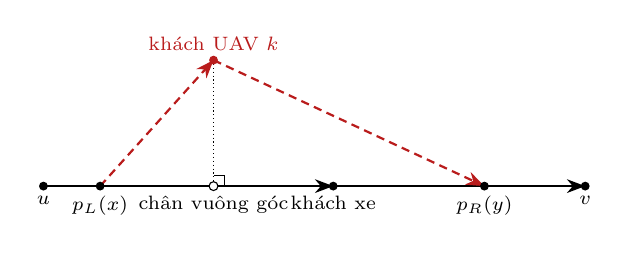
\begin{tikzpicture}[>=Stealth,scale=.80, every node/.style={font=\scriptsize}]
\coordinate (u) at (0,0);\coordinate (a) at (4.6,0);\coordinate (v) at (8.6,0);
\coordinate (k) at (2.7,2.0);\coordinate (f) at (2.7,0);
\coordinate (l) at (0.9,0);\coordinate (r) at (7.0,0);
\draw[thick,->] (u)--(a);\draw[thick,->] (a)--(v);
\draw[densely dotted] (k)--(f);
\draw[thin] (f) ++(0.17,0) -- ++(0,0.17) -- ++(-0.17,0);
\draw[densely dashed,->,thick,hred] (l)--(k);\draw[densely dashed,->,thick,hred] (k)--(r);
\fill (u) circle(2pt) node[below] {$u$};
\fill (a) circle(2pt) node[below] {khách xe};
\fill (v) circle(2pt) node[below] {$v$};
\fill[hred] (k) circle(2pt) node[above] {khách UAV $k$};
\fill (l) circle(2pt) node[below] {$p_L(x)$};
\fill (r) circle(2pt) node[below] {$p_R(y)$};
\filldraw[fill=white] (f) circle(2pt);
\node[below] at (f) {chân vuông góc};
\end{tikzpicture}
\vspace{4pt}
\ghichu{\textbf{Hình 1.} Một lượt bay với điểm gặp trên cạnh. Xe (đường liền) đi từ $u$, qua một khách của xe, tới $v$;
UAV (nét đứt) cất cánh tại $p_L(x)$ trên cạnh đầu, giao cho khách $k$ rồi được thu hồi tại $p_R(y)$ trên cạnh cuối.
Chân đường vuông góc hạ từ $k$ là điểm trên cạnh đầu gần khách nhất. Tại điểm thu hồi đồng bộ, xe và UAV tới cùng lúc (Mục 4.3).}
\end{columns}
\end{frame}

\begin{frame}{Dừng giữa cạnh, chờ, pin và sạc\src{Mục 3.1--3.2}}
\begin{columns}[T,onlytextwidth]
\column{0.49\textwidth}
\begin{block}{Dừng và chờ}
\footnotesize
\begin{itemize}
\item Xe \textbf{dừng hẳn} tại điểm gặp.
\item Dừng giữa cạnh tốn thêm $s^{\rm edge}_L$ (cất cánh) và $s^{\rm edge}_R$ (thu hồi); trong thí nghiệm hai giá trị bằng nhau, ký hiệu chung $s^{\rm edge}$.
\item Dừng \textbf{tại nút} không tốn khoản này; điểm cất cánh trùng điểm thu hồi $\Rightarrow$ chỉ tính \textbf{một lần dừng}.
\item Bên tới điểm thu hồi trước phải \textbf{chờ} bên kia; kịch bản chính: UAV chờ bằng \textbf{bay treo}.
\end{itemize}
\end{block}
\column{0.49\textwidth}
\begin{block}{Pin và sạc}
\footnotesize
\begin{itemize}
\item UAV được sạc \textbf{khi ở trên xe}, tốc độ $r_c$, tối đa tới dung lượng $B$.
\item Trước khi cất cánh, xe có thể \textbf{đứng chờ sạc vừa đủ} cho lượt bay cộng mức dự trữ $b_{\min}$.
\item Một điểm gặp ảnh hưởng \textbf{không chỉ lượt bay chứa nó}: thu hồi muộn hơn $\Rightarrow$ UAV ở trên xe ít hơn $\Rightarrow$ sạc ít hơn $\Rightarrow$ có thể buộc xe chờ sạc trước lượt sau.
\end{itemize}
\end{block}
\end{columns}
\vspace{4pt}
\begin{alertblock}{Hệ quả cho cách đánh giá}
\footnotesize Thời điểm giao và mức pin phải được \textbf{tính lần lượt theo trình tự vận hành}; không thể cộng riêng quãng đường của xe và của UAV.
Trình tự mô phỏng và các trường hợp biên: Phụ lục A.
\end{alertblock}
\end{frame}

\begin{frame}{Phương án và ràng buộc\src{Mục 3.3}}
\begin{itemize}\footnotesize
\item Phương án $z=(r,\mathcal S,\xi)$: tuyến xe $r=(0,r_1,\ldots,r_q,0')$ liệt kê khách do xe phục vụ ($0'$: bản sao kho cuối tuyến).
\item Lượt bay $s=(i_s,k_s,j_s)\in\mathcal S$ gắn với \textbf{đoạn phối hợp} từ nút xe $i_s$ tới nút xe $j_s$, phục vụ khách $k_s$; $\xi_s=(x_s,y_s)$ xác định điểm cất cánh trên cạnh đầu và điểm thu hồi trên cạnh cuối. Mỗi khách được phục vụ \textbf{đúng một lần}, bởi xe hoặc một lượt bay.
\item Đoạn phối hợp bắt đầu khi hai phương tiện \textbf{cùng sẵn sàng} tại $i_s$ và kết thúc khi đã tới $j_s$, thu hồi UAV và làm xong việc tại nút đó (gồm cả thời gian xe chở UAV trước cất cánh và sau thu hồi).
\item Hai đoạn liên tiếp \textbf{có thể chung nút ranh giới nhưng không chung cạnh} $\Rightarrow$ biểu diễn phương án bằng cách \textbf{chia thứ tự khách thành các đoạn} (Mục 4.4), đổi lại loại các phương án có nhiều lần cất cánh--thu hồi trên cùng một cạnh.
\item Vùng dừng: $\mathcal Z_L,\mathcal Z_R\subseteq[0,1]$ là tập phân số được phép dừng trên cạnh cất cánh / thu hồi; không hạn chế thì bằng $[0,1]$; có vùng dừng thì gồm các khoảng đóng được phép cộng hai đầu mút.
\end{itemize}
\vspace{-2pt}
\begin{equation}\tag{1}
\mathcal X_s=\{(x,y)\in\mathcal Z_L\times\mathcal Z_R:\ y\ge x\ \text{nếu hai điểm cùng cạnh}\}
\end{equation}
{\footnotesize Một cặp vị trí thuộc $\mathcal X_s$ \textbf{chưa chắc khả thi về pin}; tính khả thi được kiểm tra khi mô phỏng (Phụ lục A).\par}
\end{frame}

\begin{frame}{Giả thiết vận hành\src{Mục 3.3}}
\begin{columns}[T,onlytextwidth]
\column{0.49\textwidth}
\begin{block}{Xác định và biết trước}
\footnotesize
\begin{itemize}
\item Vận tốc và công suất \textbf{xác định, biết trước}.
\item Không xét gió, ùn tắc ngẫu nhiên hay tranh chấp chỗ dừng.
\item Thời gian thao tác tính riêng, không gộp với chi phí dừng giữa cạnh:
  chuẩn bị cất cánh $s_L$, thu hồi $s_R$, cất cánh $t_{\rm to}$, hạ cánh $t_{\rm ld}$, giao hàng bằng UAV $t_{\rm sv}$.
\end{itemize}
\end{block}
\column{0.49\textwidth}
\begin{block}{Pin và hạn giao}
\footnotesize
\begin{itemize}
\item Pin ban đầu \textbf{đầy}.
\item Lượt bay chỉ được thực hiện nếu \textbf{năng lượng cần dùng + mức dự trữ $\le B$}, sau khi đã tính thời gian chờ sạc.
\item Hạn giao \textbf{mềm}: giao trễ bị phạt trong hàm mục tiêu nhưng không làm phương án bất khả thi.
\item \textbf{Không có giờ mở cửa} buộc xe phải chờ.
\end{itemize}
\end{block}
\end{columns}
\vspace{6pt}
\begin{exampleblock}{Vì sao các giả thiết này quan trọng}
\footnotesize Quy tắc loại nhãn của bộ giải mã (Mục 4.4, Phụ lục F) dựa trên: không có giờ mở cửa, thời gian xác định,
nhiều pin hơn không bất lợi, và chi phí tăng theo thời điểm giao.
\end{exampleblock}
\end{frame}

\begin{frame}{Hàm mục tiêu\src{Mục 3.4}}
\footnotesize
Ba mối quan tâm: \textbf{giao trễ cho khách ưu tiên là tệ nhất}; ngay cả khi đúng hạn, \textbf{giao sớm vẫn tốt hơn}; \textbf{năng lượng UAV cũng có chi phí}.
Với $C_i$ là thời điểm giao xong cho khách $i$, $e_s$ là năng lượng của lượt bay $s$, $W=\sum_{i\in V}w_i$, $\pos{u}=\max\{0,u\}$:
\begin{equation}\tag{2}
J=\underbrace{10\,\frac{\sum_{i\in V}w_i\pos{C_i-d_i}}{W\Dref}}_{10\,T_w}
 +\underbrace{\frac{\sum_{i\in V}w_iC_i}{W\Dref}}_{D_w}
 +\underbrace{0{,}1\,\frac{\sum_{s\in\mathcal S}e_s}{\Eref}}_{0{,}1\,E}
\end{equation}
\begin{columns}[T,onlytextwidth]
\column{0.49\textwidth}
\begin{itemize}
\item $T_w$: trễ hạn có trọng số; $D_w$: thời điểm giao có trọng số; $E$: năng lượng --- đều \textbf{đã chuẩn hóa}.
\item Hệ số \textbf{10} đặt giảm trễ hạn lên hàng đầu; \textbf{0,1} giữ năng lượng ở vai trò phụ; \textbf{như nhau cho mọi phương pháp}.
\item Makespan $M$ (thời điểm xe về kho) và \textbf{tỷ lệ khách giao đúng hạn} được báo riêng, không gộp vào $J$.
\end{itemize}
\column{0.48\textwidth}
\begin{block}{Hai tính chất dùng cho quy tắc loại nhãn}
\footnotesize
\begin{itemize}
\item Không có giờ mở cửa.
\item Nhờ số hạng $D_w$: mỗi đơn vị thời gian giao muộn hơn làm chi phí của khách $i$ tăng \textbf{ít nhất} $w_i/(W\Dref)$.
\end{itemize}
\end{block}
\end{columns}
\end{frame}

\begin{frame}{Mốc chuẩn hóa và độ khó\src{Mục 3.4--3.5}}
\begin{columns}[T,onlytextwidth]
\column{0.53\textwidth}
\begin{block}{Mốc chuẩn hóa (cố định cho từng bài, trước mọi thuật toán)}
\footnotesize
\begin{itemize}
\item Không phương pháp nào thay đổi được thước đo của chính nó.
\item $\Dref$: thời điểm giao trung bình có trọng số trên một \textbf{tuyến tham chiếu chỉ có xe}, dựng bằng Lin--Kernighan--Helsgaun (LKH)~\cite{lkh2000}.
\item $\Eref$: tổng năng lượng các \textbf{chuyến bay khứ hồi giả định} từ nút gần nhất tới từng khách được phép giao bằng UAV.
\item Đơn vị thời gian $\tau$: \textbf{trung vị} thời gian các chặng xe có độ dài dương trên tuyến tham chiếu; mọi thời gian thao tác và chi phí dừng đo bằng \textbf{bội của $\tau$}.
\item Các mốc chỉ dùng làm thang đo; công thức sinh hạn giao và tham số năng lượng ở Phụ lục B.
\end{itemize}
\end{block}
\column{0.44\textwidth}
\begin{alertblock}{Bài toán là NP-khó}
\footnotesize
Gọi $\mathcal F$ là tập phương án thỏa mọi điều kiện; bài toán là $\min_{z\in\mathcal F}J(z)$.
\begin{itemize}
\item Ngay cả khi \textbf{bỏ UAV}: đặt mọi $w_i=1$, thời gian phục vụ bằng 0, hạn giao đủ rộng $\Rightarrow$ số hạng trễ và năng lượng biến mất.
\item $J$ chỉ còn là tổng thời điểm tới khách nhân hằng số dương: mục tiêu của bài toán \textbf{minimum latency}, vốn NP-khó~\cite{blum1994}.
\item GEMS khai thác bài toán con khi \textbf{cố định thứ tự khách} để xây dựng một heuristic (Mục 4.4).
\end{itemize}
\end{alertblock}
\end{columns}
\end{frame}
%% ============================================================== 4. Phương pháp
\section{Phương pháp đề xuất: GEMS}

\begin{frame}{Tổng quan GEMS\src{Mục 4 \textperiodcentered{} Hình 2}}
\begin{itemize}\footnotesize
\item Dành \textbf{phần lớn thời gian để tìm thứ tự khách hàng} (giải mã tại nút), rồi dùng \textbf{hình học} khai thác thêm phương án phối hợp trên thứ tự tốt nhất $\Rightarrow$ khảo sát được nhiều thứ tự mà vẫn xét điểm gặp giữa cạnh ở lời giải cuối.
\item Cả hai tầng dùng \textbf{chung hàm mục tiêu (2)} và \textbf{chung bộ mô phỏng thời gian--pin}.
\end{itemize}
\vspace{4pt}
\centering
\resizebox{\textwidth}{!}{%
\begin{tikzpicture}[>=Stealth,font=\footnotesize,
box/.style={draw=navy,rounded corners=2pt,align=center,inner sep=5pt,minimum height=1.5cm,fill=soft}]
\node[box,text width=3.1cm] (init) at (0,0) {\textbf{Khởi tạo quần thể}\\tìm kiếm cục bộ từ\\nhiều điểm xuất phát};
\node[box,text width=3.5cm] (search) at (4.1,0) {\textbf{Tìm thứ tự tại nút}\\lai ghép $\to$ sàng lọc\\$\to$ tìm kiếm cục bộ};
\node[box,text width=3.5cm,fill=tealc!10,draw=tealc] (geo) at (8.5,0) {\textbf{Giải mã hình học}\\điểm gặp ứng viên\\$+$ DP thời gian--pin};
\node[box,text width=2.6cm,fill=hred!7,draw=hred] (out) at (12.4,0) {\textbf{Phương án}\\phân công khách\\lượt bay, lịch giao};
\draw[->,thick] (init)--(search);
\draw[->,thick] (search)--node[above] {$\pi^*$} (geo);
\draw[->,thick] (geo)--(out);
\draw[<->] (-1.6,-1.2)--node[below] {ngân sách tìm kiếm $T_s=T-R(n)$} (5.9,-1.2);
\draw[<->] (6.7,-1.2)--node[below] {thời gian dự trữ $R(n)$} (10.3,-1.2);
\end{tikzpicture}}
\ghichu{\textbf{Hình 2.} Quy trình GEMS: khởi tạo quần thể bằng multi-start, cải thiện thứ tự bằng tìm kiếm memetic và giải mã hình học để bố trí lại lượt bay. Lời giải tốt nhất đã hoàn tất được giữ xuyên suốt quá trình.}
\vspace{2pt}
\begin{columns}[T,onlytextwidth]
\column{0.32\textwidth}\centering{\footnotesize\color{navy}\textbf{Chọn thứ tự nào?}\\ multi-start + memetic có sàng lọc (4.1--4.2)}
\column{0.32\textwidth}\centering{\footnotesize\color{navy}\textbf{Xét những điểm gặp nào?}\\ đầu mút, chân vuông góc, điểm đồng bộ (4.3)}
\column{0.32\textwidth}\centering{\footnotesize\color{navy}\textbf{Ghép lượt bay ra sao?}\\ QHĐ trên nhãn thời gian--pin (4.4)}
\end{columns}
\end{frame}

\begin{frame}{Khởi tạo quần thể bằng tìm kiếm đa khởi đầu\src{Mục 4.1}}
\begin{columns}[T,onlytextwidth]
\column{0.53\textwidth}
\begin{itemize}\footnotesize
\item Quần thể cần lời giải ban đầu \textbf{đủ tốt và khác nhau} để lai ghép $\Rightarrow$ tạo bằng \textbf{multi-start}.
\item Tập xuất phát: \textbf{tuyến LKH} + \textbf{năm thứ tự tham lam} có xét hạn giao theo chỉ số ATC~\cite{lkh2000,atc1987} (Phụ lục D).
\item \textbf{Bốn thứ tự khác nhau} có điểm giải mã tốt nhất $\to$ chạy LNS \textbf{độc lập} $\Rightarrow$ khai thác nhiều vùng của không gian lời giải trước khi kết hợp trong quần thể.
\item Pha multi-start dùng $0{,}25\,T_s$; mỗi lượt LNS nhận \textbf{tối đa một phần tư} ngân sách pha này.
\item Lời giải đã hoàn tất $\to$ quần thể; bổ sung \textbf{biến thể xáo trộn} để đạt \textbf{12 cá thể} khi còn thời gian.
\item Phần còn lại của $T_s$: tìm kiếm trong quần thể. Lời giải tốt nhất được giữ qua cả hai pha.
\item LNS tạm loại \textbf{3 hoặc 16} khách mỗi vòng (pha multi-start); \textbf{3 hoặc 8} khách (pha quần thể).
\item Tỷ lệ 25\% được chọn trên \textbf{dữ liệu phát triển} và cố định trước đánh giá (Mục 5.1).
\end{itemize}
\column{0.44\textwidth}
\centering
\begin{tikzpicture}[font=\scriptsize,>=Stealth,scale=0.95]
\fill[navy!75] (0,0) rectangle (1.45,0.55);
\fill[navy!40] (1.45,0) rectangle (5.8,0.55);
\fill[tealc!55] (5.8,0) rectangle (6.6,0.55);
\node[white,font=\scriptsize\bfseries] at (0.725,0.275) {multi-start};
\node[white,font=\scriptsize\bfseries] at (3.6,0.275) {tìm kiếm trong quần thể};
\node[font=\scriptsize\bfseries,white] at (6.2,0.275) {$R(n)$};
\draw[decorate,decoration={brace,amplitude=4pt}] (0,0.65)--(1.45,0.65) node[midway,above=4pt] {$0{,}25\,T_s$};
\draw[decorate,decoration={brace,amplitude=4pt}] (1.45,0.65)--(5.8,0.65) node[midway,above=4pt] {$0{,}75\,T_s$};
\draw[decorate,decoration={brace,amplitude=4pt,mirror}] (0,-0.1)--(5.8,-0.1) node[midway,below=4pt] {$T_s=T-R(n)$: tìm thứ tự (giải mã tại nút)};
\draw[decorate,decoration={brace,amplitude=4pt,mirror}] (5.8,-0.85)--(6.6,-0.85) node[midway,below=4pt,align=center] {giải mã\\cuối};
\node[anchor=west] at (0,-1.55) {$T=60$~s; $R(n)=1{,}0/3{,}0/2{,}5$~s ở $n=50/100/175$};
\end{tikzpicture}
\vspace{6pt}
\begin{block}{Bốn lượt LNS độc lập}
\scriptsize
Mỗi lượt từ một trong bốn thứ tự có điểm giải mã tốt nhất trong \{tuyến LKH, 5 thứ tự ATC\}; mỗi lượt $\le\frac14$ ngân sách pha.
\end{block}
\end{columns}
\end{frame}

\begin{frame}{Tìm kiếm memetic và sàng lọc cá thể\src{Mục 4.2}}
\begin{columns}[T,onlytextwidth]
\column{0.52\textwidth}
\begin{itemize}\footnotesize
\item Cá thể lưu \textbf{một hoán vị khách hàng} và phương án xe--UAV do bộ giải mã dựng từ hoán vị đó.
\item \textbf{Lai ghép} tạo thứ tự mới; \textbf{LNS} cải thiện bằng cách tạm loại một nhóm khách rồi chèn lại vào tuyến xe hoặc lượt bay. Giai đoạn này dùng \textbf{giải mã tại nút}.
\item Tìm kiếm cục bộ đắt hơn giải mã sơ bộ: bài 174 khách, một lần LNS $\approx$ \textbf{0,25~s}, giải mã 8 nhãn $\approx$ \textbf{0,9~ms}.
\item $\Rightarrow$ tạo \textbf{nhiều} cá thể con nhưng \textbf{chỉ cải thiện} cá thể có điểm giải mã tốt nhất trong tập $\mathcal C$ gồm $K=16$ cá thể sinh bằng lai ghép thứ tự tuyến tính (LOX):
\end{itemize}
\begin{equation}\tag{3}
\pi^\circ=\arg\min_{\pi\in\mathcal C}\Jhat(\pi)
\end{equation}
\begin{itemize}\footnotesize
\item $\Jhat(\pi)$: $J$ của phương án khả thi dựng bằng bộ giải mã giới hạn \textbf{8 nhãn} --- đánh giá nhanh trực tiếp từ mô hình, \textbf{không cần dữ liệu huấn luyện}.
\end{itemize}
\column{0.45\textwidth}
\centering
\begin{tikzpicture}[font=\scriptsize,>=Stealth,node distance=0.32cm,
st/.style={draw=navy,fill=soft,rounded corners=2pt,align=center,inner sep=3pt,text width=4.6cm}]
\node[st] (p) {chọn hai bố mẹ $p_1,p_2$ (đấu cặp)};
\node[st,below=of p] (c) {$K=16$ cá thể con bằng LOX$(p_1,p_2)$};
\node[st,below=of c,fill=tealc!10,draw=tealc] (s) {giải mã mỗi con với $L{=}8$;\\ chọn $\pi^\circ$ có $\Jhat$ nhỏ nhất};
\node[st,below=of s] (d) {giải mã lại $\pi^\circ$ với $L{=}64$};
\node[st,below=of d] (l) {100 vòng LNS (loại--chèn thích nghi)};
\node[st,below=of l,fill=hred!7,draw=hred] (q) {thêm vào quần thể; sau 20 cá thể mới giữ 12};
\foreach \a/\b in {p/c,c/s,s/d,d/l,l/q} \draw[->,thick] (\a)--(\b);
\end{tikzpicture}
\vspace{2pt}
\ghichu{Quần thể theo chất lượng và độ đa dạng~\cite{vidal2012}, ưu tiên loại bản trùng; phép loại--chèn chọn thích nghi~\cite{ropke2006}. Chi tiết: Phụ lục D; đánh giá: Mục 6.5.}
\end{columns}
\end{frame}

\begin{frame}{Vòng lặp tìm kiếm có sàng lọc\src{Thuật toán 2 \textperiodcentered{} Phụ lục D}}
\begin{columns}[T,onlytextwidth]
\column{0.60\textwidth}
\setcounter{algorithm}{1}
\begin{algorithm}[H]
\caption{Vòng lặp tìm kiếm có sàng lọc trong GEMS}
\scriptsize
\begin{algorithmic}[1]
\Require bài toán; mốc dừng; quần thể $\mathcal P$ và lời giải tốt nhất $z^*$ sau khởi tạo; số cá thể con $K$
\Ensure lời giải tốt nhất $z^{*}$
\While{chưa hết thời gian}
\State chọn hai bố mẹ $p_1,p_2\in\mathcal{P}$
\State $\mathcal{C}\gets K$ cá thể con $\mathrm{LOX}(p_1,p_2)$ \Comment{tạo cá thể con}
\State $\pi^{\circ}\gets\arg\min_{\pi\in\mathcal{C}}\Jhat(\pi)$ \Comment{sàng lọc, $L=8$}
\State $z\gets$ giải mã $\pi^{\circ}$ với $L=64$
\State $z\gets\mathrm{LNS}(z)$ với 100 vòng lặp
\State thêm $z$ vào $\mathcal{P}$; nếu $J(z)<J(z^{*})$ thì $z^{*}\gets z$
\State nếu $|\mathcal{P}|=32$: thu gọn về 12 cá thể
\State nếu 128 cá thể con liên tiếp không cải thiện $z^{*}$: tăng đa dạng của $\mathcal{P}$
\EndWhile
\State \Return $z^{*}$
\end{algorithmic}
\end{algorithm}
\column{0.37\textwidth}
\begin{block}{Ghi chú}
\scriptsize
\begin{itemize}
\item GEMS nhận quần thể từ multi-start (Mục 4.1); đối chứng \emph{khởi tạo trực tiếp} nhận 6 thứ tự kiến tạo + 6 biến thể xáo trộn, mỗi cá thể giải mã $L=64$ rồi LNS.
\item Sau khởi tạo, \textbf{cả hai} dùng cùng vòng lặp này.
\item $|\mathcal P|$: 12 cá thể + 20 con mới $=32$ $\to$ thu gọn về 12.
\item Tăng đa dạng: giữ 4 cá thể tốt nhất + biến thể xáo trộn của $z^*$ và các thứ tự ban đầu.
\end{itemize}
\end{block}
\end{columns}
\end{frame}

\begin{frame}{Sinh điểm gặp hình học: ba loại ứng viên\src{Mục 4.3}}
\begin{columns}[T,onlytextwidth]
\column{0.50\textwidth}
\begin{itemize}\scriptsize
\item Mỗi cặp điểm mới tạo thêm \textbf{một cách phối hợp} phải đánh giá từ \textbf{nhiều trạng thái pin và thời gian} $\Rightarrow$ thay lưới dày bằng ba loại vị trí có vai trò rõ ràng:
\begin{enumerate}
\item \textbf{Đầu mút}: tránh chi phí dừng giữa cạnh.
\item \textbf{Chân đường vuông góc} từ khách UAV xuống cạnh: rút ngắn chặng bay.
\item \textbf{Điểm đồng bộ}: hai phương tiện tới điểm thu hồi \textbf{cùng lúc}.
\end{enumerate}
\item \textbf{Phía thu hồi} (cố định điểm cất cánh, dịch điểm thu hồi dọc cạnh cuối): xe tới trước $\to$ thu hồi muộn hơn giảm thời gian xe chờ; xe đã tới sau $\to$ dịch tiếp không làm hai phương tiện rời cuối cạnh sớm hơn, UAV phải treo chờ và còn ít thời gian sạc.
\item UAV nhanh hơn xe, chi phí dừng không đổi, không chờ sạc, điều kiện công suất treo (Phụ lục E) $\Rightarrow$ \textbf{ranh giới đồng bộ là điểm thu hồi sớm nhất trong miền xe không phải chờ}.
\item \textbf{Phía cất cánh}: đánh đổi ngược --- đi xa hơn trên xe tiết kiệm năng lượng bay treo nhưng khách UAV nhận hàng muộn hơn $\Rightarrow$ giữ lựa chọn \textbf{cả hai phía} để cân đối thời gian giao và pin.
\end{itemize}
\column{0.47\textwidth}
\centering
\begin{tikzpicture}[>=Stealth,scale=0.78,every node/.style={font=\scriptsize}]
\coordinate (u) at (0,0);\coordinate (a) at (4.0,0);\coordinate (v) at (7.6,0);
\coordinate (k) at (2.3,2.3);
\draw[thick,->] (u)--(a);\draw[thick,->] (a)--(v);
\node[below=5pt] at (2.0,-0.35) {cạnh cất cánh};
\node[below=5pt] at (5.8,-0.35) {cạnh thu hồi};
\draw[densely dotted] (k)--(2.3,0);
\draw[thin] (2.3,0) ++(0.15,0) -- ++(0,0.15) -- ++(-0.15,0);
\draw[densely dashed,->,hred,thick] (1.1,0)--(k);
\draw[densely dashed,->,hred,thick] (k)--(5.7,0);
\fill[hred] (k) circle(2.2pt) node[above] {khách UAV $k$};
\foreach \p in {u,a,v} \fill[navy] ($(\p)+(-0.11,-0.11)$) rectangle ($(\p)+(0.11,0.11)$);
\filldraw[fill=white,draw=navy,thick] (2.3,0) circle(2.6pt);
\node[diamond,fill=tealc,inner sep=1.6pt] at (1.1,0) {};
\node[diamond,fill=tealc,inner sep=1.6pt] at (5.7,0) {};
\node[above=2pt] at (u) {$u$};\node[below=2pt] at (v) {$v$};
\node[above right=1pt] at (5.7,0) {đồng bộ};
\node[above left=1pt] at (1.1,0.05) {đồng bộ};
\end{tikzpicture}
\vspace{4pt}

\scriptsize
\begin{tabular}{@{}cl@{}}
\tikz\fill[navy] (0,0) rectangle (0.2,0.2); & đầu mút (luôn có, không tốn dừng)\\
\tikz\filldraw[fill=white,draw=navy,thick] (0,0) circle(2.6pt); & chân đường vuông góc\\
\tikz\node[diamond,fill=tealc,inner sep=1.6pt] {}; & điểm đồng bộ (cất cánh hoặc thu hồi)\\
\end{tabular}
\ghichu{Minh họa vị trí tương đối; tọa độ không theo tỷ lệ.}
\end{columns}
\end{frame}

\begin{frame}{Điểm đồng bộ: cách tính và phạm vi\src{Mục 4.3}}
\footnotesize
Gọi $T_T(x,y)$ và $T_U(x,y)$ là thời gian \textbf{xe sẵn sàng} và \textbf{UAV tới} điểm thu hồi, cùng đo từ sau chuẩn bị cất cánh. Điểm đồng bộ thỏa
\begin{equation}\tag{4}
T_T(x,y)=T_U(x,y).
\end{equation}
\begin{columns}[T,onlytextwidth]
\column{0.50\textwidth}
\begin{block}{Bộ sinh ứng viên}
\scriptsize
\begin{enumerate}
\item Cố định điểm cất cánh tại \textbf{đầu cạnh} hoặc \textbf{chân đường vuông góc} $\to$ tìm \textbf{điểm thu hồi đồng bộ}.
\item Cố định điểm thu hồi tại \textbf{cuối cạnh} hoặc \textbf{chân đường vuông góc} $\to$ tìm \textbf{điểm cất cánh đồng bộ}.
\item Đoạn thẳng: giải trực tiếp sau khi đưa về \textbf{bậc hai}; đường gấp khúc: xét lần lượt từng đoạn.
\item \textbf{Luôn thêm các cặp đầu mút}.
\item Mọi nghiệm phải thỏa vùng dừng, thứ tự xe di chuyển và \textbf{phương trình gốc} (Phụ lục E).
\end{enumerate}
\end{block}
\column{0.47\textwidth}
\begin{block}{Dùng chung và tính lại}
\scriptsize
\begin{itemize}
\item Tập điểm được tạo \textbf{một lần cho mỗi đoạn} rồi dùng chung cho các nhãn.
\item Chi phí và tính khả thi \textbf{vẫn được tính lại} theo thời gian và pin đầu vào của từng nhãn.
\end{itemize}
\end{block}
\begin{alertblock}{Không phải liệt kê điểm tối ưu liên tục}
\scriptsize Đây là một cách chọn ứng viên \textbf{có cơ sở hình học}. Giá trị của tập điểm được đánh giá bằng cả chất lượng toàn tuyến lẫn thời gian giải mã (Mục 6.4).
\end{alertblock}
\end{columns}
\end{frame}

\begin{frame}{Giải mã bằng quy hoạch động thời gian--pin\src{Mục 4.4}}
\begin{columns}[T,onlytextwidth]
\column{0.51\textwidth}
\begin{itemize}\scriptsize
\item Điểm gặp tốt chỉ hữu ích nếu được ghép vào lịch trình phù hợp $\Rightarrow$ giải mã lại \textbf{toàn bộ} thứ tự $\pi=(0,\pi_1,\ldots,\pi_m,0')$, cho phép \textbf{đổi khách do UAV phục vụ} và các đoạn lượt bay.
\item Đoạn từ vị trí $i$ tới $j$: xe phục vụ mọi khách, \textbf{hoặc} UAV phục vụ một khách $\pi_k$ ($i<k<j$), xe giữ thứ tự các khách còn lại; các đoạn nối tiếp tạo thành phương án đầy đủ.
\item Chỉ giữ phương án chi phí thấp nhất tại mỗi vị trí \textbf{chưa đủ}: phương án đó có thể tới muộn hoặc còn ít pin, bất lợi cho phần sau $\Rightarrow$ giữ nhiều \textbf{nhãn} $(g,t,b)$: chi phí đã tích lũy, thời điểm hai phương tiện sẵn sàng, pin còn lại.
\item Chuyển tiếp $a:i\to j$ chọn đoạn xe, khách UAV và cặp điểm gặp; bộ mô phỏng trả về thời điểm kết thúc $\Phi_a(t,b)$, pin còn lại $\Psi_a(b)$, năng lượng $e_a$ và thời điểm giao $C_v^a(t,b)$ của từng khách vừa phục vụ.
\item Bắt đầu từ $(0,0,B)$ tại kho; chọn nhãn có $g$ nhỏ nhất ở kho cuối. Mỗi khách chỉ tính một lần; mang theo $(t,b)$ $\Rightarrow$ đánh giá tác động của một điểm gặp lên \textbf{các lượt bay phía sau}.
\end{itemize}
\column{0.46\textwidth}
\centering
\begin{tikzpicture}[font=\scriptsize,>=Stealth,x=0.6cm]
\foreach \i/\lab in {0/0,1/\pi_1,2/\cdots,3/\pi_i,4/\pi_{i+1},5/\pi_k,6/\pi_{j-1},7/\pi_j,8/\cdots,9/0'}
  {\fill[navy] (\i,0) circle(1.6pt); \node[below=2pt] at (\i,0) {$\lab$};}
\draw[thick,navy] (0,0)--(9,0);
\draw[->,thick,hred,densely dashed] (3,0.08) .. controls (4,1.2) and (4.6,1.3) .. (5,1.08);
\draw[->,thick,hred,densely dashed] (5,1.08) .. controls (5.6,1.3) and (6.4,1.2) .. (7,0.08);
\fill[hred] (5,1.08) circle(1.8pt) node[above] {UAV: $\pi_k$};
\draw[decorate,decoration={brace,amplitude=4pt,mirror}] (3,-0.55)--(7,-0.55) node[midway,below=4pt] {chuyển tiếp $a:i\to j$; nhãn mới tại $j$};
\end{tikzpicture}
\vspace{2pt}
\begin{block}{Chi phí một khách và nhãn mới}
\scriptsize
Chi phí của khách $v$ khi giao tại thời điểm $C$:
\begin{equation}\tag{5}
\varphi_v(C)=\frac{w_v}{W\Dref}\bigl(10\pos{C-d_v}+C\bigr)
\end{equation}
Với $U_a=\{\pi_{i+1},\ldots,\pi_j\}\cap V$ (khách phục vụ trong đoạn):
\begin{equation}\tag{6}
\begin{aligned}
g'&=g+\textstyle\sum_{v\in U_a}\varphi_v\bigl(C_v^a(t,b)\bigr)+0{,}1\,e_a/\Eref,\\
t'&=\Phi_a(t,b),\qquad b'=\Psi_a(b).
\end{aligned}
\end{equation}
\end{block}
\end{columns}
\end{frame}

\begin{frame}{Quy tắc trội và trần nhãn\src{Mục 4.4}}
\begin{columns}[T,onlytextwidth]
\column{0.52\textwidth}
\begin{itemize}\footnotesize
\item Khai thác \textbf{lợi thế của việc tới sớm}: $W_j^+$ = tổng trọng số khách chưa phục vụ sau vị trí $j$; $\kappa_j=W_j^+/(W\Dref)$.
\item Tới sớm hơn $\Delta t$ mà \textbf{không có ít pin hơn} $\Rightarrow$ cùng một cách đi tiếp giảm riêng thành phần thời điểm giao ít nhất $\kappa_j\Delta t$.
\item Đặt chi phí hiệu chỉnh $\widehat g=g+\kappa_j t$; \textbf{loại nhãn 2} nếu tồn tại nhãn 1 thỏa
\end{itemize}
\vspace{-4pt}
\begin{equation}\tag{7}
\widehat g_1\le\widehat g_2,\qquad t_1\le t_2,\qquad b_1\ge b_2.
\end{equation}
\vspace{-6pt}
\begin{itemize}\footnotesize
\item So với chỉ so $g$: loại được \textbf{nhiều nhãn hơn} --- nhãn có chi phí quá khứ hơi cao vẫn có thể trội nhờ phục vụ phần còn lại sớm hơn (Phụ lục F).
\end{itemize}
\column{0.45\textwidth}
\begin{block}{Bảo toàn tối ưu khi}
\scriptsize Trên \textbf{tập chuyển tiếp đã liệt kê}, với giả thiết của mô hình:
\begin{itemize}
\item không có giờ mở cửa; thời gian di chuyển xác định;
\item nhiều pin hơn không bất lợi;
\item tập điểm dùng chung cho mọi nhãn.
\end{itemize}
Chứng minh: Phụ lục F.
\end{block}
\begin{alertblock}{Khống chế chi phí (xấp xỉ)}
\scriptsize
\begin{itemize}
\item Giới hạn độ dài đoạn $j-i\le h$.
\item Giữ tối đa $L$ nhãn theo $\widehat g$ --- phần cắt theo $L$ là \textbf{xấp xỉ}; khác biệt với quy tắc trội và sai số quan sát: Phụ lục J.
\end{itemize}
\end{alertblock}
\end{columns}
\end{frame}

\begin{frame}{Phân bổ thời gian: Thuật toán 1\src{Mục 4.5}}
\begin{columns}[T,onlytextwidth]
\column{0.40\textwidth}
\begin{itemize}\footnotesize
\item Dành trước $R(n)$ cho \textbf{giải mã cuối}; tìm kiếm dùng $T_s=T-R(n)$.
\item Sau khi tìm kiếm dừng: giải mã $\pi^*$ \textbf{chỉ bằng đầu mút} rồi mới \textbf{thêm các điểm hình học}.
\item Mỗi lần chỉ thay lời giải đang giữ khi lời giải mới \textbf{đã hoàn tất} và có $J$ \textbf{thấp hơn}.
\item $\Rightarrow$ nếu giải mã hình học không kịp kết thúc, thuật toán \textbf{vẫn trả về phương án khả thi tốt nhất} đã có.
\end{itemize}
\column{0.57\textwidth}
\setcounter{algorithm}{0}
\begin{algorithm}[H]
\caption{GEMS: tìm kiếm memetic kết hợp giải mã hình học}
\footnotesize
\begin{algorithmic}[1]
\Require dữ liệu, thời gian $T$, dự trữ $R(n)$
\State $T_s\gets T-R(n)$; bắt đầu đồng hồ chung
\State chọn bốn thứ tự ban đầu và chạy multi-start trong $0{,}25T_s$
\State khởi tạo quần thể từ các lời giải hoàn tất và các biến thể xáo trộn
\State lai ghép, sàng lọc và cải thiện quần thể đến mốc $T_s$
\State lưu thứ tự tốt nhất $\pi^*$ và phương án tại nút $z$
\For{tập điểm: đầu mút, rồi đầu mút cùng điểm hình học}
\State giải mã $\pi^*$ trong thời gian còn lại
\State thay $z$ nếu lời giải hoàn tất và có $J$ nhỏ hơn
\EndFor
\State \Return $z$
\end{algorithmic}
\end{algorithm}
\end{columns}
\end{frame}

\begin{frame}{Độ phức tạp của một lần giải mã\src{Mục 4.5 \textperiodcentered{} Phụ lục G}}
\begin{columns}[T,onlytextwidth]
\column{0.52\textwidth}
\begin{itemize}\footnotesize
\item Với $Q$ cặp điểm mỗi đoạn có UAV, cài đặt hiện tại cần
\[
\text{thời gian } O\bigl(nh^2[Q^2+QL(h+L)]\bigr),\qquad \text{bộ nhớ } O(nL+n^2).
\]
\item \textbf{Tập điểm nhỏ} giảm số chuyển tiếp; \textbf{trần nhãn} giới hạn số trạng thái phải xét.
\item Thực nghiệm dùng $h=12$ cho mọi lần giải mã.
\end{itemize}
\column{0.45\textwidth}
\footnotesize
\renewcommand{\arraystretch}{1.15}
\begin{tabular}{@{}lcc@{}}
\toprule
\textbf{Lần giải mã} & $L$ & $h$\\\midrule
Sàng lọc cá thể con ($\Jhat$) & 8 & 12\\
Trước tìm kiếm cục bộ & 64 & 12\\
Giải mã lại trong LNS & 8 & 12\\
Giải mã cuối (đầu mút, hình học) & 1024 & 12\\
\bottomrule
\end{tabular}
\ghichu{Giá trị theo Mục 4.5 và bảng tham số (Phụ lục O).}
\end{columns}
\end{frame}
%% ============================================================== 5. Thiết kế thực nghiệm
\section{Thiết kế thực nghiệm}

\begin{frame}{Ba nhóm đánh giá\src{Mục 5 \textperiodcentered{} Bảng 1}}
\footnotesize
Thực nghiệm đánh giá \textbf{phương pháp hoàn chỉnh} trước, sau đó \textbf{tách vai trò} của giải mã hình học và lựa chọn cá thể.
Mức cải thiện giữa các nhóm được \textbf{báo riêng}.
\vspace{4pt}

\renewcommand{\arraystretch}{1.3}
\begin{tabularx}{\textwidth}{@{}P{2.7cm}P{6.1cm}Y@{}}
\toprule
\textbf{Nhóm đánh giá} & \textbf{Thiết kế} & \textbf{Câu hỏi chính}\\\midrule
So sánh phương pháp & 48 bộ tọa độ mới; ba cỡ $n=50,100,175$, bốn họ; mỗi bộ một tốc độ $\alpha=1$ hoặc 3; 60~s & Chất lượng so với HGA-J, ICP-J, multi-start và đối chứng khởi tạo trực tiếp\\\addlinespace
Giải mã hình học & AG: 90 bộ Agatz, hai tốc độ $\alpha=1,3$; MC: 24 bộ nhiều cụm, $\alpha=2$; ba seed, 60~s & Lợi ích của điểm gặp trên cạnh, cơ chế bố trí lại lượt bay và chi phí giải mã\\\addlinespace
Lựa chọn cá thể & 12 bộ Agatz $n=175$, $\alpha=2$; hai seed, 15 và 60~s; chỉ gặp tại nút & Giá trị của tiêu chí sàng lọc trước tìm kiếm cục bộ\\
\bottomrule
\end{tabularx}
\ghichu{\textbf{Bảng 1.} Dữ liệu và vai trò của các phép đánh giá. $n$ gồm kho; $\alpha=v_D/v_T$. Thời hạn, ưu tiên và pin được tạo theo các kịch bản chuẩn hóa. Danh sách đầy đủ các tập con: Phụ lục B.}
\end{frame}

\begin{frame}{Dữ liệu và lựa chọn tham số\src{Mục 5.1}}
\begin{columns}[T,onlytextwidth]
\column{0.50\textwidth}
\begin{block}{Tập xác nhận (48 bộ tọa độ chưa dùng khi phát triển)}
\scriptsize
\begin{itemize}
\item 3 cỡ $\times$ 4 họ phân bố (đồng đều, một cụm, hai cụm, nhiều cụm) $\times$ 4 bộ; trong mỗi tổ hợp \textbf{hai bộ $\alpha=1$, hai bộ $\alpha=3$}.
\item Ba họ đầu: đường xe Euclid; họ nhiều cụm: \textbf{đường chữ L} và vùng dừng cho phép chiếm \textbf{một nửa mỗi cạnh}.
\item Mỗi bộ đi kèm hạn giao, trọng số, điều kiện UAV: khách khẩn \textbf{30--40\%}, trọng số \textbf{5} (còn lại 1); khoảng \textbf{80\%} khách được giao bằng UAV.
\end{itemize}
\end{block}
\begin{block}{AG và MC (phân tích bộ giải mã)}
\scriptsize
\begin{itemize}
\item \textbf{AG}: 90 bộ tọa độ Agatz~\cite{agatz2018}, hạn giao theo khoảng cách từ kho. \textbf{MC}: 24 bộ nhiều cụm, hạn giao theo thời điểm tới trên tuyến tham chiếu, pin và vùng dừng khác AG.
\item Thứ tự đầu vào do \textbf{đối chứng khởi tạo trực tiếp} tạo ra (Mục 5.2); \textbf{cùng một thứ tự} cho cả hai cách giải mã; MC được sinh \textbf{sau} khi cố định đối chứng này.
\end{itemize}
\end{block}
\column{0.47\textwidth}
\begin{alertblock}{Tách dữ liệu phát triển và đánh giá}
\scriptsize
\begin{itemize}
\item AG và MC đã được dùng trong \textbf{phát triển bộ giải}; 48 bộ xác nhận \textbf{dành riêng} để đánh giá GEMS sau khi cố định phương pháp.
\item Cấu hình tìm kiếm chọn trên \textbf{12 cấu hình phát triển} và một \textbf{tập chọn cấu hình} gồm 12 bộ tọa độ mới (mỗi bộ một seed). Quy tắc: $J$ trung bình thấp hơn.
\item GEMS được chọn \textbf{trước khi chạy tập xác nhận}; trong hai đối chứng HGA-J và ICP-J, \textbf{ICP-J} được chọn làm đối chứng chuyển đổi chính; cả hai vẫn được báo đầy đủ.
\item Tham số, mã và các phép so sánh chính được \textbf{cố định trước đánh giá} (Phụ lục N).
\end{itemize}
\end{alertblock}
\ghichu{Công thức sinh dữ liệu và các tập con: Phụ lục B.}
\end{columns}
\end{frame}

\begin{frame}{Đối chứng: hai bản chuyển đổi và hai cách tổ chức tìm kiếm\src{Mục 5.2}}
\scriptsize
\renewcommand{\arraystretch}{1.25}
\begin{tabularx}{\textwidth}{@{}P{2.6cm}YP{3.3cm}@{}}
\toprule
\textbf{Phương pháp} & \textbf{Cách làm} & \textbf{Kiểm tra điều gì}\\\midrule
\textbf{HGA-J} & Giữ nhiễm sắc thể có loại phương tiện và các toán tử của HGA-TAC~\cite{hgatac2024}; hàm đánh giá thay bằng \textbf{giải mã thời gian--pin trên $J$}. & bản chuyển đổi từ TSP-D\\
\textbf{ICP-J} & Tìm kiếm trên các đoạn liên tiếp theo ICP~\cite{lee2025}; tính mỗi đoạn \textbf{từ thời gian và pin đầu vào} rồi cập nhật phần lịch phía sau. & bản chuyển đổi từ TSP-D (đối chứng chính)\\
\textbf{Multi-start} & Dành \textbf{toàn bộ ngân sách} tìm kiếm cho bốn lượt LNS độc lập. & giá trị của quần thể\\
\textbf{Khởi tạo trực tiếp} & Bỏ pha multi-start của GEMS: quần thể từ tuyến LKH, năm thứ tự ATC và biến thể xáo trộn, mỗi cá thể qua LNS thông thường; dùng toàn bộ ngân sách cho khởi tạo và tiến hóa quần thể. & giá trị của pha multi-start\\
\bottomrule
\end{tabularx}
\vspace{4pt}
\begin{itemize}\scriptsize
\item Hậu tố \textbf{-J}: bản chuyển đổi cho mô hình trong bài; chi tiết cài đặt và đối chiếu mã gốc ở Phụ lục N.
\item Cả năm phương pháp \textbf{tìm thứ tự tại nút} và \textbf{dùng chung bước giải mã cuối} $\Rightarrow$ cùng mô hình đánh giá và cùng khả năng chọn điểm gặp.
\item Bốn phương pháp có ngẫu nhiên chạy \textbf{ba seed}; ICP-J chạy một lượt mỗi bộ $\Rightarrow$ tổng \textbf{624 lượt}. ICP-J xác định khi chạy tới hội tụ, nhưng \textbf{34/48 lượt bị dừng bởi giới hạn thời gian}; biến thiên do thời điểm dừng chưa được đo bằng lặp độc lập.
\item Mọi phương pháp nhận \textbf{cùng dữ liệu đầu vào} và \textbf{cùng ngân sách 60~s}.
\end{itemize}
\end{frame}

\begin{frame}{Phân tích thành phần\src{Mục 5.2}}
\begin{columns}[T,onlytextwidth]
\column{0.49\textwidth}
\begin{block}{Giải mã hình học}
\scriptsize
\begin{itemize}
\item Đối chứng \textbf{chỉ tại nút}: nhận cùng thứ tự $\pi^*$, cùng $h=12$, $L=1024$, nhưng chỉ cho cất cánh và thu hồi tại \textbf{các đầu mút hợp lệ}.
\item Phép so sánh bổ sung: \textbf{giữ nguyên lượt bay} (chỉ thay điểm gặp); \textbf{thay tập điểm bằng lưới}; \textbf{đổi chi phí dừng}.
\end{itemize}
\end{block}
\begin{block}{Kiểm tra lại trên tập con xác nhận}
\scriptsize Một tập con cố định 12 bộ tọa độ xác nhận dùng để kiểm tra lại sàng lọc và \textbf{hai kịch bản vận hành}:
\begin{itemize}
\item dừng $0{,}5\tau$ mỗi phía;
\item giảm dung lượng và dự trữ pin một nửa.
\end{itemize}
\end{block}
\column{0.48\textwidth}
\begin{block}{Sàng lọc cá thể: ba cách chọn}
\scriptsize
\begin{enumerate}
\item tạo \textbf{một} cá thể rồi chạy LNS;
\item tạo \textbf{16} cá thể rồi chọn \textbf{ngẫu nhiên};
\item tạo \textbf{16} cá thể rồi chọn theo \textbf{điểm giải mã}.
\end{enumerate}
Đột biến nhỏ và multi-start là các đối chứng bổ sung.
\end{block}
\begin{exampleblock}{Câu hỏi mà mỗi phép trả lời}
\scriptsize
\begin{itemize}
\item Hình học so với đầu mút: lợi ích của điểm trong cạnh.
\item Giữ nguyên lượt bay: lợi ích đến từ \emph{vị trí} hay từ \emph{bố trí lại}.
\item Chọn ngẫu nhiên cùng 16 ứng viên: tách lợi ích của \emph{tiêu chí chọn} khỏi việc tạo thêm ứng viên.
\end{itemize}
\end{exampleblock}
\end{columns}
\end{frame}

\begin{frame}{Ngân sách tính toán và thống kê\src{Mục 5.3}}
\begin{columns}[T,onlytextwidth]
\column{0.49\textwidth}
\begin{block}{Ngân sách và môi trường}
\scriptsize
\begin{itemize}
\item Thời gian chạy gồm \textbf{khởi tạo, tìm kiếm và giải mã cuối}; tuyến tham chiếu và dữ liệu đầu vào tính trước, dùng chung.
\item $R(n)=1{,}0$; $3{,}0$; $2{,}5$~s ở $n=50,100,175$, cố định từ \textbf{21 bài phát triển}.
\item Lõi C++, điều phối Python; HGA-J dùng mã toán tử Julia. Mỗi lượt \textbf{một luồng}; môi trường làm nóng trước khi đo.
\item AG, khảo sát sàng lọc và tập xác nhận: Xeon 2,8~GHz; MC: Xeon 2,1~GHz $\Rightarrow$ thời gian chỉ đối chiếu \textbf{trong cùng bộ}.
\item Mọi phương án cuối được chấm lại bằng \textbf{bộ đánh giá Python độc lập}.
\end{itemize}
\end{block}
\column{0.48\textwidth}
\begin{block}{Mức giảm mục tiêu}
\scriptsize
\begin{equation}\tag{8}
\delta=100\left(1-\frac{J_A}{J_B}\right)\ (\%),\qquad \delta>0\Leftrightarrow A\ \text{tốt hơn}.
\end{equation}
\vspace{-6pt}
\begin{itemize}
\item \textbf{Trung bình các tỷ số ghép cặp} theo bộ tọa độ, không phải tỷ số của hai trung bình $J$.
\item Tập xác nhận, khảo sát sàng lọc: lấy trung bình $J$ qua seed \textbf{trước} khi tính tỷ số. AG/MC: tỷ số từng seed rồi lấy trung bình; hai tốc độ của cùng bộ AG \textbf{gộp trước} suy luận.
\end{itemize}
\end{block}
\begin{block}{Suy luận}
\scriptsize
\begin{itemize}
\item KTC 95\%: bootstrap \textbf{10.000} lần cấp bộ tọa độ~\cite{efron1979} (khảo sát sàng lọc: 5.000).
\item Kiểm định hoán vị dấu hai phía + hiệu chỉnh Holm~\cite{holm1979} cho \textbf{hai nhóm phép chính}: (i) hình học so với đầu mút trên AG và MC; (ii) GEMS so với khởi tạo trực tiếp và ICP-J trên tập xác nhận.
\item Multi-start và các phân tích thành phần: \textbf{thứ cấp}; lát cắt theo cỡ, họ, tốc độ: \textbf{mô tả}. Giao thức đầy đủ: Phụ lục C, P, N.
\end{itemize}
\end{block}
\end{columns}
\end{frame}
%% ============================================================== 6. Kết quả và thảo luận
\section{Kết quả và thảo luận}

\begin{frame}{So sánh với các phương pháp đối chứng\src{Mục 6.1 \textperiodcentered{} Bảng 2}}
\small
\begin{center}
\renewcommand{\arraystretch}{1.18}
\setlength{\tabcolsep}{11pt}
\begin{tabular}{@{}lrrrrr@{}}
\toprule
\textbf{Phương pháp} & $\bar J$ & $\delta$ (\%) & KTC 95\% & Thắng/hòa/thua & $p_{\rm Holm}$\\
\midrule
\rowcolor{hred!7}\textbf{GEMS} & \textbf{1,6790} & \multicolumn{4}{c}{Phương pháp đề xuất}\\
Multi-start & 1,6865 & 0,60 & $[0{,}11;1{,}09]$ & 31/2/15 & --\\
Khởi tạo trực tiếp & 1,6989 & 1,08 & $[0{,}46;1{,}79]$ & 25/12/11 & 0,0012\\
ICP-J & 2,2534 & 24,04 & $[21{,}35;26{,}70]$ & 48/0/0 & $\le 2\cdot10^{-6}$\\
HGA-J & 2,2941 & 25,88 & $[22{,}47;29{,}16]$ & 48/0/0 & --\\
\bottomrule
\end{tabular}
\end{center}
\ghichu{\textbf{Bảng 2.} 48 bộ tọa độ mới, cùng ngân sách 60~s và cùng bộ giải mã cuối. $\bar J$ càng nhỏ càng tốt. Các cột từ $\delta$ trở đi so sánh GEMS với phương pháp ở mỗi dòng; $\delta>0$: GEMS tốt hơn; thắng/hòa/thua đếm từ phía GEMS. KTC 95\% theo bộ tọa độ. ``--'': phép so sánh thứ cấp, không thuộc nhóm kiểm định Holm.}
\vspace{2pt}
\begin{itemize}\footnotesize
\item GEMS đạt $\bar J$ \textbf{thấp nhất} trong năm phương pháp. So với ICP-J và HGA-J: giảm \textbf{24,04\%} và \textbf{25,88\%}, cải thiện ở \textbf{cả 48 bộ}. Các khoảng cách này đánh giá hai \textbf{bản chuyển đổi} trên mô hình khẩn cấp và bộ giải mã chung; đối chiếu mã gốc trên makespan báo riêng (Phụ lục N).
\item Dùng kết quả multi-start để khởi tạo rồi cải thiện bằng quần thể tốt hơn \textbf{cả hai} cách tổ chức riêng lẻ trên mẫu đã xét: 0,60\% so với multi-start dùng toàn bộ ngân sách, 1,08\% so với khởi tạo quần thể trực tiếp ($p_{\rm Holm}=0{,}0012$).
\end{itemize}
\end{frame}

\begin{frame}{Diễn giải theo thời gian giao hàng và theo cỡ bài\src{Mục 6.1}}
\begin{columns}[T,onlytextwidth]
\column{0.53\textwidth}
\centering
{\footnotesize\textbf{Mức giảm của GEMS theo thành phần (\%)}}\\[2pt]
\begin{tikzpicture}
\begin{axis}[width=\linewidth,height=4.6cm,ybar,bar width=11pt,
  ymin=0,ymax=46,xmin=0.45,xmax=2.55,
  xtick={1,2},xticklabels={so với ICP-J,so với HGA-J},
  ytick={0,10,20,30,40},
  tick label style={font=\scriptsize},label style={font=\scriptsize},
  ymajorgrids=true,grid style={black!12},axis x line*=bottom,axis y line*=left,
  nodes near coords,nodes near coords style={font=\tiny},
  /pgf/number format/use comma,/pgf/number format/precision=2,/pgf/number format/fixed,
  legend style={font=\scriptsize,draw=none,at={(0.5,1.02)},anchor=south,legend columns=3,/tikz/every even column/.append style={column sep=6pt}},
  area legend]
\addplot[fill=hred!80,draw=hred] coordinates {(1,32.07) (2,38.04)};
\addlegendentry{trễ hạn $T_w$}
\addplot[fill=navy!70,draw=navy] coordinates {(1,12.97) (2,9.47)};
\addlegendentry{thời điểm giao $D_w$}
\addplot[fill=black!25,draw=black!60] coordinates {(1,24.04) (2,25.88)};
\addlegendentry{$J$ (Bảng 2)}
\end{axis}
\end{tikzpicture}
\ghichu{Tỷ lệ tính sau khi lấy trung bình qua seed trong từng bộ tọa độ, rồi trung bình chênh lệch tương đối trên 48 bộ.}
\column{0.44\textwidth}
\begin{itemize}\scriptsize
\item Phân tích riêng $T_w$ và $D_w$ của các lời giải đã lưu: GEMS giảm \textbf{trễ hạn có trọng số 32,07\%} và \textbf{thời điểm giao có trọng số 12,97\%} so với ICP-J; \textbf{38,04\%} và \textbf{9,47\%} so với HGA-J.
\item Đây là \textbf{phân tích mô tả bổ sung} của cùng các lượt chạy; mức trễ đo \textbf{lượng thời gian giao muộn}, không phải tỷ lệ khách giao trễ; hai chỉ số đều dùng trọng số ưu tiên theo (2).
\end{itemize}
\vspace{2pt}
\centering
{\scriptsize\textbf{So với khởi tạo trực tiếp, theo cỡ bài (\%)}}\\[1pt]
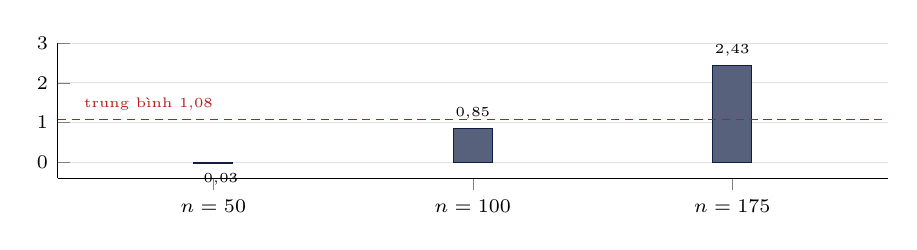
\begin{tikzpicture}
\begin{axis}[width=\linewidth,height=3.3cm,ybar,bar width=14pt,
  ymin=-0.4,ymax=3.0,xmin=0.4,xmax=3.6,
  xtick={1,2,3},xticklabels={$n=50$,$n=100$,$n=175$},
  ytick={0,1,2,3},tick label style={font=\scriptsize},
  ymajorgrids=true,grid style={black!12},axis x line*=bottom,axis y line*=left,
  nodes near coords,nodes near coords style={font=\tiny},
  /pgf/number format/use comma,/pgf/number format/precision=2,/pgf/number format/fixed]
\addplot[fill=navy!70,draw=navy] coordinates {(1,-0.03) (2,0.85) (3,2.43)};
\draw[densely dashed,hred] (axis cs:0.4,1.08)--(axis cs:3.6,1.08) node[pos=0.02,above right,font=\tiny,hred] {trung bình 1,08};
\end{axis}
\end{tikzpicture}
\ghichu{Trung vị trên toàn tập 0,02\% $\Rightarrow$ cải thiện \textbf{không phân bố đều}; lợi ích tập trung ở bài lớn (Phụ lục N).}
\end{columns}
\end{frame}

\begin{frame}{Đóng góp của bộ giải mã hình học\src{Mục 6.2 \textperiodcentered{} Phụ lục C}}
\begin{itemize}\footnotesize
\item Trên các thứ tự do \textbf{đối chứng khởi tạo trực tiếp} tạo ra, giải mã hình học giảm $J$ \textbf{0,74\%} ở AG (KTC [0,63; 0,84]) và \textbf{1,34\%} ở MC ([0,86; 1,99]), cùng ngân sách 60~s; cả hai có $p_{\rm Holm}\le10^{-6}$ --- phần lợi \textbf{bổ sung} sau tìm kiếm tại nút.
\item Ngay cả khi đối chứng dùng \textbf{trọn 60~s} để tìm kiếm tại nút, cách tìm kiếm + giải mã hình học vẫn giảm $J$ \textbf{0,71\%} (AG) và \textbf{1,32\%} (MC).
\item UAV được dùng nhiều hơn để giao sớm hơn: lượt bay \textbf{10,7 $\to$ 11,6} (AG), \textbf{10,4 $\to$ 11,8} (MC); trễ hạn và thời điểm giao cùng giảm, bù cho năng lượng tăng; tỷ lệ khách khẩn đúng hạn gần như giữ nguyên.
\end{itemize}
\vspace{2pt}
\scriptsize
\setlength{\tabcolsep}{3.6pt}
\begin{tabular*}{\textwidth}{@{\extracolsep{\fill}}llrrrrrcc@{}}
\toprule
\textbf{Tập dữ liệu} & \textbf{Cách giải mã} & $10T_w$ & $D_w$ & $0{,}1E$ & $J$ & Lượt UAV & $\delta$ (\%) [KTC 95\%] & T/H/T\\
\midrule
AG (90 bộ) & Chỉ tại nút & 0,70397 & 0,64950 & 0,03629 & 1,38976 & 10,72 & & \\
 & \textbf{Giải mã hình học} & 0,69652 & 0,64788 & 0,03667 & 1,38107 & 11,58 & \textbf{0,74} [0,63; 0,84] & 88/2/0\\
\addlinespace
MC (24 bộ) & Chỉ tại nút & 1,55329 & 0,67064 & 0,02914 & 2,25308 & 10,39 & & \\
 & \textbf{Giải mã hình học} & 1,52509 & 0,66677 & 0,03067 & 2,22253 & 11,78 & \textbf{1,34} [0,86; 1,99] & 23/1/0\\
\bottomrule
\end{tabular*}
\ghichu{Cùng thứ tự, giới hạn 60~s, chi phí dừng $0{,}1\tau$ mỗi phía. Ba cột đầu là ba số hạng của $J$, trung bình trên cấu hình và seed (tổng bằng $J$, sai khác do làm tròn); thắng/hòa/thua (T/H/T) đếm theo bộ tọa độ, từ phía giải mã hình học. $\delta$ là trung bình các tỷ số ghép cặp nên khác tỷ số của hai $J$ trung bình. Vì phương án đầu mút được giữ làm dự phòng, đánh giá dựa vào \textbf{độ lớn} mức giảm, không dùng số lần không thua làm bằng chứng.}
\end{frame}

\begin{frame}{Vai trò của việc bố trí lại lượt bay\src{Mục 6.3 \textperiodcentered{} Hình 3}}
\begin{minipage}[t]{0.48\textwidth}
\centering
{\footnotesize\textbf{(a) Mức giảm $J$ so với chỉ tại nút}}\par\smallskip
\begin{tikzpicture}
\begin{axis}[width=0.95\linewidth,height=4.2cm,
  ymin=0,ymax=0.9,xmin=0.4,xmax=2.6,
  xtick={1,2},xticklabels={\shortstack{Giữ nguyên lượt bay,\\chỉ dời điểm gặp},\shortstack{Giải mã hình học\\đầy đủ}},
  ytick={0,0.2,0.4,0.6,0.8},ylabel={Mức giảm $J$ (\%)},
  tick label style={font=\scriptsize},label style={font=\scriptsize},
  ymajorgrids=true,grid style={black!12},axis x line*=bottom,axis y line*=left,
  /pgf/number format/use comma]
\addplot[ybar,bar width=22pt,fill=black!25,draw=black!60] coordinates {(1,0.08)};
\addplot[ybar,bar width=22pt,fill=blue!60!black,draw=blue!60!black] coordinates {(2,0.75)};
\node[above,font=\scriptsize] at (axis cs:1,0.08) {0,08};
\node[above,font=\scriptsize] at (axis cs:2,0.75) {0,75};
\end{axis}
\end{tikzpicture}
\end{minipage}\hfill
\begin{minipage}[t]{0.48\textwidth}
\centering
{\footnotesize\textbf{(b) Thời gian chờ trung bình mỗi phương án}}\par\smallskip
\begin{tikzpicture}
\begin{axis}[width=0.95\linewidth,height=4.2cm,ybar,bar width=15pt,
  ymin=0,ymax=3.2,xmin=0.45,xmax=2.55,
  xtick={1,2},xticklabels={Xe chờ UAV,UAV chờ xe},
  ytick={0,1,2,3},ylabel={Thời gian chờ ($\tau$)},
  tick label style={font=\scriptsize},label style={font=\scriptsize},
  ymajorgrids=true,grid style={black!12},axis x line*=bottom,axis y line*=left,
  nodes near coords,nodes near coords style={font=\scriptsize},
  /pgf/number format/use comma,/pgf/number format/precision=2,
  area legend,
  legend style={font=\scriptsize,draw=none,at={(0.5,-0.34)},anchor=north,legend columns=2,/tikz/every even column/.append style={column sep=10pt}}]
\addplot[fill=black!25,draw=black!60] coordinates {(1,0.96) (2,2.73)};
\addlegendentry{Chỉ tại nút}
\addplot[fill=blue!60!black,draw=blue!60!black] coordinates {(1,0.32) (2,1.59)};
\addlegendentry{Giải mã hình học}
\end{axis}
\end{tikzpicture}
\end{minipage}
\ghichu{\textbf{Hình 3.} 120 cấu hình AG ($n=100,175$, hai tốc độ, seed 1), $s^{\rm edge}=0{,}1\tau$. Các cột là thống kê mô tả.}
\begin{itemize}\scriptsize
\item Chỉ \textbf{dời điểm gặp} của các lượt bay sẵn có: giảm $J$ \textbf{0,08\%}. Cho phép \textbf{chọn lại khách UAV và các đoạn lượt bay} trên cùng thứ tự: \textbf{0,75\%} $\Rightarrow$ tập điểm mới cần được dùng trong quyết định phối hợp \textbf{toàn tuyến}.
\item Bố trí lại: số lượt UAV \textbf{13,5 $\to$ 14,7} nhưng \textbf{cả hai phương tiện đều chờ ít hơn}: xe chờ UAV 0,96 $\to$ 0,32$\tau$; UAV chờ xe 2,73 $\to$ 1,59$\tau$. Đây là hiệu ứng chung của thay đổi vị trí gặp và phân công khách; phép đối chứng không tách riêng từng tác động.
\end{itemize}
\end{frame}

\begin{frame}{Lợi ích hình học dưới các cách tìm thứ tự khác\src{Mục 6.3 \textperiodcentered{} Phụ lục H, N}}
\begin{columns}[T,onlytextwidth]
\column{0.49\textwidth}
\begin{block}{Thứ tự do multi-start tạo ra}
\scriptsize
\begin{itemize}
\item 12 bộ tọa độ AG ($n=100,175$, hai tốc độ, seed 1): giải mã hình học giảm $J$ \textbf{1,05\%} (KTC [0,57; 1,65]); cả 12 bộ cải thiện, $p_{\rm Holm}=0{,}00098$.
\item Ủng hộ tính hữu ích của bước giải mã dưới một cách tìm thứ tự khác, nhưng \textbf{chưa} chứng minh lợi ích độc lập với mọi bộ giải hoặc mọi mức chất lượng thứ tự.
\end{itemize}
\end{block}
\begin{block}{Tập con xác nhận mới (12 bộ, ba seed)}
\scriptsize Giải mã hình học giảm $J$ \textbf{0,63--0,78\%} ở cả hai cấu hình có và không sàng lọc:
\begin{itemize}
\item $K=1$: 0,63 [0,33; 1,01]; \quad $K=16$: 0,78 [0,43; 1,20].
\end{itemize}
\end{block}
\column{0.48\textwidth}
\begin{alertblock}{Hai bước hay tìm thẳng trên cạnh?}
\scriptsize
\begin{itemize}
\item Tìm tại nút rồi giải mã hình học ở cuối, so với tìm kiếm trực tiếp trên mô hình xe dừng giữa cạnh: \textbf{1,95\%}, KTC \textbf{[$-0{,}95$; 4,48]}, 8 bộ thắng, 4 thua.
\item KTC chứa 0 $\Rightarrow$ \textbf{chưa thể kết luận} chiến lược hai bước tốt hơn.
\item Toán tử LNS của bản tìm trực tiếp vẫn kế thừa cách chèn lượt bay tại nút $\Rightarrow$ đây là một đối chứng cài đặt cụ thể, chưa phải thuật toán tìm kiếm hình học được thiết kế đầy đủ.
\end{itemize}
\end{alertblock}
\ghichu{Bảng đầy đủ: Phụ lục H (Bảng ``Phép thay bước tìm thứ tự'') và Phụ lục N (phân tích thành phần).}
\end{columns}
\end{frame}

\begin{frame}{Đánh đổi giữa chất lượng và thời gian giải mã\src{Mục 6.4 \textperiodcentered{} Bảng 3}}
\begin{columns}[T,onlytextwidth]
\column{0.47\textwidth}
\centering
\small
\renewcommand{\arraystretch}{1.2}
\begin{tabularx}{\linewidth}{@{}Yrr@{}}
\toprule
\textbf{Đại lượng} & \textbf{AG} & \textbf{MC}\\\midrule
Mức giảm $J$ so với lưới 21 (\%) & 0,03 & $-0{,}05$\\
Giải mã hình học (s) & \textbf{0,042} & \textbf{0,035}\\
Giải mã lưới 21 (s) & 21,6 & 2,7\\
\bottomrule
\end{tabularx}
\ghichu{\textbf{Bảng 3.} Lượt seed 1 của AG/MC, cùng thứ tự, $h=12$, $L=1024$, $s^{\rm edge}=0{,}1\tau$. Thời gian là trung vị của riêng bước giải mã.}
\vspace{6pt}
\begin{tikzpicture}
\begin{axis}[xbar,width=\linewidth,height=2.9cm,xmode=log,log origin=infty,xmin=0.01,xmax=60,
  ytick={1,2},yticklabels={AG,MC},ymin=0.4,ymax=2.6,bar width=6pt,
  xlabel={thời gian giải mã trung vị (s, thang log)},
  tick label style={font=\scriptsize},label style={font=\scriptsize},
  legend style={font=\tiny,draw=none,at={(0.5,1.03)},anchor=south,legend columns=2},
  area legend,axis x line*=bottom,axis y line*=left,/pgf/number format/use comma]
\addplot[fill=tealc,draw=tealc] coordinates {(0.042,1) (0.035,2)};
\addlegendentry{hình học}
\addplot[fill=black!30,draw=black!60] coordinates {(21.6,1) (2.7,2)};
\addlegendentry{lưới 21}
\end{axis}
\end{tikzpicture}
\column{0.50\textwidth}
\begin{itemize}\scriptsize
\item Trên cùng thứ tự, chênh lệch $J$ với \textbf{lưới 21} chỉ \textbf{0,03\%} (AG) và \textbf{$-0{,}05$\%} (MC), trong khi thời gian giải mã trung vị thấp hơn khoảng \textbf{80--500 lần}.
\item Cả hai dùng cùng trần 1024 nhãn: đây là so sánh giữa \textbf{hai bộ giải mã hữu hạn}, không phải sai số so với tối ưu liên tục.
\item \textbf{Đồng bộ hai phía}: chân vuông góc + đồng bộ phía thu hồi giảm $J$ 0,62\% (AG) và 1,11\% (MC); thêm đồng bộ \textbf{phía cất cánh} nâng lên \textbf{0,75\%} và \textbf{1,34\%} (giải mã không giới hạn thời gian).
\item Phù hợp với thiết kế giữ cả lựa chọn \textbf{giao sớm} và lựa chọn \textbf{tiết kiệm pin} ở phía cất cánh.
\item Số liệu đầy đủ: Phụ lục H; sai số do tập điểm và trần nhãn: Phụ lục J.
\end{itemize}
\end{columns}
\end{frame}

\begin{frame}[label=figforest]{Vai trò của sàng lọc cá thể\src{Mục 6.5 \textperiodcentered{} Phụ lục Q}}
\begin{columns}[T,onlytextwidth]
\column{0.50\textwidth}
\begin{itemize}\scriptsize
\item Giải mã ít nhãn \textbf{mang thông tin hữu ích} cho việc chọn cá thể: tương quan hạng giữa điểm giải mã và mục tiêu sau LNS là \textbf{0,72} với 8 nhãn, gần mức \textbf{0,73} với 64 nhãn (khảo sát bốn bài toán).
\item Tích hợp vào tìm kiếm (12 bài, 15~s): chọn theo điểm giải mã giảm $J$ \textbf{4,9\%} so với không sàng lọc và \textbf{3,4\%} so với \textbf{chọn ngẫu nhiên trong cùng 16 cá thể} --- so sánh thứ hai tách lợi ích của \textbf{tiêu chí chọn} khỏi việc tạo thêm ứng viên.
\item Ở 60~s: số cá thể qua LNS xấp xỉ nhau (\textbf{202--214}); tỷ lệ cá thể \textbf{vượt cả hai bố mẹ} tăng từ \textbf{21--22\%} lên \textbf{36\%}.
\item Lợi ích ở kết quả cuối \textbf{phụ thuộc ngân sách và dữ liệu}: sau 60~s, khác biệt với không sàng lọc chưa rõ; trên tập con xác nhận, khởi tạo trực tiếp với $K=16$ kém $K=1$ khoảng \textbf{0,74\%} khi cùng giải mã hình học, KTC chứa 0.
\item[$\Rightarrow$] Sàng lọc được xem là \textbf{cách phân bổ phép tính} trong GEMS; hiệu quả của GEMS đánh giá trực tiếp bằng so sánh toàn phương pháp.
\end{itemize}
\column{0.47\textwidth}
\centering
\begin{tikzpicture}
\begin{axis}[width=0.92\linewidth,height=4.6cm,
  xmin=-3.4,xmax=7.2,ymin=0.4,ymax=3.6,
  ytick={1,2,3},yticklabels={Multi-start,Chọn ngẫu nhiên,Không sàng lọc},
  xtick={-2,0,2,4,6},
  xlabel={Mức giảm $J$ của bản có sàng lọc (\%)},
  tick label style={font=\scriptsize},label style={font=\scriptsize},
  xmajorgrids=true,grid style={black!12},
  axis x line*=bottom,axis y line*=left,y axis line style={draw=none},ytick style={draw=none},
  legend style={font=\scriptsize,draw=none,fill=none,at={(0.0,1.03)},anchor=south west,legend columns=2,/tikz/every even column/.append style={column sep=8pt}},
  clip=false,/pgf/number format/use comma]
\draw[black!55] (axis cs:0,0.4)--(axis cs:0,3.6);
\addplot+[only marks,mark=*,mark size=2.1pt,black,mark options={fill=black},
  error bars/.cd,x dir=both,x explicit,error bar style={line width=0.7pt},error mark options={rotate=90,mark size=2pt}]
  coordinates {(4.89,3.16) += (1.38,0) -= (1.45,0) (3.42,2.16) += (1.15,0) -= (1.13,0) (0.08,1.16) += (2.70,0) -= (2.45,0)};
\addlegendentry{sau 15~s}
\addplot+[only marks,mark=o,mark size=2.1pt,black,
  error bars/.cd,x dir=both,x explicit,error bar style={line width=0.7pt,black},error mark options={rotate=90,mark size=2pt}]
  coordinates {(1.48,2.84) += (1.49,0) -= (1.61,0) (1.48,1.84) += (0.64,0) -= (0.66,0) (1.32,0.84) += (2.29,0) -= (2.21,0)};
\addlegendentry{sau 60~s}
\end{axis}
\end{tikzpicture}
\ghichu{Tập khảo sát sàng lọc: mức giảm $J$ của bản có sàng lọc so với ba đối chứng, trung bình 12 bộ tọa độ, kèm KTC 95\%. Bên phải vạch 0: bản có sàng lọc tốt hơn. Đối chứng đột biến nhỏ (thay lai ghép, không thay cách chọn) ở Phụ lục Q.}
\end{columns}
\end{frame}

\begin{frame}[label=tabmech]{Cơ chế của sàng lọc: chỉ số quá trình\src{Mục 6.5 \textperiodcentered{} Phụ lục Q}}
\begin{columns}[T,onlytextwidth]
\column{0.60\textwidth}
\footnotesize
\renewcommand{\arraystretch}{1.3}
\begin{tabularx}{\linewidth}{@{}Yrrrr@{}}
\toprule
\textbf{Cách chọn cá thể} & \shortstack{Số cá thể\\qua LNS} & \shortstack{Thời gian\\sàng lọc (\%)} & \shortstack{Vượt\\bố mẹ (\%)} & \shortstack{Lần\\cập nhật}\\\midrule
Không sàng lọc & 212 & 0,0 & 21 & 13,3\\
Ngẫu nhiên & 202 & 4,4 & 22 & 13,5\\
\rowcolor{hred!7}Theo $\Jhat$ & 214 & 5,0 & \textbf{36} & \textbf{24,2}\\
\bottomrule
\end{tabularx}
\ghichu{Tập khảo sát sàng lọc, sau 60~s; trung bình 12 bộ tọa độ và hai seed. Dòng đầu: không sàng lọc ($K=1$); hai dòng sau tạo 16 con rồi chọn một con ngẫu nhiên hoặc theo $\Jhat$. ``Vượt bố mẹ'': tỷ lệ cá thể tốt hơn cả hai bố mẹ sau LNS; ``Lần cập nhật'': số lần lời giải tốt nhất được cải thiện trong một lượt chạy. Chỉ số mô tả.}
\column{0.37\textwidth}
\begin{block}{Đọc bảng}
\scriptsize
\begin{itemize}
\item Sàng lọc chỉ tốn \textbf{4--5\%} thời gian, số cá thể được LNS \textbf{không giảm}.
\item Lựa chọn tốt hơn \textbf{có thể bù chi phí sàng lọc}: tỷ lệ vượt bố mẹ 21--22\% $\to$ 36\%, số lần cập nhật lời giải tốt nhất 13,3--13,5 $\to$ 24,2.
\item Chọn ngẫu nhiên trong 16 con (cùng chi phí giải mã) gần như không đổi các chỉ số này $\Rightarrow$ khác biệt đến từ \textbf{tiêu chí chọn}.
\end{itemize}
\end{block}
\end{columns}
\end{frame}

\begin{frame}{Điều kiện vận hành: chi phí dừng và tốc độ UAV\src{Mục 6.6 \textperiodcentered{} Hình 4}}
\begin{columns}[T,onlytextwidth]
\column{0.52\textwidth}
\centering
\begin{tikzpicture}[font=\scriptsize,scale=1.1]
\draw[->] (0.72,0.48)--(5.95,0.48) node[right] {$s^{\rm edge}/\tau$};
\draw[->] (0.72,0.48)--(0.72,3.38) node[above,align=center]{mức giảm $J$ (\%)};
\foreach \v/\lab in {0.48/0,1.48/1,2.48/2} {
  \draw (0.66,\v)--(0.72,\v) node[left] {\lab};
  \draw[gray!25] (0.75,\v)--(5.58,\v);
}
\foreach \x/\lab in {0.8/0,1.7/0{,}1,2.6/0{,}2,5.3/0{,}5}
  \draw (\x,0.48)--(\x,0.42) node[below] {\lab}; \draw (1.25,0.48)--(1.25,0.12) node[below] {0{,}05};
\draw[densely dashed,gray] (1.7,0.52)--(1.7,3.05);
\draw[blue!70!black,very thick] plot coordinates
  {(0.8,2.17) (1.25,1.56) (1.7,1.23) (2.6,0.90) (5.3,0.60)};
\draw[orange!85!black,very thick] plot coordinates
  {(0.8,2.89) (1.25,2.26) (1.7,1.82) (2.6,1.33) (5.3,0.87)};
\foreach \x/\y in {0.8/2.17,1.25/1.56,1.7/1.23,2.6/0.90,5.3/0.60}
  \fill[blue!70!black] (\x,\y) circle (1.7pt);
\foreach \x/\y in {0.8/2.89,1.25/2.26,1.7/1.82,2.6/1.33,5.3/0.87}
  \fill[orange!85!black] (\x,\y) circle (1.7pt);
\draw[blue!70!black,very thick] (3.35,3.12)--(3.75,3.12);
\node[right] at (3.77,3.12) {AG};
\draw[orange!85!black,very thick] (4.45,3.12)--(4.85,3.12);
\node[right] at (4.87,3.12) {MC};
\end{tikzpicture}
\ghichu{\textbf{Hình 4.} Mức giảm $J$ của giải mã hình học so với chỉ tại nút theo chi phí dừng; cùng thứ tự, giải mã không giới hạn thời gian, trung bình theo bộ tọa độ. Đường đứt: mức danh định $0{,}1\tau$. Giá trị chính xác: Phụ lục K.}
\column{0.45\textwidth}
\begin{itemize}\scriptsize
\item \textbf{Chi phí dừng quyết định} phần lợi ích còn lại của điểm gặp giữa cạnh: khi $s^{\rm edge}$ tăng từ 0 lên $0{,}5\tau$, mức giảm thu hẹp từ \textbf{1,69\% xuống 0,12\%} (AG) và từ \textbf{2,41\% xuống 0,39\%} (MC).
\item \textbf{Tốc độ UAV}: trên AG, UAV nhanh gấp ba xe cho \textbf{1,32\%}; UAV cùng tốc độ xe chỉ \textbf{0,15\%}.
\end{itemize}
\begin{exampleblock}{Điều kiện thuận lợi}
\scriptsize UAV \textbf{đủ nhanh} để mở ra lựa chọn đồng bộ, và việc dừng giữa đường \textbf{không tiêu tốn} phần thời gian tiết kiệm được.
\end{exampleblock}
\end{columns}
\end{frame}

\begin{frame}{Phạm vi áp dụng và hướng tiếp theo\src{Mục 6.6}}
\begin{columns}[T,onlytextwidth]
\column{0.49\textwidth}
\begin{alertblock}{Phạm vi thực nghiệm}
\footnotesize
\begin{itemize}
\item \textbf{Một xe, một UAV}, thời gian \textbf{xác định}, dữ liệu tọa độ có thuộc tính khẩn cấp \textbf{tổng hợp}.
\item Lợi ích của GEMS so với khởi tạo trực tiếp được xác nhận ở ngân sách \textbf{60~s} và quy mô \textbf{tới 175 nút}.
\item Hai kịch bản đổi pin và thời gian dừng trên tập con \textbf{chưa cho khác biệt rõ} với cấu hình khởi tạo trực tiếp (Phụ lục N).
\end{itemize}
\end{alertblock}
\column{0.48\textwidth}
\begin{block}{Hướng tiếp theo}
\footnotesize
\begin{itemize}
\item Áp dụng trên đường thực: \textbf{hiệu chỉnh} thời gian dừng, năng lượng và vùng được phép gặp.
\item Thuật toán: \textbf{chọn điểm theo trạng thái pin}; điều chỉnh \textbf{thời gian giữa hai pha} tìm kiếm; mở rộng \textbf{các bản đối chứng chuyển đổi}.
\item Chẩn đoán về quy mô, chuẩn tối ưu cục bộ và các kịch bản vận hành khác: Phụ lục J và K.
\end{itemize}
\end{block}
\end{columns}
\end{frame}
%% ============================================================== 7. Kết luận
\section{Kết luận}

\begin{frame}{Kết luận\src{Mục 7}}
\begin{columns}[T,onlytextwidth]
\column{0.50\textwidth}
\begin{block}{Phương pháp}
\footnotesize
\begin{itemize}
\item GEMS kết hợp \textbf{tìm thứ tự bằng memetic} với \textbf{giải mã hình học có trạng thái thời gian--pin} cho giao hàng khẩn cấp bằng xe và UAV.
\item Đóng góp cốt lõi: đưa \textbf{một tập nhỏ điểm gặp có cơ sở hình học} vào quyết định bố trí lượt bay trên \textbf{toàn tuyến}.
\item Phần lớn lợi ích xuất hiện khi bộ giải mã được phép \textbf{thay đổi cả phân công khách và các đoạn lượt bay}; chỉ dịch điểm gặp trên phương án cố định khai thác được ít hơn nhiều.
\item Tập điểm giữ chất lượng \textbf{gần lưới dày} với \textbf{chi phí giải mã thấp}.
\end{itemize}
\end{block}
\column{0.47\textwidth}
\begin{alertblock}{Kết quả}
\footnotesize
\begin{itemize}
\item Trên \textbf{48 bộ tọa độ mới}, GEMS đạt giá trị mục tiêu trung bình \textbf{thấp nhất} ở ngân sách 60~s.
\item Mức giảm \textbf{0,60\%} so với multi-start và \textbf{1,08\%} so với khởi tạo quần thể trực tiếp; \textbf{2,43\%} ở nhóm 175 nút.
\item Phân tích bộ giải mã trên AG và MC: giảm \textbf{0,74\%} và \textbf{1,34\%} so với chỉ dùng đầu mút trên cùng thứ tự.
\end{itemize}
\end{alertblock}
\begin{exampleblock}{Bước tiếp theo}
\footnotesize Cần phối hợp tìm thứ tự với quyết định điểm gặp, phân công khách và lịch sử dụng pin. \textbf{Hiệu chỉnh mô hình dừng và năng lượng trên mạng đường thực} là bước tiếp theo để đánh giá giá trị vận hành.
\end{exampleblock}
\end{columns}
\end{frame}
%% ============================================================== Tài liệu tham khảo
\maindividersfalse
\section{Tài liệu tham khảo}
\begin{frame}[allowframebreaks]{Tài liệu tham khảo}
\scriptsize
\begin{thebibliography}{99}
\setlength{\itemsep}{1.5pt}

\bibitem{murray2015}
C.~C. Murray, A.~G. Chu,
The flying sidekick traveling salesman problem: Optimization of drone-assisted parcel delivery,
Transportation Research Part C: Emerging Technologies 54 (2015) 86--109.
\href{https://doi.org/10.1016/j.trc.2015.03.005}{doi:10.1016/j.trc.2015.03.005}.

\bibitem{agatz2018}
N. Agatz, P. Bouman, M. Schmidt,
Optimization approaches for the traveling salesman problem with drone,
Transportation Science 52~(4) (2018) 965--981.
\href{https://doi.org/10.1287/trsc.2017.0791}{doi:10.1287/trsc.2017.0791}.

\bibitem{tureci2026}
H. Tureci Isik, M. Çelik, E. Sanci,
The stochastic location-routing problem with parallel truck--drone operations for humanitarian aid delivery,
European Journal of Operational Research 331~(1) (2026) 242--259.
\href{https://doi.org/10.1016/j.ejor.2025.08.057}{doi:10.1016/j.ejor.2025.08.057}.

\bibitem{dorling2017}
K. Dorling, J. Heinrichs, G.~G. Messier, S. Magierowski,
Vehicle routing problems for drone delivery,
IEEE Transactions on Systems, Man, and Cybernetics: Systems 47~(1) (2017) 70--85.
\href{https://doi.org/10.1109/TSMC.2016.2582745}{doi:10.1109/TSMC.2016.2582745}.

\bibitem{tamke}
F. Tamke, U. Buscher,
The vehicle routing problem with drones and drone speed selection,
Computers \& Operations Research 152 (2023) 106112.
\href{https://doi.org/10.1016/j.cor.2022.106112}{doi:10.1016/j.cor.2022.106112}.

\bibitem{ha2020}
Q.~M. Ha, Y. Deville, Q.~D. Pham, M.~H. Hà,
A hybrid genetic algorithm for the traveling salesman problem with drone,
Journal of Heuristics 26 (2020) 219--247.
\href{https://doi.org/10.1007/s10732-019-09431-y}{doi:10.1007/s10732-019-09431-y}.

\bibitem{hgatac2024}
S. Mahmoudinazlou, C. Kwon,
A hybrid genetic algorithm with type-aware chromosomes for traveling salesman problems with drone,
European Journal of Operational Research 318~(3) (2024) 719--739.
\href{https://doi.org/10.1016/j.ejor.2024.05.009}{doi:10.1016/j.ejor.2024.05.009}.

\bibitem{marinelli2018}
M. Marinelli, L. Caggiani, M. Ottomanelli, M. Dell'Orco,
En route truck--drone parcel delivery for optimal vehicle routing strategies,
IET Intelligent Transport Systems 12~(4) (2018) 253--261.
\href{https://doi.org/10.1049/iet-its.2017.0227}{doi:10.1049/iet-its.2017.0227}.

\bibitem{masone2022}
A. Masone, S. Poikonen, B. L. Golden,
The multivisit drone routing problem with edge launches: An iterative approach with discrete and continuous improvements,
Networks 80~(2) (2022) 193--215.
\href{https://doi.org/10.1002/net.22087}{doi:10.1002/net.22087}.

\bibitem{li2022}
H. Li, J. Chen, F. Wang, Y. Zhao,
Truck and drone routing problem with synchronization on arcs,
Naval Research Logistics 69~(6) (2022) 884--901.
\href{https://doi.org/10.1002/nav.22053}{doi:10.1002/nav.22053}.

\bibitem{prins2004}
C. Prins,
A simple and effective evolutionary algorithm for the vehicle routing problem,
Computers \& Operations Research 31~(12) (2004) 1985--2002.
\href{https://doi.org/10.1016/S0305-0548(03)00158-8}{doi:10.1016/S0305-0548(03)00158-8}.

\bibitem{vidal2012}
T. Vidal, T.~G. Crainic, M. Gendreau, N. Lahrichi, W. Rei,
A hybrid genetic algorithm for multidepot and periodic vehicle routing problems,
Operations Research 60~(3) (2012) 611--624.
\href{https://doi.org/10.1287/opre.1120.1048}{doi:10.1287/opre.1120.1048}.

\bibitem{vidal2022}
T. Vidal,
Hybrid genetic search for the CVRP: Open-source implementation and SWAP* neighborhood,
Computers \& Operations Research 140 (2022) 105643.
\href{https://doi.org/10.1016/j.cor.2021.105643}{doi:10.1016/j.cor.2021.105643}.

\bibitem{pilat2012}
M. Pilát, R. Neruda,
A surrogate multiobjective evolutionary strategy with local search and pre-selection,
in: Proceedings of the 14th Annual Conference Companion on Genetic and Evolutionary Computation (GECCO~'12), ACM, 2012, pp.~633--634.
\url{https://www.cmap.polytechnique.fr/~nikolaus.hansen/proceedings/2012/GECCO/companion/p633.pdf}.

\bibitem{lee2025}
J.~H. Lee, M. Kim, M. Kim, J. Park, C. Kwon,
The iterative chainlet partitioning algorithm for the traveling salesman problem with drone and neural acceleration,
arXiv:2504.15147, phiên bản 2 (2025).
\href{https://arxiv.org/abs/2504.15147}{arXiv:2504.15147}.

\bibitem{bogyrbayeva2023}
A. Bogyrbayeva, T. Yoon, H. Ko, S. Lim, H. Yun, C. Kwon,
A deep reinforcement learning approach for solving the traveling salesman problem with drone,
Transportation Research Part C: Emerging Technologies 148 (2023) 103981.
\href{https://doi.org/10.1016/j.trc.2022.103981}{doi:10.1016/j.trc.2022.103981}.

\bibitem{vidalselect}
T. Vidal, N. Maculan, L.~S. Ochi, P.~H.~V. Penna,
Large neighborhoods with implicit customer selection for vehicle routing problems with profits,
Transportation Science 50~(2) (2016) 720--734.
\href{https://doi.org/10.1287/trsc.2015.0584}{doi:10.1287/trsc.2015.0584}.

\bibitem{atc1987}
A.~P.~J. Vepsalainen, T.~E. Morton,
Priority rules for job shops with weighted tardiness costs,
Management Science 33~(8) (1987) 1035--1047.
\href{https://doi.org/10.1287/mnsc.33.8.1035}{doi:10.1287/mnsc.33.8.1035}.

\bibitem{ropke2006}
S. Ropke, D. Pisinger,
An adaptive large neighborhood search heuristic for the pickup and delivery problem with time windows,
Transportation Science 40~(4) (2006) 455--472.
\href{https://doi.org/10.1287/trsc.1050.0135}{doi:10.1287/trsc.1050.0135}.

\bibitem{lkh2000}
K. Helsgaun,
An effective implementation of the Lin--Kernighan traveling salesman heuristic,
European Journal of Operational Research 126~(1) (2000) 106--130.
\href{https://doi.org/10.1016/S0377-2217(99)00284-2}{doi:10.1016/S0377-2217(99)00284-2}.

\bibitem{blum1994}
A. Blum, P. Chalasani, D. Coppersmith, B. Pulleyblank, P. Raghavan, M. Sudan,
The minimum latency problem,
in: Proceedings of the 26th Annual ACM Symposium on Theory of Computing, 1994, pp.~163--171.
\href{https://doi.org/10.1145/195058.195125}{doi:10.1145/195058.195125}.

\bibitem{efron1979}
B. Efron,
Bootstrap methods: Another look at the jackknife,
The Annals of Statistics 7~(1) (1979) 1--26.
\href{https://doi.org/10.1214/aos/1176344552}{doi:10.1214/aos/1176344552}.

\bibitem{holm1979}
S. Holm,
A simple sequentially rejective multiple test procedure,
Scandinavian Journal of Statistics 6~(2) (1979) 65--70.
\url{https://www.jstor.org/stable/4615733}.
\end{thebibliography}
\end{frame}
%% ---------------------------------------------------------------- Cảm ơn
\begin{frame}[plain,noframenumbering]
\begin{tikzpicture}[remember picture,overlay]
  \fill[navy] (current page.north west) rectangle (current page.south east);
  \fill[hred] ([yshift=1.2cm]current page.south west) rectangle ([yshift=1.32cm]current page.south east);
  \node[text=white,font=\bfseries\fontsize{26}{30}\selectfont] at ([yshift=0.9cm]current page.center) {Xin cảm ơn!};
  \node[text=white!80!navy,font=\large] at ([yshift=-0.2cm]current page.center) {Câu hỏi và thảo luận};
  \node[text=white!70!navy,font=\small,align=center] at ([yshift=-1.5cm]current page.center)
    {GEMS: Tìm kiếm memetic với giải mã hình học cho giao hàng khẩn cấp bằng xe và UAV\\Nhóm 15 \textperiodcentered{} Giảng viên hướng dẫn: TS. Đỗ Tuấn Anh};
\end{tikzpicture}
\end{frame}
\appendix
\maindividersfalse
%% ============================================================== Phụ lục: mục lục
\section{Phụ lục}
\newcommand{\appitem}[3]{\hyperlink{#1}{{\color{hred}\bfseries #2}\ \ {\color{navy}#3}}\par\vspace{2.2pt}}
\begin{frame}{Phụ lục: danh mục (bấm để chuyển tới slide)}
\begin{columns}[T,onlytextwidth]
\column{0.49\textwidth}
\scriptsize
\appitem{appA}{A}{Mô phỏng một chuyển tiếp và kiểm tra tính đúng}
\appitem{appB}{B}{Dựng dữ liệu thử và tham số}
\appitem{appC}{C}{Chi tiết đánh giá bộ giải mã hình học}
\appitem{appD}{D}{Chi tiết bước tìm thứ tự}
\appitem{appE}{E}{Cơ sở hình học của các điểm ứng viên}
\appitem{appF}{F}{Quy tắc trội và tính đúng của quy hoạch động}
\appitem{appG}{G}{Chi phí tính toán và bộ nhớ}
\appitem{appH}{H}{Phân tích bổ sung về giải mã hình học}
\appitem{appI}{I}{Hiệu ứng theo cỡ bài và họ phân bố}
\appitem{appJ}{J}{Chuẩn tối ưu từng lượt bay, trần nhãn và quy mô}
\column{0.49\textwidth}
\scriptsize
\appitem{appK}{K}{Phân tích mở rộng và phạm vi suy luận}
\appitem{appL}{L}{Mở rộng: cất cánh và thu hồi UAV khi xe đang chạy}
\appitem{appM}{M}{Đối chiếu trên TSP-D gốc và thông tin tái lập}
\appitem{appN}{N}{Thiết lập đối chứng và phân tích bổ sung}
\appitem{appO}{O}{Tham số và đối chứng của các khảo sát bước tìm thứ tự}
\appitem{appP}{P}{Thiết kế các khảo sát bước tìm thứ tự}
\appitem{appQ}{Q}{Kết quả đầy đủ của khảo sát sàng lọc}
\appitem{appR}{R}{Giá trị giải mã và chất lượng sau tìm kiếm cục bộ}
\appitem{appS}{S}{Khảo sát khởi tạo và cấu trúc lời giải}
\appitem{appT}{T}{Đối chiếu ký hiệu với dữ liệu lưu trữ}
\end{columns}
\vspace{4pt}
\begin{block}{Ghi chú}
\scriptsize Phụ lục giữ nguyên ký tự A--T như trong bài. Bảng và hình của phụ lục được trình bày đầy đủ; số liệu không thay đổi so với bản thảo.
\end{block}
\end{frame}
%% ============================================================== Phụ lục A
\section{Phụ lục A: Mô phỏng một chuyển tiếp}

\begin{frame}[label=appA]{\apptitle{A}{Mô phỏng một đoạn phối hợp có UAV}}
\begin{columns}[T,onlytextwidth]
\column{0.50\textwidth}
\footnotesize
Bộ giải mã và chương trình đánh giá độc lập dùng \textbf{cùng trình tự}. Trạng thái tại nút bắt đầu: thời điểm $t$, pin $b$. Với điểm cất cánh $p_L(x)$ và điểm thu hồi $p_R(y)$, bộ mô phỏng lần lượt:
\begin{enumerate}\scriptsize
\item cho xe chở và \textbf{sạc UAV} tới điểm cất cánh;
\item cộng \textbf{chi phí dừng} nếu $x$ nằm trong cạnh;
\item \textbf{chờ sạc vừa đủ} nếu pin chưa đủ;
\item chuẩn bị cất cánh;
\item cho hai phương tiện \textbf{đi đồng thời};
\item xử lý việc \textbf{chờ tại điểm thu hồi};
\item hạ cánh, thu hồi UAV và cho xe chạy nốt chặng cuối.
\end{enumerate}
\column{0.47\textwidth}
\begin{block}{Năng lượng của một lượt bay}
\scriptsize
Phải tính cả thời gian UAV \textbf{bay treo} khi xe tới muộn. $t_{\rm cl}$, $t_{\rm ce}$: thời gian bay có hàng (tới khách) và không hàng (về điểm thu hồi). Tính từ cùng mốc cất cánh:
\[
T_U=t_{\rm to}+t_{\rm cl}+t_{\rm sv}+t_{\rm ce},\qquad t_{\rm hv}=\pos{T_T-T_U},
\]
với $T_T$ là thời điểm xe sẵn sàng tại điểm thu hồi. Năng lượng = tổng công suất $\times$ thời gian từng pha (công suất ở Phụ lục B):
\[
e=P_{\rm to}t_{\rm to}+P_{\rm cl}t_{\rm cl}+P_{\rm sv}t_{\rm sv}+P_{\rm ce}t_{\rm ce}+P_{\rm hv}t_{\rm hv}+P_{\rm ld}t_{\rm ld}.
\]
\end{block}
\end{columns}
\end{frame}

\begin{frame}{\apptitle{A}{Khả thi về pin, trường hợp biên và kiểm tra cài đặt}}
\begin{columns}[T,onlytextwidth]
\column{0.49\textwidth}
\begin{block}{Khả thi về pin}
\scriptsize
Gọi $b_L$ là pin đã sạc khi tới điểm cất cánh.
\begin{itemize}
\item $r_c>0$: xe chờ thêm vừa đủ $t_{\rm ch}=\pos{e+b_{\min}-b_L}/r_c$; lượt bay \textbf{không khả thi} nếu $e+b_{\min}>B$.
\item $r_c=0$: không thể bù pin bằng cách chờ; $t_{\rm ch}=0$ và chỉ chấp nhận nếu $b_L\ge e+b_{\min}$.
\item Sau thu hồi, pin bằng $b_L+r_ct_{\rm ch}-e$, rồi tiếp tục được sạc, tối đa tới $B$, trong quãng xe còn chở UAV.
\end{itemize}
\end{block}
\begin{exampleblock}{Kiểm tra cài đặt}
\scriptsize
\begin{itemize}
\item Bộ giải mã C++ đối chiếu với bộ đánh giá Python độc lập trên \textbf{2.160 phương án} có điểm phân số ngẫu nhiên (\textbf{1.883} bất khả thi): phán định khả thi \textbf{giống nhau}, sai số giá trị lớn nhất $6{,}6\cdot10^{-16}$.
\item Khi tắt các ứng viên trong cạnh, lõi mới cho kết quả \textbf{trùng từng bit} với đối chứng chỉ tại nút.
\end{itemize}
\end{exampleblock}
\column{0.48\textwidth}
\begin{block}{Trường hợp biên}
\scriptsize
\begin{itemize}
\item Thời điểm giao của từng khách ghi tại \textbf{lúc phục vụ xong}, không phải lúc kết thúc đoạn phối hợp.
\item Xe chỉ sạc UAV khi UAV ở trên xe; kịch bản chính: \textbf{không sạc} trong thời gian dừng thêm giữa cạnh.
\item Hai điểm cùng cạnh trùng tọa độ $\Rightarrow$ \textbf{một lần dừng}; trường hợp $y<x$ bị loại.
\item $T_T$ và phần sạc sau thu hồi tính theo cùng trình tự cho điểm thu hồi tại đầu mút lẫn trong cạnh.
\end{itemize}
\end{block}
\begin{alertblock}{Giới hạn}
\scriptsize Các phép kiểm tra xác nhận cài đặt trên những ca thử, \textbf{không chứng minh đầy đủ} mô hình vật lý.
\end{alertblock}
\end{columns}
\end{frame}

%% ============================================================== Phụ lục B
\section{Phụ lục B: Dữ liệu thử và tham số}

\begin{frame}[label=appB]{\apptitle{B}{Các tập dữ liệu và tập con (1/2)}}
\scriptsize
\renewcommand{\arraystretch}{1.22}
\begin{tabularx}{\textwidth}{@{}P{3.3cm}YP{3.3cm}@{}}
\toprule
\textbf{Tập} & \textbf{Nội dung} & \textbf{Dùng ở}\\\midrule
AG & 90 bộ tọa độ Agatz (ba họ: đồng đều, một cụm, hai cụm), $n=50,100,175$; $\alpha=1$ và 3; ba seed; 60~s & Mục 6.2--6.6\\
MC & 24 bộ tọa độ nhiều cụm mới, đường chữ L, vùng dừng; $\alpha=2$; ba seed; 60~s & Mục 6.2--6.6\\
Tập con phân rã cơ chế & 120 cấu hình AG với $n=100$ và 175 (60 bộ tọa độ, hai tốc độ); seed 1 & Mục 6.3\\
Tập con thay cách tìm thứ tự & 12 bộ tọa độ AG, $n=100$ và 175, hai tốc độ; seed 1 & Mục 6.3; Phụ lục H\\
Tập con độ nhạy & 6 bộ tọa độ AG, $n=100$, $\alpha=3$; một seed; 13 kịch bản & Mục 6.6; Phụ lục K\\
Tập con xe đang chạy & 60 thứ tự AG với $n=175$ (30 bộ tọa độ, hai tốc độ); seed 1 & Phụ lục L\\
Khảo sát khởi tạo & 12 bài toán có 99--100 khách và 12 bộ tọa độ Agatz có 174 khách; hai seed; 10/40~s và 15/60~s & Mục 4.1; Phụ lục S\\
Tập khảo sát sàng lọc & 12 bộ tọa độ Agatz, $n=175$, $\alpha=2$; hai seed; 15 và 60~s; chỉ gặp tại nút & Mục 6.5\\
\bottomrule
\end{tabularx}
\ghichu{Một cấu hình là một bộ tọa độ chạy với một tốc độ UAV; thời gian là giới hạn cho mỗi lượt chạy.}
\end{frame}

\begin{frame}{\apptitle{B}{Các tập dữ liệu và tập con (2/2)}}
\scriptsize
\renewcommand{\arraystretch}{1.22}
\begin{tabularx}{\textwidth}{@{}P{3.3cm}YP{3.3cm}@{}}
\toprule
\textbf{Tập} & \textbf{Nội dung} & \textbf{Dùng ở}\\\midrule
Khảo sát xếp hạng cá thể & 4 bộ tọa độ Agatz $n=175$ khác; 48 nhóm, mỗi nhóm 16 cá thể con & Mục 6.5; Phụ lục R\\
Dữ liệu phát triển phương pháp & 12 cấu hình đã xem từ trước; 30~s; một hoặc hai seed & Mục 5.2; Phụ lục N\\
Tập chọn cấu hình & 12 bộ tọa độ mới (ba cỡ, bốn họ), mỗi bộ một tốc độ; một seed; 60~s & Mục 5.2; Phụ lục N\\
\rowcolor{hred!7}Tập xác nhận & 48 bộ tọa độ mới, bốn họ, $n=50,100,175$, mỗi bộ một $\alpha\in\{1,3\}$; ba seed (ICP-J một lượt); 60~s & Mục 6.1\\
Tập con xác nhận & 12 bộ tọa độ của tập xác nhận (sáu với $\alpha=1$, sáu với $\alpha=3$); ba seed cho phân tích thành phần, hai seed cho độ nhạy & Mục 6.5 và 6.1; Phụ lục N\\
TSP-D gốc & 12 cấu hình Agatz: ba họ, $n=100$ và 175, $\alpha=1$ và 3; mục tiêu makespan & Mục 6.1; Phụ lục N\\
Chọn thời gian dự trữ & 21 bài toán phát triển & Mục 5.3; Phụ lục C\\
\bottomrule
\end{tabularx}
\ghichu{Bảng~1 (Mục 5) tóm tắt vai trò của các tập chính; bảng này liệt kê đủ các tập và tập con dùng trong bài.}
\end{frame}

\begin{frame}{\apptitle{B}{Thiết kế hai bộ dữ liệu AG và MC}}
\begin{columns}[T,onlytextwidth]
\column{0.58\textwidth}
\scriptsize
\renewcommand{\arraystretch}{1.18}
\begin{tabularx}{\linewidth}{@{}lYY@{}}
\toprule
\textbf{Đặc điểm} & \textbf{AG} & \textbf{MC}\\\midrule
Số bộ tọa độ & 90 & 24\\
Số cấu hình & 180 & 24\\
Số lượt tìm kiếm & 540 & 72\\
$n$ (gồm kho) & 50, 100, 175 & 50, 100, 175\\
Đường xe & Euclid & chữ L, đi ngang rồi dọc\\
$\alpha=v_D/v_T$ & 1 và 3 & 2\\
$B$; tốc độ sạc & $12\tau$; 0,5 & $8\tau$; 0,25\\
Khách khẩn; trọng số & 30\%; 5 & 40\%; 5\\
Khách được giao bằng UAV & 80\% & 80\%\\
Vùng dừng trong cạnh & toàn cạnh & hai khoảng, tổng 50\%\\
Sinh hạn giao & khoảng cách từ kho & thời điểm tới tham chiếu\\
Vai trò & dữ liệu công khai, dùng khi phát triển & dữ liệu mới, đánh giá bộ giải mã\\
\bottomrule
\end{tabularx}
\ghichu{Mỗi bộ tọa độ có ba seed tìm kiếm; hai tốc độ của AG dùng chung thuộc tính khách.}
\column{0.39\textwidth}
\begin{block}{Vì sao hai bộ khác nhau?}
\scriptsize
\begin{itemize}
\item AG giữ dữ liệu công khai của Agatz và cộng sự; MC là dữ liệu \textbf{mới} với đường chữ L, vùng dừng hạn chế, pin nhỏ hơn và sạc chậm hơn.
\item Hai \textbf{cơ chế sinh hạn giao} khác nhau tránh việc một phương pháp chỉ hợp với cấu trúc hạn của tuyến tham chiếu.
\item Thời gian chạy chỉ so sánh \textbf{trong cùng bộ} (khác phần cứng).
\end{itemize}
\end{block}
\end{columns}
\end{frame}

\begin{frame}{\apptitle{B}{Tọa độ, đường đi và mốc tham chiếu}}
\begin{columns}[T,onlytextwidth]
\column{0.53\textwidth}
\begin{block}{AG}
\scriptsize
\begin{itemize}
\item Giữ nguyên tọa độ ba họ Agatz; hai cấu hình $\alpha=1$ và $\alpha=3$ của cùng bộ \textbf{dùng chung} tuyến tham chiếu và thuộc tính khách.
\item Tuyến tham chiếu chỉ có xe tính \textbf{một lần} bằng LKH~\cite{lkh2000} rồi cố định.
\item Thời gian xe: khoảng cách Euclid; thời gian UAV: khoảng cách Euclid chia cho tốc độ UAV.
\item Hai nút kho đầu/cuối tuyến cùng tọa độ, trọng số bằng 0.
\end{itemize}
\end{block}
\begin{block}{Mốc chuẩn hóa}
\scriptsize
$C_i^{\rm ref}$: thời điểm giao cho khách $i$; $C_{0'}^{\rm ref}$: thời điểm về kho trên tuyến tham chiếu:
\[
\Dref=\frac{\sum_iw_iC_i^{\rm ref}}{W},\qquad \Mref=C_{0'}^{\rm ref}.
\]
$\tau$: trung vị thời gian các chặng xe có độ dài dương. Các mốc \textbf{thuộc về bài toán}, dùng chung cho mọi phương pháp; tuyến tham chiếu ngắn \textbf{không có nghĩa là tốt cho $J$} --- nó chỉ cố định thang đo và một cách sinh hạn giao.
\end{block}
\column{0.44\textwidth}
\begin{block}{MC (sinh mới)}
\scriptsize
\begin{itemize}
\item $K_c$ cụm, $K_c$ nguyên lấy đều từ \textbf{3 đến 6}; tâm cụm đều trong $[10,90]^2$; độ lệch chuẩn mỗi cụm đều từ \textbf{4 đến 10}.
\item Với xác suất \textbf{0,75}, khách lấy từ phân bố Gauss quanh một tâm cụm chọn ngẫu nhiên đều; còn lại lấy đều trong $[0,100]^2$.
\item Tọa độ chặn về miền này, làm tròn tới một chữ số thập phân; kho lấy đều trong cùng miền.
\item Giữa mỗi cặp nút: xe đi \textbf{ngang rồi dọc} (đường chữ L); UAV bay thẳng.
\item Trên mỗi đường xe có \textbf{hai khoảng được phép dừng}, tổng độ dài bằng nửa đường, vị trí cố định theo cặp nút và seed của bộ tọa độ.
\item Seed bộ tọa độ: 221001--221008 ($n=50$), 222001--222008 ($n=100$), 223001--223008 ($n=175$).
\end{itemize}
\end{block}
\end{columns}
\end{frame}

\begin{frame}{\apptitle{B}{Ưu tiên, hạn giao và điều kiện UAV}}
\begin{columns}[T,onlytextwidth]
\column{0.50\textwidth}
\scriptsize
\begin{itemize}
\item Khách khẩn chọn ngẫu nhiên theo tỷ lệ của bộ dữ liệu (làm tròn tới số nguyên): trọng số \textbf{5}; khách thường: \textbf{1}.
\item Tập khách được phép giao bằng UAV sinh \textbf{độc lập với quá trình tìm kiếm}, gồm khoảng 80\% số khách.
\item Hai cấu hình tốc độ của AG dùng chung tập khách khẩn, hạn giao và điều kiện UAV $\Rightarrow$ tác động của tốc độ không bị lẫn với một mẫu khách mới.
\end{itemize}
\vspace{2pt}
\begin{block}{AG: hạn giao theo khoảng cách}
\scriptsize $u_i\sim U[0,1]$; $s^{\rm T}_i$: thời gian xe phục vụ khách $i$; $\tT_{0i}$: thời gian xe đi thẳng từ kho tới $i$:
\[
d_i=\tT_{0i}+s^{\rm T}_i+\gamma\Mref
\begin{cases}
0{,}05+0{,}20u_i,&i\text{ khẩn},\\
0{,}50+0{,}50u_i,&i\text{ thường}.
\end{cases}
\]
Kịch bản chính $\gamma=1$; độ nhạy hạn rộng $\gamma=1{,}5$, hạn chặt $\gamma=0{,}6$. Tính từ khoảng cách tới kho $\Rightarrow$ hạn giao \textbf{không phụ thuộc vị trí} thuật toán sẽ xếp khách.
\end{block}
\column{0.47\textwidth}
\begin{block}{MC: hạn giao theo tuyến tham chiếu}
\scriptsize Dùng thời điểm tới khách trên tuyến tham chiếu, nhưng hạn \textbf{không nhỏ hơn} thời điểm có thể tới trực tiếp:
\[
d_i=\max\{\tT_{0i}+s^{\rm T}_i,\ \gamma\zeta_iC_i^{\rm ref}\},
\]
với $\zeta_i=0{,}3+0{,}3u_i$ cho khách khẩn và $\zeta_i=0{,}9+0{,}4u_i$ cho khách thường.
\end{block}
\begin{alertblock}{Vì sao thử hai cơ chế?}
\scriptsize Một phương pháp có thể hợp với \textbf{cấu trúc hạn của tuyến tham chiếu} hơn là với hạn sinh từ khoảng cách. Phép độ nhạy trên AG cũng thử cơ chế của MC (Phụ lục K).
\end{alertblock}
\end{columns}
\end{frame}

\begin{frame}{\apptitle{B}{Năng lượng và thời gian thao tác}}
\begin{columns}[T,onlytextwidth]
\column{0.43\textwidth}
\scriptsize
\renewcommand{\arraystretch}{1.15}
\begin{tabular}{@{}lr@{}}
\toprule
\textbf{Tham số} & \textbf{Giá trị}\\\midrule
Chuẩn bị cất cánh $s_L$; thu hồi $s_R$ & $0{,}15\tau$ mỗi pha\\
Cất cánh $t_{\rm to}$; hạ cánh $t_{\rm ld}$ & $0{,}10\tau$ mỗi pha\\
Giao hàng bằng UAV $t_{\rm sv}$ & $0{,}10\tau$\\
Phục vụ bằng xe $s^{\rm T}_i$ & 0\\
Bay không tải $P_{\rm ce}$ & 1,000\\
Bay có tải $P_{\rm cl}$ & 1,300\\
Bay treo chờ $P_{\rm hv}$ & 1,200\\
Giao hàng bằng UAV $P_{\rm sv}$ & 1,560\\
Cất cánh $P_{\rm to}$ & 2,028\\
Hạ cánh $P_{\rm ld}$ & 1,200\\
Pin ban đầu; dự trữ & $B$; $0{,}1B$\\
\bottomrule
\end{tabular}
\ghichu{Thời gian là bội của $\tau$; công suất tính theo công suất bay không tải.}
\column{0.54\textwidth}
\begin{itemize}\scriptsize
\item Công suất biểu diễn \textbf{tương đối} so với công suất bay không tải (= 1): dung lượng $12\tau$ hoặc $8\tau$ = năng lượng đủ bay không tải trong khoảng thời gian tương ứng.
\item UAV sạc khi ở trên xe đang chạy, có thể chờ sạc trước khi cất cánh, \textbf{không} sạc trong thời gian dừng thêm giữa cạnh.
\end{itemize}
\begin{block}{Thang năng lượng $\Eref$}
\scriptsize $t^{\rm D}_i$: thời gian bay từ khách $i$ tới nút khác gần nhất (không tính bản sao kho); $V_D$: tập khách được phép giao bằng UAV:
\[
\Eref=\sum_{i\in V_D}\bigl[P_{\rm to}t_{\rm to}+(P_{\rm cl}+P_{\rm ce})\,t^{\rm D}_i+P_{\rm sv}t_{\rm sv}+P_{\rm ld}t_{\rm ld}\bigr],
\]
tức năng lượng một chuyến khứ hồi giả định không có chờ. $t^{\rm D}_i$ phụ thuộc tốc độ UAV $\Rightarrow$ $\Eref$ khác nhau giữa hai cấu hình tốc độ của cùng bộ. Không có khách UAV nào: quy ước $\Eref=1$ (khi đó năng lượng thực cũng bằng 0).
\end{block}
\ghichu{Thời gian trong bài không mang đơn vị giây ngoài đời: mức giảm trễ báo theo $\tau$ hoặc giá trị chuẩn hóa, không đổi thành số phút chưa có căn cứ.}
\end{columns}
\end{frame}
%% ============================================================== Phụ lục C
\section{Phụ lục C: Đánh giá bộ giải mã hình học}

\begin{frame}[label=appC]{\apptitle{C}{Thiết lập so sánh, thời gian dự trữ và phần cứng}}
\begin{columns}[T,onlytextwidth]
\column{0.50\textwidth}
\begin{block}{Đối tượng so sánh}
\scriptsize
\begin{itemize}
\item Các phép so sánh trên AG và MC dùng bước tìm thứ tự với \textbf{khởi tạo quần thể trực tiếp}. Mỗi cặp nhận \textbf{cùng thứ tự đã lưu}, chỉ khác cách giải mã cuối.
\item $\Rightarrow$ đánh giá bộ giải mã hình học \textbf{dưới bước tìm kiếm này}; GEMS hoàn chỉnh được đánh giá riêng trên 48 bộ tọa độ (Mục 6.1).
\item Bảng thành phần mục tiêu (10$T_w$, $D_w$, 0,1$E$, lượt UAV) của phép chính: slide Mục 6.2.
\end{itemize}
\end{block}
\begin{block}{Chọn phần dự trữ $R(n)$}
\scriptsize
\begin{itemize}
\item Trên \textbf{21 bài toán phát triển}: lấy thời gian lớn nhất quan sát được của hai lần giải mã cuối (chỉ tại nút và hình học) cộng lại, \textbf{nhân ba}, làm tròn lên bội $0{,}5$~s, không dưới 1~s $\Rightarrow$ \textbf{1,0; 3,0; 2,5~s} cho $n=50,100,175$.
\item Cố định trước phép so sánh chính; dựa trên số lần đo hữu hạn nên \textbf{không phải cận bảo đảm} cho mọi bài toán, nhất là khi đổi kịch bản pin hoặc tăng cỡ bài.
\end{itemize}
\end{block}
\column{0.47\textwidth}
\begin{block}{Quy tắc thời gian và dự phòng}
\scriptsize
\begin{itemize}
\item Bước một có thể hoàn tất một vòng tìm kiếm \textbf{sau} mốc yêu cầu $\Rightarrow$ thời gian còn lại tính từ lúc thứ tự \textbf{thực sự} được lưu.
\item Bộ giải mã nhận giới hạn thời gian còn lại; một lần giải mã \textbf{chưa hoàn tất không được tính} là lời giải.
\item Phương án gặp tại nút của bước một \textbf{luôn được giữ làm dự phòng}, kể cả khi giải mã chỉ tại nút không tốt hơn do giới hạn $h$ $\Rightarrow$ kết quả báo luôn là phương án khả thi đã hoàn tất.
\end{itemize}
\end{block}
\begin{block}{Phần cứng và đo đạc}
\scriptsize
\begin{itemize}
\item Phép chính trên AG: Intel Xeon 2,8~GHz; MC và đối chiếu TSP-D gốc: Xeon 2,1~GHz; hai vế của mỗi phép trong cùng bộ chạy \textbf{cùng máy}.
\item Lõi C++17 (\texttt{-O3}), điều phối Python; đo theo đồng hồ thực; tính trước tuyến tham chiếu và dựng dữ liệu không thuộc 60~s; bộ nhớ đỉnh = peak RSS của toàn tiến trình.
\item Không dùng tỷ số thời gian giữa AG và MC để suy ra độ khó tương đối.
\end{itemize}
\end{block}
\end{columns}
\end{frame}

\begin{frame}{\apptitle{C}{Sáu phép phụ trên AG và MC}}
\scriptsize
\renewcommand{\arraystretch}{1.22}
\setlength{\tabcolsep}{4pt}
\begin{tabularx}{\textwidth}{@{}Yrrrrrr@{}}
\toprule
 & \multicolumn{3}{c}{\textbf{AG (90 bộ tọa độ)}} & \multicolumn{3}{c}{\textbf{MC (24 bộ tọa độ)}}\\
\cmidrule(lr){2-4}\cmidrule(l){5-7}
\textbf{Phép phụ} & $\delta$ (\%) [KTC] & T/H/T & $p_{\rm Holm}$ & $\delta$ (\%) [KTC] & T/H/T & $p_{\rm Holm}$\\
\midrule
Như phép chính, chi phí dừng bằng 0 & 1,67 [1,54; 1,80] & 90/0/0 & $6{,}0\cdot10^{-6}$ & 2,41 [1,88; 3,11] & 24/0/0 & $7{,}2\cdot10^{-7}$\\
Thêm đồng bộ phía cất cánh (không giới hạn thời gian) & 0,13 [0,09; 0,18] & 81/9/0 & $6{,}0\cdot10^{-6}$ & 0,22 [0,12; 0,36] & 21/3/0 & $3{,}8\cdot10^{-6}$\\
Chỉ tại nút so với mô hình nút gốc & 0,07 [0,05; 0,09] & 43/47/0 & $6{,}0\cdot10^{-6}$ & 0,04 [0,02; 0,07] & 12/12/0 & $9{,}8\cdot10^{-4}$\\
Giải mã hình học so với lưới 5, cùng thời gian còn lại & 0,40 [0,32; 0,48] & 84/2/4 & $6{,}0\cdot10^{-6}$ & 0,35 [0,22; 0,51] & 21/0/3 & $2{,}3\cdot10^{-5}$\\
Thêm ranh giới dung lượng pin & 0,01 [0,01; 0,02] & 28/62/0 & $6{,}0\cdot10^{-6}$ & 0,01 [0,00; 0,01] & 2/22/0 & 0,5\\
Như phép chính, ở mốc 15~s & 0,90 [0,79; 1,01] & 89/1/0 & $6{,}0\cdot10^{-6}$ & 1,50 [1,02; 2,16] & 23/1/0 & $1{,}2\cdot10^{-6}$\\
\bottomrule
\end{tabularx}
\ghichu{Cùng thứ tự và chi phí dừng $0{,}1\tau$ trừ khi ghi khác. $\delta>0$: cấu hình được nêu tốt hơn đối chứng của nó; KTC 95\% theo bộ tọa độ; T/H/T: thắng/hòa/thua; $p$ hiệu chỉnh Holm riêng cho sáu phép trong mỗi bộ.}
\vspace{3pt}
\begin{alertblock}{Lợi ích đến từ điểm nằm hẳn trong cạnh}
\scriptsize Đối chứng \emph{chỉ tại nút} (mọi tổ hợp đầu mút) chỉ tốt hơn \emph{mô hình nút gốc} (cất cánh ở đầu cạnh đầu, thu hồi ở cuối cạnh cuối) \textbf{0,07\%} trên AG và \textbf{0,04\%} trên MC $\Rightarrow$ gần như toàn bộ lợi ích đến từ các điểm \textbf{nằm hẳn trong cạnh}.
\end{alertblock}
\end{frame}

\begin{frame}{\apptitle{C}{Thống kê và ba phân tích giải thích}}
\begin{columns}[T,onlytextwidth]
\column{0.48\textwidth}
\begin{block}{Quy trình thống kê}
\scriptsize
\begin{itemize}
\item Mỗi bộ tọa độ: mức giảm tính cho \textbf{từng seed}, lấy trung bình qua seed, rồi qua tốc độ nếu có.
\item KTC bootstrap~\cite{efron1979}: \textbf{10.000} lần lấy mẫu lại bộ tọa độ.
\item Kiểm định hoán vị dấu hai phía: \textbf{liệt kê chính xác} khi có tối đa 24 bộ tọa độ; $10^6$ lần lật dấu Monte Carlo khi nhiều hơn.
\item Holm~\cite{holm1979} cho \textbf{hai phép chính}, và riêng cho \textbf{sáu phép phụ} trong mỗi bộ.
\item \textbf{Hòa}: trị tuyệt đối mức giảm không vượt $10^{-9}$.
\item Không coi nhiều seed hay hai tốc độ của cùng một bộ tọa độ là quan sát độc lập.
\end{itemize}
\end{block}
\column{0.49\textwidth}
\begin{block}{Ba phân tích giải thích (thiết kế khác nhau)}
\scriptsize
\begin{enumerate}
\item \textbf{Giải mã không giới hạn thời gian} với các tập điểm khác nhau trên cùng thứ tự: tách chất lượng tập điểm khỏi khả năng hoàn tất đúng giờ (vẫn có trần nhãn nếu không nói khác).
\item \textbf{Giữ nguyên phân công và lượt bay}, chỉ dời từng điểm gặp tới ứng viên tốt nhất trong tập điểm hình học: đo cải thiện khi không bố trí lại lượt bay.
\item \textbf{Thay bước tìm thứ tự bằng multi-start}: lợi ích có phụ thuộc tìm kiếm memetic không.
\end{enumerate}
Tập con chọn theo cỡ và thứ tự mã số: thay bước tìm kiếm dùng 12 bộ tọa độ, hai tốc độ, seed 1; độ nhạy vận hành dùng 6 bộ $n=100$, $\alpha=3$, seed 1.
\end{block}
\end{columns}
\vspace{2pt}
\begin{alertblock}{Khảo sát bổ trợ}
\scriptsize Chuẩn tối ưu từng lượt bay, liệt kê toàn bộ phương án trên bài nhỏ, đổi chi phí dừng và trần nhãn, mô hình xe vẫn chạy: báo với \textbf{đúng đối tượng so sánh}, không làm tăng số mẫu của hai phép chính. Giảm sai số vị trí của một điểm gặp trong phương án cố định \textbf{không đồng nghĩa} giảm $J$ tương ứng sau QHĐ.
\end{alertblock}
\end{frame}

%% ============================================================== Phụ lục D
\section{Phụ lục D: Chi tiết bước tìm thứ tự}

\begin{frame}[label=appD]{\apptitle{D}{Thứ tự ban đầu có xét hạn giao (chỉ số ATC)}}
\begin{columns}[T,onlytextwidth]
\column{0.52\textwidth}
\footnotesize
Khởi tạo dùng \textbf{sáu thứ tự}: tuyến tham chiếu (tối ưu theo quãng đường) + \textbf{năm thứ tự tham lam} theo chỉ số phỏng quy tắc ATC~\cite{atc1987}. Xe ở nút $u$ tại thời điểm $t$; với khách $i$ chưa xếp, $\rho_i=\tT_{ui}+s^{\rm T}_i$ là thời gian để xe tới và phục vụ $i$:
\[
I_i(t,u;\theta)=\frac{w_i}{\max\{\rho_i,\varepsilon\}}
\exp\!\left(-\frac{\pos{d_i-t-\rho_i}}{\theta\,\tau}\right),
\]
$\varepsilon>0$ nhỏ để tránh chia cho 0. Khách có chỉ số \textbf{lớn nhất} được xếp tiếp theo.
\column{0.45\textwidth}
\begin{block}{Ý nghĩa}
\scriptsize
\begin{itemize}
\item Ưu tiên khách có \textbf{trọng số lớn}, \textbf{ở gần} và \textbf{sắp tới hạn}: thừa số mũ bằng 1 khi khách đã hết thời gian dự trữ, nhỏ dần khi hạn còn xa.
\item $\theta$ cân giữa mức gấp của hạn giao và khoảng cách.
\item $\theta\in\{0{,}5;\,2;\,8;\,32;\,\infty\}$ cho năm thứ tự; $\theta=\infty$: thừa số mũ bằng 1, chỉ còn trọng số chia thời gian di chuyển và phục vụ.
\item Mục đích: có \textbf{nhiều điểm xuất phát khác nhau} cho tìm kiếm; không phải thứ tự ban đầu nào cũng tốt.
\end{itemize}
\end{block}
\end{columns}
\end{frame}

\begin{frame}{\apptitle{D}{Khởi tạo, tạo cá thể con và sàng lọc}}
\begin{columns}[T,onlytextwidth]
\column{0.49\textwidth}
\begin{block}{Khởi tạo và đối chứng}
\scriptsize
\begin{itemize}
\item \textbf{GEMS} nhận các lời giải hoàn tất từ multi-start (Mục 4.1).
\item \textbf{Khởi tạo trực tiếp}: sáu thứ tự ATC/LKH + sáu biến thể xáo trộn tương ứng (mỗi biến thể: \textbf{bốn lần} di chuyển hoặc đảo một đoạn ngẫu nhiên); mỗi cá thể giải mã với $L=64$ rồi cải thiện bằng LNS.
\item Sau khởi tạo, cả hai dùng \textbf{cùng vòng lặp} ở Thuật toán 2.
\end{itemize}
\end{block}
\begin{block}{Sàng lọc}
\scriptsize Mỗi cá thể con giải mã với $L=8$; chọn cá thể có $\Jhat$ nhỏ nhất theo (3). Các cá thể còn lại \textbf{không} được đưa vào tìm kiếm cục bộ.
\end{block}
\column{0.48\textwidth}
\begin{block}{Tạo cá thể con}
\scriptsize
\begin{itemize}
\item Mỗi bố/mẹ chọn bằng \textbf{đấu cặp} (tournament) giữa hai ứng viên: lấy ngẫu nhiên hai cá thể, giữ cá thể có \textbf{độ thích nghi} tốt hơn.
\item \textbf{LOX}: chép một đoạn liên tiếp của bố/mẹ thứ nhất vào đúng vị trí đó trong con, rồi điền các vị trí còn lại bằng những khách chưa xuất hiện \textbf{theo thứ tự của bố/mẹ thứ hai}.
\item Cùng một cặp bố mẹ, lai ghép $K=16$ lần với các đoạn chép chọn ngẫu nhiên $\Rightarrow$ 16 cá thể con.
\end{itemize}
\end{block}
\begin{tikzpicture}[font=\tiny,x=0.42cm,y=0.42cm]
\foreach \v [count=\i] in {3,7,1,8,2,6,5,4} \node[draw=navy,minimum size=0.36cm,inner sep=0pt] at (\i,2) {\v};
\foreach \v [count=\i] in {5,2,6,3,8,1,4,7} \node[draw=navy,minimum size=0.36cm,inner sep=0pt] at (\i,1) {\v};
\foreach \v [count=\i] in {5,2,1,8,6,3,4,7} {\ifnum\i>2\ifnum\i<5\node[draw=hred,fill=hred!12,minimum size=0.36cm,inner sep=0pt] at (\i,0) {\v};\else\node[draw=navy,minimum size=0.36cm,inner sep=0pt] at (\i,0) {\v};\fi\else\node[draw=navy,minimum size=0.36cm,inner sep=0pt] at (\i,0) {\v};\fi}
\node[anchor=east] at (0.4,2) {bố};\node[anchor=east] at (0.4,1) {mẹ};\node[anchor=east] at (0.4,0) {con};
\node[anchor=west,align=left] at (8.7,1) {đoạn 3--4 chép từ bố;\\phần còn lại theo thứ tự của mẹ};
\end{tikzpicture}
\ghichu{Minh họa LOX trên 8 khách (ví dụ tự dựng, không lấy từ dữ liệu).}
\end{columns}
\end{frame}

\begin{frame}{\apptitle{D}{Tìm kiếm cục bộ (LNS)}}
\begin{columns}[T,onlytextwidth]
\column{0.50\textwidth}
\begin{itemize}\scriptsize
\item Cá thể được chọn giải mã lại với $L=64$; phương án thu được là đầu vào cho \textbf{100 vòng LNS}.
\item Mỗi vòng tạm loại \textbf{3 hoặc 8 khách} rồi chèn lại vào vị trí phù hợp.
\item \textbf{Bốn cách loại}: các khách ở gần nhau; một đoạn liên tiếp trong thứ tự phục vụ; các khách đóng góp nhiều nhất vào $J$; chọn ngẫu nhiên.
\item \textbf{Ba cách chèn}: tham lam theo thứ tự ngẫu nhiên; tham lam theo mức gấp; theo tiêu chí \emph{regret}.
\item Mỗi khách có thể được chèn vào \textbf{tuyến xe} hoặc được giao bằng \textbf{một lượt bay}.
\item Xác suất chọn từng cách loại và chèn \textbf{cập nhật sau mỗi 50 vòng} theo hiệu quả đã ghi nhận.
\end{itemize}
\column{0.47\textwidth}
\begin{block}{Chấp nhận và giải mã lại}
\scriptsize
\begin{itemize}
\item Phương án mới được chấp nhận theo tiêu chí \textbf{mô phỏng luyện kim} (simulated annealing), nhiệt độ giảm từ \textbf{0,05 xuống 0,005} theo đơn vị của $J$.
\item Mỗi khi tìm được phương án tốt hơn, LNS \textbf{giải mã lại} thứ tự tương ứng với $L=8$ để bố trí lại các lượt bay.
\item Khi tìm kiếm cục bộ kết thúc, thứ tự của cá thể được cập nhật theo phương án thu được.
\end{itemize}
\end{block}
\begin{exampleblock}{Pha multi-start và LNS độc lập}
\scriptsize Pha multi-start tạm loại 3 hoặc 16 khách mỗi vòng; LNS chạy độc lập dùng nhiệt độ $0{,}5\to0{,}005$ (Phụ lục O).
\end{exampleblock}
\end{columns}
\end{frame}

\begin{frame}{\apptitle{D}{Quản lý quần thể}}
\begin{columns}[T,onlytextwidth]
\column{0.52\textwidth}
\begin{itemize}\scriptsize
\item Dựa trên Vidal và cộng sự~\cite{vidal2012}.
\item \textbf{Khoảng cách} giữa hai cá thể: tỷ lệ khách có \textbf{khách đi liền sau khác nhau} trong hai thứ tự.
\item \textbf{Độ thích nghi}: kết hợp thứ hạng theo $J$ với thứ hạng theo mức đóng góp vào tính đa dạng (khoảng cách trung bình tới \textbf{ba} cá thể gần nhất).
\item Sau mỗi 20 cá thể con, quần thể đạt \textbf{32} cá thể và được thu gọn về \textbf{12}: loại cá thể \textbf{trùng lặp} trước, rồi lần lượt loại cá thể có độ thích nghi kém nhất.
\item Trọng số của thành phần đa dạng chọn để \textbf{bảo vệ bốn cá thể} có $J$ nhỏ nhất.
\item Nếu \textbf{128 cá thể con liên tiếp} không cải thiện $z^*$: tăng đa dạng --- giữ bốn cá thể tốt nhất, bổ sung các biến thể xáo trộn của $z^*$ và các thứ tự ban đầu.
\end{itemize}
\column{0.45\textwidth}
\centering
\begin{tikzpicture}[font=\scriptsize,>=Stealth]
\draw[navy,thick,rounded corners=2pt,fill=soft] (0,0) rectangle (2.2,1.2);
\node[align=center] at (1.1,0.6) {quần thể\\12 cá thể};
\draw[hred,thick,rounded corners=2pt,fill=hred!7] (3.2,0) rectangle (5.4,1.2);
\node[align=center] at (4.3,0.6) {+20 con\\$\Rightarrow$ 32};
\draw[->,thick] (2.25,0.8)--(3.15,0.8) node[midway,above] {tiến hóa};
\draw[->,thick] (3.15,0.35)--(2.25,0.35) node[midway,below] {thu gọn};
\node[align=left,text width=5.2cm] at (2.7,-1.25) {1. loại bản trùng\\2. loại độ thích nghi kém nhất\\3. luôn giữ 4 cá thể tốt nhất};
\end{tikzpicture}
\end{columns}
\end{frame}
%% ============================================================== Phụ lục E
\section{Phụ lục E: Cơ sở hình học của điểm ứng viên}

\begin{frame}[label=appE]{\apptitle{E}{Chân đường vuông góc và vùng dừng}}
\footnotesize
Hoàn thiện hai bước của Mục 4.3: \textbf{cách tính} các điểm ứng viên và \textbf{lý do} điểm đồng bộ đáng được giữ. Công thức sinh điểm \textbf{không} khẳng định điểm đó tối ưu cho mục tiêu của cả tuyến.
\begin{columns}[T,onlytextwidth]
\column{0.50\textwidth}
\begin{block}{Chân đường vuông góc}
\scriptsize Đoạn thẳng của đường xe: $\mathbf p(\zeta)=\mathbf p_0+\zeta\boldsymbol\ell$, $\zeta\in[0,1]$, độ dài $\ell=\|\boldsymbol\ell\|$; khách UAV tại $\mathbf k$. Điểm trên đoạn gần khách nhất:
\[
\zeta_\perp=\operatorname{clip}_{[0,1]}\left(\frac{(\mathbf k-\mathbf p_0)^\top\boldsymbol\ell}{\ell^2}\right),
\]
với $\operatorname{clip}_{[0,1]}(u)=\min\{1,\max\{0,u\}\}$.
\begin{itemize}
\item Chỉ làm ngắn nhất \textbf{chặng bay nối với đoạn đó}; không tự làm nhỏ nhất thời điểm giao, năng lượng có bay treo hay $J$.
\item Đoạn độ dài 0: chỉ giữ đầu mút. Đường chữ L: xét từng đoạn thẳng trong hệ tọa độ của nó rồi đổi phân số theo độ dài dọc toàn đường.
\end{itemize}
\end{block}
\column{0.47\textwidth}
\begin{block}{Vùng dừng và khử trùng lặp}
\scriptsize
\begin{itemize}
\item Ứng viên rơi vào chỗ không được dừng: dời tới \textbf{biên vùng dừng} theo hướng giữ chế độ mong muốn:
  \begin{itemize}\scriptsize
  \item phía thu hồi: tiến tới biên cho phép kế tiếp;
  \item phía cất cánh: lùi về biên cho phép trước đó;
  \item chân vuông góc: lấy biên gần nhất.
  \end{itemize}
\item Mọi cặp vẫn qua kiểm tra vùng dừng, điều kiện $y\ge x$ khi cùng cạnh, và \textbf{khử trùng lặp} với dung sai phân số $10^{-9}$.
\item Điểm cách đầu mút trong dung sai được coi là \textbf{chính đầu mút} (không tính nhầm chi phí dừng).
\item Phương trình đồng bộ \textbf{chỉ tạo ứng viên}; phương án dùng ứng viên đó vẫn được tính lại đầy đủ bằng bộ mô phỏng.
\end{itemize}
\end{block}
\end{columns}
\end{frame}

\begin{frame}{\apptitle{E}{Nghiệm đồng bộ trên một đoạn thẳng}}
\footnotesize
Mục đích: tìm các điểm mà \textbf{chế độ chờ thay đổi}, rồi để bộ đánh giá đầy đủ quyết định có dùng chúng hay không. Cố định điểm ở phía còn lại, gom thời gian cố định vào $\eta$, gọi $\beta$ là hệ số thời gian của xe theo phân số $\zeta$:
\begin{columns}[T,onlytextwidth]
\column{0.50\textwidth}
\[
\|\mathbf p_0+\zeta\boldsymbol\ell-\mathbf k\|=v_D(\eta+\beta\zeta).
\]
Bình phương hai vế và gom hệ số theo $\zeta$:
\[
\begin{aligned}
A_2\zeta^2+A_1\zeta+A_0&=0,\\
A_2&=\ell^2-v_D^2\beta^2,\\
A_1&=2\bigl((\mathbf p_0-\mathbf k)^\top\boldsymbol\ell-v_D^2\eta\beta\bigr),\\
A_0&=\|\mathbf p_0-\mathbf k\|^2-v_D^2\eta^2.
\end{aligned}
\]
\column{0.47\textwidth}
\begin{itemize}\scriptsize
\item Xe chạy đều trên đoạn: $\beta=\pm\ell/v_T$ (dấu cộng ở phía thu hồi, dấu trừ ở phía cất cánh) $\Rightarrow$ $A_2=\ell^2(1-\alpha^2)$.
\item $\alpha=1$: $A_2=0$, phương trình \textbf{bậc nhất}; bộ sinh giải riêng trường hợp này.
\item Chỉ giữ nghiệm \textbf{nằm trên đoạn}, thỏa $\eta+\beta\zeta\ge0$ và thỏa \textbf{phương trình gốc} trong dung sai --- loại nghiệm thừa do bình phương.
\item Đường gấp khúc: áp dụng cho từng đoạn bằng tham số cục bộ, đổi về phân số dọc toàn đường, rồi khử trùng lặp.
\item Thời gian cố định tính \textbf{riêng} cho điểm trong cạnh và cho đầu mút, vì chi phí dừng tạo một \textbf{bước nhảy}.
\end{itemize}
\end{columns}
\end{frame}

\begin{frame}{\apptitle{E}{Vì sao chọn điểm thu hồi tại ranh giới đồng bộ}}
\begin{columns}[T,onlytextwidth]
\column{0.53\textwidth}
\scriptsize
\textbf{Giả thiết}: cố định điểm cất cánh, khách UAV và đường xe; chỉ dời điểm thu hồi trong một đoạn thẳng độ dài $\ell$; chi phí dừng trong cạnh không đổi; $v_D>v_T$; không chờ sạc tại điểm cất cánh trên miền đang xét. $D_R(y)$: khoảng cách từ khách tới điểm thu hồi; theo bất đẳng thức tam giác $|D_R'(y)|\le\ell$ (cả đạo hàm một phía).
\vspace{3pt}

Xét thời điểm hai phương tiện sẵn sàng ở \textbf{cuối cạnh}: xe sẵn sàng tại điểm thu hồi lúc $A_T+y\ell/v_T$ ($A_T$ gom thời gian cố định của xe, kể cả chi phí dừng); $A_U$: thời điểm UAV rời khách; $t_{\rm rec}$: thời gian hạ cánh và thu hồi sau khi gặp:
\[
F(y)=t_{\rm rec}+\max\Bigl\{A_T+\frac{\ell}{v_T},\;
A_U+\frac{D_R(y)}{v_D}+\frac{(1-y)\ell}{v_T}\Bigr\}.
\]
\column{0.44\textwidth}
\begin{block}{Kết luận}
\scriptsize
\begin{itemize}
\item Nhánh thứ hai có đạo hàm $\le \ell/v_D-\ell/v_T<0$ $\Rightarrow$ $F$ \textbf{không tăng} theo $y$; khi UAV tới kịp xe, nhánh của xe quyết định và $F$ không đổi.
\item Chênh lệch giữa thời điểm xe tới và UAV tới \textbf{tăng ngặt} theo $y$ $\Rightarrow$ trong đoạn có \textbf{nhiều nhất một} ranh giới đồng bộ.
\item $\Rightarrow$ căn cứ chọn \textbf{điểm thu hồi sớm nhất} trong miền mà xe không phải chờ.
\item $\alpha=1$: các khẳng định ``ngặt'' chỉ còn ở dạng không ngặt; ranh giới có thể không duy nhất.
\end{itemize}
\end{block}
\end{columns}
\end{frame}

\begin{frame}{\apptitle{E}{Phía thu hồi: thời gian không đổi chưa có nghĩa pin như nhau}}
\begin{columns}[T,onlytextwidth]
\column{0.52\textwidth}
\begin{block}{Năng lượng theo vị trí thu hồi}
\footnotesize Giữ thời điểm ở cuối cạnh không đổi chưa có nghĩa mọi điểm trong miền đó như nhau về pin. Trên miền UAV tới trước và phải bay treo, năng lượng $e$ của lượt bay thay đổi theo
\[
e'(y)=P_{\rm hv}\frac{\ell}{v_T}+(P_{\rm ce}-P_{\rm hv})\frac{D_R'(y)}{v_D}.
\]
Điều kiện đủ $P_{\rm hv}(v_D/v_T)>|P_{\rm ce}-P_{\rm hv}|$ làm vế phải dương; với các hệ số ở bảng tham số vật lý (Phụ lục B: $P_{\rm hv}=1{,}2$, $|P_{\rm ce}-P_{\rm hv}|=0{,}2$), điều kiện thỏa với \textbf{mọi $\alpha\ge1$}.
\end{block}
\column{0.45\textwidth}
\begin{block}{Hệ quả phía thu hồi}
\footnotesize
\begin{itemize}
\item Thu hồi muộn hơn vừa \textbf{tốn thêm năng lượng}, vừa \textbf{giảm thời gian sạc} trên phần đường xe còn lại.
\item Điểm đồng bộ --- điểm đầu của miền có thời điểm kết thúc không đổi --- có ý nghĩa cả về \textbf{thời gian ở cuối cạnh} lẫn về \textbf{pin}.
\item Chỉ xét một phía với các giả thiết đã nêu; \textbf{không} khẳng định mọi nghiệm tối ưu của $J$ phải nằm ở ranh giới.
\end{itemize}
\end{block}
\end{columns}
\end{frame}

\begin{frame}{\apptitle{E}{Phía cất cánh tạo một đánh đổi khác}}
\begin{columns}[T,onlytextwidth]
\column{0.50\textwidth}
\begin{block}{Thời điểm giao cho khách UAV}
\scriptsize Cố định điểm thu hồi; dời điểm cất cánh về sau dọc cạnh cất cánh (độ dài $\ell$) làm UAV ở trên xe lâu hơn. $D_L(x)$: khoảng cách từ điểm cất cánh tới khách UAV. Cùng giả thiết về vận tốc, chi phí dừng và chờ sạc như phía thu hồi, thời điểm giao cho khách UAV chứa $x\ell/v_T+D_L(x)/v_D$:
\[
\frac{dC_k}{dx}\ge\frac{\ell}{v_T}-\frac{\ell}{v_D}>0
\]
($\alpha=1$: vế phải bằng 0, bất đẳng thức chỉ còn không ngặt).
\begin{itemize}
\item Khách UAV được giao \textbf{muộn hơn}; thời điểm xe tới điểm thu hồi không đổi vì tổng quãng đường xe không đổi.
\item Trước ranh giới đồng bộ: xe tới muộn hơn UAV $\Rightarrow$ thời điểm kết thúc đoạn phối hợp không đổi; sau ranh giới: xe phải chờ UAV, đoạn kết thúc muộn hơn.
\end{itemize}
\end{block}
\column{0.47\textwidth}
\begin{block}{Năng lượng theo vị trí cất cánh}
\scriptsize Trên miền UAV tới trước và phải bay treo:
\[
e'(x)=(P_{\rm cl}-P_{\rm hv})\frac{D_L'(x)}{v_D}-P_{\rm hv}\frac{\ell}{v_T}.
\]
Nếu $P_{\rm hv}(v_D/v_T)>|P_{\rm cl}-P_{\rm hv}|$ (luôn thỏa với hệ số của bài khi $\alpha\ge1$): năng lượng \textbf{giảm} khi dời điểm cất cánh về phía ranh giới.
\end{block}
\begin{alertblock}{Hệ quả}
\scriptsize Cất cánh sớm có lợi cho \textbf{hạn giao} của khách UAV; cất cánh muộn hơn trên miền UAV phải bay treo, tới ranh giới đồng bộ, có lợi cho \textbf{pin} $\Rightarrow$ QHĐ giữ \textbf{cả hai} lựa chọn, vì không có lựa chọn nào tốt nhất cho mọi trạng thái và mọi khách phía sau.
\end{alertblock}
\end{columns}
\end{frame}

\begin{frame}{\apptitle{E}{Phạm vi của các lập luận và kiểm tra số}}
\begin{columns}[T,onlytextwidth]
\column{0.52\textwidth}
\begin{alertblock}{Khi nào lập luận không còn đúng}
\scriptsize
\begin{itemize}
\item Kết luận dựa trên đạo hàm chỉ áp dụng \textbf{trong lòng cạnh} và khi \textbf{chế độ chờ không đổi}.
\item Đầu mút, góc của đường gấp khúc, biên vùng dừng, thời điểm chạm hạn giao, lúc bắt đầu phải chờ sạc: công thức có thể \textbf{đổi dạng}.
\item UAV chậm hơn xe: cận đạo hàm thời gian \textbf{đổi dấu}.
\item UAV hạ cánh chờ không tốn năng lượng, hoặc công suất bay treo quá thấp: các điều kiện năng lượng có thể không còn đúng.
\item Thời gian chờ sạc phụ thuộc vị trí: phải cộng đạo hàm của khoản chờ này vào thời điểm giao và thời điểm kết thúc.
\end{itemize}
\end{alertblock}
\column{0.45\textwidth}
\begin{block}{Kiểm tra số}
\scriptsize
\begin{itemize}
\item Đã tìm được \textbf{phản ví dụ} khi lần lượt bỏ các giả thiết về vận tốc, chế độ chờ, công suất bay treo và không chờ sạc.
\item Các phép kiểm tra \textbf{không thay thế chứng minh}: chúng kiểm tra cài đặt và cho thấy không nên mở rộng kết luận ra ngoài giả thiết.
\item Công thức đồng bộ và bộ sinh cho cùng tọa độ trên \textbf{200 ca}, sai khác lớn nhất $6\cdot10^{-15}$.
\item Trên \textbf{300 đường gồm 875 đoạn}, phần dư của cách biểu diễn từng đoạn không quá $7\cdot10^{-13}$.
\end{itemize}
\end{block}
\end{columns}
\end{frame}

%% ============================================================== Phụ lục F
\section{Phụ lục F: Quy tắc trội và tính đúng của QHĐ}

\begin{frame}[label=appF]{\apptitle{F}{Giả thiết dùng trong chứng minh}}
\footnotesize Mục tiêu: xác định \textbf{khi nào có thể bỏ một nhãn} mà không mất phương án tốt hơn. Trước hết chỉ ra tới sớm hơn và có nhiều pin hơn không bao giờ bất lợi khi áp dụng \textbf{cùng một chuyển tiếp}; sau đó so chi phí để suy ra quy tắc trội và tính đúng của QHĐ khi không cắt nhãn.
\vspace{4pt}
\begin{block}{Các giả thiết}
\scriptsize
\begin{enumerate}
\item[(i)] Hai nhãn so sánh ở \textbf{cùng vị trí} $j$ $\Rightarrow$ cùng tập khách còn lại và cùng $W^+_j$.
\item[(ii)] Tập chuyển tiếp \textbf{không phụ thuộc trạng thái nhãn}: thứ tự $\pi$, giới hạn $h$ và tập điểm gặp được cố định.
\item[(iii)] Chuyển tiếp không phụ thuộc giờ trong ngày; \textbf{không có giờ mở cửa} buộc phải chờ.
\item[(iv)] \textbf{Pin đơn điệu}: pin sau chuyển tiếp không giảm theo pin đầu vào; thời gian chờ sạc không tăng theo pin đầu vào; tính khả thi không mất đi khi có nhiều pin hơn.
\item[(v)] Chi phí mỗi khách có dạng (5): tăng theo thời điểm giao với hệ số góc \textbf{ít nhất} $w_v/(W\Dref)$; năng lượng của một lượt bay không phụ thuộc trạng thái vì thời gian bay treo chỉ phụ thuộc chuyển tiếp.
\item[(vi)] \textbf{Không cắt nhãn}.
\end{enumerate}
Hạn giao mềm \textbf{không} phải một giả thiết riêng; điều cần là chi phí tăng theo thời điểm giao.
\end{block}
\end{frame}

\begin{frame}{\apptitle{F}{Tính đơn điệu và chi phí đã hiệu chỉnh}}
\begin{columns}[T,onlytextwidth]
\column{0.50\textwidth}
\begin{block}{Tính đơn điệu của một chuyển tiếp}
\scriptsize Cùng chuyển tiếp hình học từ $(t_1,b_1)$ và $(t_2,b_2)$, $t_1\le t_2$, $b_1\ge b_2$:
\begin{itemize}
\item Thời gian di chuyển, năng lượng bay và bay treo, các khoản dừng, thời gian UAV được chở dọc đường (không kể chờ sạc) \textbf{chỉ phụ thuộc chuyển tiếp}.
\item Pin sau sạc bị chặn bởi $B$ và không giảm theo pin đầu vào; thời gian chờ sạc vừa đủ không tăng theo pin trước cất cánh.
\item $\Rightarrow$ trạng thái 1 không chờ sạc lâu hơn, không giao cho khách nào muộn hơn, không còn ít pin hơn.
\item Đặt $\Delta t=t_2-t_1$: sau mỗi bước, khoảng cách thời gian giữa hai quá trình \textbf{vẫn ít nhất $\Delta t$} $\Rightarrow$ mọi khách phía sau được giao ở quá trình 1 sớm hơn ít nhất $\Delta t$ (dùng (ii): chuỗi của nhãn 2 cũng dùng được cho nhãn 1).
\end{itemize}
\end{block}
\column{0.47\textwidth}
\begin{block}{Điều kiện trội}
\scriptsize Với một chuỗi chuyển tiếp hoàn chỉnh bất kỳ đi tiếp từ $\lambda_2$ (khả thi cả từ $\lambda_1$): phần trễ không tăng, năng lượng các lượt bay không đổi, tổng thời điểm giao giảm ít nhất $\kappa_j\Delta t$:
\[
J(\lambda_1)-J(\lambda_2)\le (g_1-g_2)-\kappa_j(t_2-t_1)=\widehat g_1-\widehat g_2.
\]
\begin{itemize}
\item Ba điều kiện (7) cùng thỏa $\Rightarrow$ vế phải $\le0$ $\Rightarrow$ bỏ $\lambda_2$ \textbf{không mất giá trị tối ưu} trên danh sách chuyển tiếp.
\item Khi đã có $t_1\le t_2$: $g_1\le g_2$ kéo theo $\widehat g_1\le\widehat g_2$ $\Rightarrow$ chỉ so $g$ cũng là điều kiện đủ nhưng \textbf{chặt hơn, loại ít nhãn hơn}: nhãn có chi phí quá khứ hơi cao vẫn trội nhờ phục vụ phần còn lại sớm hơn.
\end{itemize}
\end{block}
\end{columns}
\end{frame}

\begin{frame}{\apptitle{F}{Tính đúng trên tập chuyển tiếp hữu hạn và phạm vi}}
\begin{columns}[T,onlytextwidth]
\column{0.50\textwidth}
\begin{block}{Quy nạp trên đồ thị không chu trình}
\scriptsize
\begin{itemize}
\item Chuyển tiếp luôn đi từ vị trí nhỏ tới vị trí lớn hơn $\Rightarrow$ đồ thị có hướng \textbf{không chu trình}; khởi tạo tại kho là đúng.
\item Giả sử mọi tiền tố khả thi tới vị trí $<j$ đều có nhãn đại diện không tệ hơn; liệt kê mọi chuyển tiếp vào $j$ tạo đại diện cho mọi tiền tố tới $j$; quy tắc trội chỉ bỏ những nhãn đã có đại diện không tệ hơn.
\item Nếu $\lambda_1$ trội $\lambda_2$ thì sau cùng một chuyển tiếp: $t'_1\le t'_2$, $b'_1\ge b'_2$, $\widehat g'_1-\widehat g'_2\le\widehat g_1-\widehat g_2\le0$ $\Rightarrow$ quan hệ trội \textbf{được giữ}.
\item Quy nạp tới kho cuối $\Rightarrow$ giá trị tối ưu khi \textbf{không cắt nhãn}.
\end{itemize}
\end{block}
\begin{exampleblock}{Kiểm tra độc lập}
\scriptsize Liệt kê \textbf{664.079 phương án} của \textbf{420 bài nhỏ}: cùng giá trị với QHĐ không cắt nhãn, sai khác tối đa $2\cdot10^{-15}$.
\end{exampleblock}
\column{0.47\textwidth}
\begin{alertblock}{Giả thiết thiết yếu}
\scriptsize
\begin{itemize}
\item \textbf{Nhiều pin hơn không bất lợi}: nếu thêm chi phí suy giảm pin phụ thuộc trạng thái, tốc độ bay phụ thuộc mức pin, hoặc cơ chế sạc phi tuyến khác $\Rightarrow$ cần chứng minh lại.
\item Cửa sổ thời gian cứng có giờ mở cửa có thể triệt tiêu khoảng cách $\Delta t$ bởi thời gian chờ $\Rightarrow$ phép hiệu chỉnh chi phí không còn đúng.
\end{itemize}
\end{alertblock}
\begin{block}{Phạm vi của chứng minh}
\scriptsize
\begin{itemize}
\item Thứ tự $\pi$, giới hạn đoạn $h$ và tập điểm \textbf{đã liệt kê}.
\item Không áp dụng cho vị trí liên tục bị bỏ qua, lượt bay dài hơn $h$, hay thứ tự bước tìm kiếm chưa thấy.
\item Khi trần $L$ có hiệu lực, thay nhãn theo $\widehat g$ \textbf{không có bảo đảm trội} $\Rightarrow$ kết quả là \textbf{heuristic}.
\end{itemize}
\end{block}
\end{columns}
\end{frame}

%% ============================================================== Phụ lục G
\section{Phụ lục G: Chi phí tính toán và bộ nhớ}

\begin{frame}[label=appG]{\apptitle{G}{Chi phí tính toán và bộ nhớ của bộ giải mã}}
\begin{columns}[T,onlytextwidth]
\column{0.53\textwidth}
\scriptsize Chi phí mỗi điểm bị \textbf{nhân lên} qua nhiều vị trí và nhiều trạng thái pin. $Q$: số cặp cất cánh--thu hồi thử cho một đoạn có khách UAV; $L$: trần nhãn; độ dài đoạn tối đa $h$ $\Rightarrow$ $O(nh^2)$ cách chọn điểm đầu, khách UAV và điểm cuối. Mỗi cặp điểm mở rộng từ tối đa $L$ nhãn; cài đặt hiện tại còn quét ứng viên để khử trùng lặp và quét nhãn để kiểm tra trội:
\[
O\!\left(nh^2\{Q^2+QL(h+L)\}\right).
\]
\begin{itemize}
\item $Q^2$: khử trùng lặp ứng viên; $QLh$: mô phỏng các khách trong đoạn; $QL^2$: kiểm tra trội bằng quét nhãn (cận đúng vì trần $L$ áp dụng ngay khi chèn nhãn).
\item Tập điểm hình học giữ $Q$ là một \textbf{hằng số nhỏ}; lưới $G\times G$ có $Q=O(G^2)$; tập điểm lớn cũng có thể làm tăng số nhãn không bị trội.
\end{itemize}
\column{0.44\textwidth}
\begin{alertblock}{Không phải thuật toán chính xác đa thức}
\scriptsize
\begin{itemize}
\item Bỏ trần nhãn: số trạng thái trường hợp xấu có thể tăng \textbf{theo hàm mũ}; cận trên không biến bài toán NP-khó thành thuật toán chính xác thời gian đa thức.
\item Với $h=12$, $L=1024$ cố định: chi phí giải mã \textbf{tuyến tính theo $n$} khi đã có ma trận khoảng cách, đổi lại \textbf{mất bảo đảm tối ưu} trên tập chuyển tiếp hữu hạn.
\end{itemize}
\end{alertblock}
\begin{block}{Bộ nhớ}
\scriptsize Hai mảng nhãn: $O(nL)$; hai ma trận thời gian xe và UAV: $O(n^2)$ $\Rightarrow$ $O(nL+n^2)$. Cấp phát trước theo trần nhãn có thể tốn bộ nhớ dù ít nhãn được giữ (Phụ lục J). Vì tìm kiếm dừng theo giới hạn thời gian, thực nghiệm báo thêm \textbf{thời gian chạy và bộ nhớ đỉnh} của toàn tiến trình.
\end{block}
\end{columns}
\end{frame}
%% ============================================================== Phụ lục H
\section{Phụ lục H: Phân tích bổ sung về giải mã hình học}

\begin{frame}[label=appH]{\apptitle{H}{Chất lượng và thời gian của các tập điểm}}
\begin{columns}[T,onlytextwidth]
\column{0.52\textwidth}
\scriptsize
\renewcommand{\arraystretch}{1.2}
\begin{tabularx}{\linewidth}{@{}Yrr@{}}
\toprule
\textbf{Tập điểm} & \textbf{AG} & \textbf{MC}\\\midrule
Chân vuông góc + đồng bộ phía thu hồi & 0,62\% & 1,11\%\\
\rowcolor{hred!7}Thêm đồng bộ phía cất cánh (giải mã hình học) & 0,75\% & 1,34\%\\
Thêm ranh giới dung lượng pin, so với giải mã hình học & 0,01\% & 0,01\%\\
Lưới 5 + đầu mút & 0,51\% & 0,99\%\\\midrule
Giải mã hình học so với lưới 21 & 0,03\% & $-0{,}05$\%\\
Thời gian giải mã hình học (s) & 0,042 & 0,035\\
Thời gian giải mã lưới 21 (s) & 21,6 & 2,7\\
\bottomrule
\end{tabularx}
\ghichu{Cùng thứ tự, chi phí dừng $0{,}1\tau$. $\delta$ so với chỉ tại nút trừ khi ghi khác; $\delta>0$ là tốt hơn. Phần trên: thứ tự của phép so sánh chính (90 bộ AG, 24 bộ MC), giải mã \textbf{không giới hạn thời gian}. Phần dưới: lượt seed 1; thời gian là trung vị của riêng bước giải mã.}
\column{0.45\textwidth}
\begin{itemize}\scriptsize
\item Hai câu hỏi riêng: tập điểm có tìm được phương án tốt không (phần trên), và cần bao nhiêu thời gian giải mã (phần dưới).
\item \textbf{Ranh giới dung lượng pin}: điểm cất cánh sớm nhất hoặc điểm thu hồi muộn nhất mà năng lượng lượt bay + dự trữ vừa bằng $B$ (không phụ thuộc trạng thái nhãn); chỉ thêm \textbf{0,01\%} $\Rightarrow$ không đủ để đổi cấu hình chính.
\item Trong cùng phần thời gian cuối, lưới 5 \textbf{kém} giải mã hình học 0,40\% (AG) và 0,35\% (MC).
\item Phần trên đo \textbf{chất lượng tập điểm}, không đo hiệu quả trong 60~s.
\end{itemize}
\begin{alertblock}{Hai lưu ý khi đọc bảng}
\scriptsize Trên MC, cài đặt ranh giới dung lượng pin \textbf{chưa xử lý vùng dừng} (mức 0,01\% có thể thấp hơn thực); lưới 21 cũng \textbf{chạm trần 1024 nhãn} ở 60\% (AG) và 79\% (MC) số lần giải mã.
\end{alertblock}
\end{columns}
\end{frame}

\begin{frame}{\apptitle{H}{Phụ thuộc vào bước tìm thứ tự}}
\footnotesize Dùng cùng thứ tự giúp cô lập giá trị bước giải mã, nhưng chưa cho biết lợi ích có phụ thuộc tìm kiếm memetic có sàng lọc không. Thay bước một bằng \textbf{multi-start} (LNS từ nhiều thứ tự ban đầu), rồi áp dụng cùng quy trình giải mã chỉ tại nút $\to$ hình học. Tập con: 12 bộ tọa độ AG cỡ 100 và 175, hai tốc độ, seed 1; đơn vị suy luận là bộ tọa độ.
\vspace{6pt}

\begin{center}
\scriptsize
\renewcommand{\arraystretch}{1.25}
\begin{tabularx}{0.92\textwidth}{@{}Xrr@{}}
\toprule
\textbf{So sánh} & $\delta$ & \textbf{KTC 95\%}\\\midrule
Multi-start + giải mã hình học so với multi-start + chỉ tại nút & 1,05\% & $[0{,}57;1{,}65]$\%\\
Tìm kiếm tại nút rồi giải mã hình học so với tìm kiếm trực tiếp trên cạnh & 1,95\% & $[-0{,}95;4{,}48]$\%\\
\bottomrule
\end{tabularx}
\end{center}
\ghichu{$\delta>0$: phương pháp đứng trước tốt hơn; KTC 95\% theo bộ tọa độ.}
\begin{columns}[T,onlytextwidth]
\column{0.49\textwidth}
\begin{block}{Với multi-start}
\scriptsize Cả 12 bộ tọa độ cải thiện, $p_{\rm Holm}=0{,}00098$: ủng hộ tính hữu ích của bước giải mã dưới một cách tìm thứ tự khác, nhưng \textbf{chưa} chứng minh lợi ích độc lập với mọi bộ giải hoặc mọi mức chất lượng thứ tự.
\end{block}
\column{0.48\textwidth}
\begin{alertblock}{Trả chi phí hình học mọi vòng hay chỉ ở cuối?}
\scriptsize Trung bình nghiêng về tìm tại nút rồi giải mã hình học ở cuối, nhưng \textbf{KTC chứa 0} (8 thắng, 4 thua) $\Rightarrow$ chưa kết luận được. Toán tử LNS của bản tìm trực tiếp vẫn kế thừa cách chèn lượt bay tại nút: một đối chứng cài đặt cụ thể, chưa phải thuật toán tìm kiếm hình học thiết kế đầy đủ.
\end{alertblock}
\end{columns}
\end{frame}

%% ============================================================== Phụ lục I
\section{Phụ lục I: Hiệu ứng theo cỡ bài và họ phân bố}

\begin{frame}[label=appI]{\apptitle{I}{Hiệu ứng theo cỡ bài, họ phân bố và tốc độ}}
\begin{columns}[T,onlytextwidth]
\column{0.45\textwidth}
\scriptsize
\renewcommand{\arraystretch}{1.1}
\begin{tabular}{@{}llrr@{}}
\toprule
\textbf{Bộ} & \textbf{Nhóm} & $\delta$ & \textbf{Thắng/hòa/thua}\\\midrule
AG & $n=50$ & 0,56\% & 28/2/0\\
AG & $n=100$ & 0,70\% & 30/0/0\\
AG & $n=175$ & 0,95\% & 30/0/0\\
AG & đồng đều & 0,43\% & 29/1/0\\
AG & một cụm & 0,92\% & 29/1/0\\
AG & hai cụm & 0,86\% & 30/0/0\\
AG & $\alpha=1$ & 0,15\% & 70/20/0\\
AG & $\alpha=3$ & 1,32\% & 88/2/0\\\midrule
MC & $n=50$ & 1,12\% & 7/1/0\\
MC & $n=100$ & 1,70\% & 8/0/0\\
MC & $n=175$ & 1,19\% & 8/0/0\\
\bottomrule
\end{tabular}
\ghichu{Mức giảm $J$ ghép cặp theo nhóm, chi phí dừng danh định; mỗi dòng tổng hợp theo bộ tọa độ; thắng/hòa/thua đếm trong nhóm.}
\column{0.52\textwidth}
\centering
\begin{tikzpicture}
\begin{axis}[width=\linewidth,height=4.0cm,xbar,bar width=6pt,
  xmin=0,xmax=1.95,ymin=0.4,ymax=11.6,
  ytick={1,2,3,4,5,6,7,8,9,10,11},
  yticklabels={MC $n{=}175$,MC $n{=}100$,MC $n{=}50$,AG $\alpha{=}3$,AG $\alpha{=}1$,AG hai cụm,AG một cụm,AG đồng đều,AG $n{=}175$,AG $n{=}100$,AG $n{=}50$},
  tick label style={font=\tiny},label style={font=\scriptsize},
  xlabel={mức giảm $J$ (\%)},xmajorgrids=true,grid style={black!12},
  axis x line*=bottom,axis y line*=left,
  nodes near coords,nodes near coords style={font=\tiny},
  /pgf/number format/use comma,/pgf/number format/precision=2,/pgf/number format/fixed,/pgf/number format/fixed zerofill]
\addplot[fill=navy!65,draw=navy] coordinates {(1.19,1) (1.70,2) (1.12,3) (1.32,4) (0.15,5) (0.86,6) (0.92,7) (0.43,8) (0.95,9) (0.70,10) (0.56,11)};
\end{axis}
\end{tikzpicture}
\begin{itemize}\scriptsize
\item Hai bộ gồm \textbf{bộ tọa độ khác nhau} $\Rightarrow$ không so trực tiếp dòng AG với dòng MC như hiệu ứng của họ phân bố. Các nhóm chồng lên nhau: mô tả \emph{post hoc}, không phải kiểm định độc lập.
\item Lợi ích trên AG \textbf{tăng theo tốc độ tương đối của UAV}; ở $\alpha=1$, 20/90 bộ hòa vì bộ giải mã giữ phương án dự phòng --- phù hợp cơ chế đồng bộ nhưng chưa chứng minh quan hệ đơn điệu ngoài hai mức tốc độ đã thử.
\item MC: mức giảm ở $n=100$ cao hơn hai cỡ còn lại $\Rightarrow$ riêng cỡ bài không giải thích hết biến thiên.
\end{itemize}
\end{columns}
\end{frame}

%% ============================================================== Phụ lục J
\section{Phụ lục J: Chuẩn tối ưu, trần nhãn và quy mô}

\begin{frame}[label=appJ]{\apptitle{J}{Tập điểm so với lưới và với chuẩn tối ưu từng lượt bay}}
\footnotesize Ba phép chẩn đoán tách ba nguồn hạn chế: \textbf{tập điểm chưa phủ đủ} miền liên tục, \textbf{trần nhãn} bỏ mất trạng thái hữu ích, và \textbf{phần thời gian dự trữ} không đủ khi bài lớn hơn.
\begin{columns}[T,onlytextwidth]
\column{0.49\textwidth}
\begin{block}{Lưới đối chứng}
\scriptsize Cùng miền, cùng bộ đánh giá. Với độ chia $G$:
\[
\mathcal Q_G=
\left\{\left(\frac{i}{G},\frac{j}{G}\right):
\begin{array}{l}i=0,\ldots,G-1,\\ j=1,\ldots,G\end{array}\right\}
\cup\mathcal Q_{\rm nút},
\]
$\mathcal Q_{\rm nút}$: các cặp đầu mút; sau đó áp dụng cùng kiểm tra thứ tự và vùng dừng. Lưới 5 và lưới 21 ứng với $G=5$, $G=21$.
\begin{itemize}
\item Là phép \textbf{rời rạc hóa để kiểm chứng}, không phải chuẩn tối ưu liên tục.
\item Tăng $G$: phủ miền tốt hơn nhưng tăng số chuyển tiếp và nguy cơ chạm trần nhãn.
\end{itemize}
\end{block}
\column{0.48\textwidth}
\begin{block}{Chuẩn liên tục ở mức từng lượt bay}
\scriptsize
\begin{itemize}
\item Giữ nguyên phần còn lại của phương án, tìm vị trí cất cánh--thu hồi tốt nhất bằng \textbf{nhánh--cận Lipschitz}.
\item Mẫu: \textbf{1.217 lượt bay} từ \textbf{180 phương án}.
\item \textbf{981} lượt được chứng nhận tối ưu theo dung sai đặt trước; ở \textbf{236} lượt còn lại, khoảng cách cận trên -- cận dưới có trung vị \textbf{0,003\%}, lớn nhất \textbf{0,24\%} giá trị $J$.
\item Giải mã hình học lấy được \textbf{91,4\%} tổng phần lợi trong cạnh trên toàn mẫu, nhưng chỉ \textbf{77,9\%} trên các thứ tự tốt (60~s); ở nhóm này lưới 5 lấy \textbf{87,7\%}.
\end{itemize}
\end{block}
\end{columns}
\end{frame}

\begin{frame}{\apptitle{J}{Lợi ích từng lượt bay so với lợi ích toàn tuyến}}
\begin{columns}[T,onlytextwidth]
\column{0.50\textwidth}
\scriptsize
\renewcommand{\arraystretch}{1.25}
\begin{tabular}{@{}lrrrr@{}}
\toprule
\textbf{Thứ tự} & \shortstack{Số lượt\\bay} & \shortstack{Đồng bộ\\phía thu hồi} & \shortstack{Giải mã\\hình học} & Lưới 5\\\midrule
Tất cả & 1.217 & 75,7\% & 91,4\% & 85,8\%\\
Thứ tự tốt & 491 & 67,3\% & 77,9\% & 87,7\%\\
\bottomrule
\end{tabular}
\ghichu{Tỷ phần lợi ích trong cạnh mà mỗi tập điểm thu được so với chuẩn tối ưu từng lượt bay. ``Đồng bộ phía thu hồi'': tập chân vuông góc + đồng bộ phía thu hồi. 981/1.217 lượt được chứng nhận. Đây \textbf{không phải} mức giảm $J$ của cả tuyến.}
\column{0.47\textwidth}
\begin{itemize}\scriptsize
\item Kết quả từng lượt bay cần đọc \textbf{riêng} với kết quả toàn tuyến.
\item Trên các thứ tự tốt ở chi phí dừng $0{,}1\tau$: giải mã hình học giảm $J$ \textbf{0,91\%} so với chỉ tại nút, còn lưới 5 chỉ \textbf{0,61\%} --- có thể vì QHĐ \textbf{chọn lại cấu trúc lượt bay}.
\item Ngược lại, trên \textbf{thứ tự TSP kém} của các bài nhỏ 10 khách: giải mã hình học cách phương án tốt nhất đã biết (sau tinh chỉnh có chứng nhận) tới \textbf{12--13\%}, trong khi lưới 21 chỉ cách \textbf{0,6--1,4\%}.
\end{itemize}
\begin{alertblock}{Hệ quả}
\scriptsize Kết luận về tập điểm \textbf{chỉ áp dụng cho các thứ tự tìm kiếm tốt}.
\end{alertblock}
\end{columns}
\end{frame}

\begin{frame}{\apptitle{J}{Sai số do trần nhãn và bộ nhớ}}
\begin{columns}[T,onlytextwidth]
\column{0.50\textwidth}
\begin{itemize}\scriptsize
\item Giải mã cùng thứ tự với nhiều mức trần, so với bản \textbf{không cắt nhãn} ở những trường hợp bản đó chạy xong.
\item Trên \textbf{142 thứ tự} có tham chiếu: trần 64 sai số trung bình 0,045\%, lớn nhất 5,002\%; trần 256: 0,001\% và 0,132\%; trần 1024 và 4096: \textbf{cùng $J$} với tham chiếu.
\item Sáu thứ tự $n=175$, $\alpha=1$ \textbf{không hoàn tất} được bản tham chiếu vì giới hạn bộ nhớ 4~GB.
\item Giải thích: bộ giải mã giữ hai mảng, mỗi mảng $(n+1)L$ nhãn, một nhãn C++ $\approx$ 64 byte. Với $n\simeq175$, $L=1024$: hai mảng $\approx$ \textbf{22~MiB}; cấp phát trước cho $L=200{.}000$ cần $\approx$ \textbf{4,2~GiB} dù chỉ ít nhãn được giữ. Cấp phát động có thể giảm lãng phí nhưng \textbf{chưa được thử}; con số chỉ tính mảng nhãn.
\end{itemize}
\column{0.47\textwidth}
\centering
\scriptsize
\renewcommand{\arraystretch}{1.2}
\begin{tabular}{@{}rrrr@{}}
\toprule
\textbf{Trần $L$} & \shortstack{Giây\\(trung vị)} & \shortstack{Sai số\\TB} & \shortstack{Sai số\\lớn nhất}\\\midrule
64 & 0,021 & 0,045\% & 5,002\%\\
256 & 0,033 & 0,001\% & 0,132\%\\
\rowcolor{hred!7}1024 & 0,041 & 0 & 0\\
4096 & 0,078 & 0 & 0\\
Không cắt & 1,904 & 0 & 0\\
\bottomrule
\end{tabular}
\ghichu{Sai số so với 142 thứ tự có bản không cắt; thời gian trung vị trên 198 lượt có trần; mẫu so sánh không cắt không gồm sáu lượt hết RAM.}
\vspace{2pt}
\begin{block}{Đọc bảng}
\scriptsize Trần nhỏ rẻ hơn nhưng có thể bỏ mất trạng thái hữu ích; ``trần 1024 cho cùng giá trị'' chỉ được khẳng định \textbf{trên các trường hợp có tham chiếu}.
\end{block}
\end{columns}
\end{frame}

\begin{frame}{\apptitle{J}{Quy mô, thời gian giải mã và bộ nhớ trên dữ liệu chính}}
\begin{columns}[T,onlytextwidth]
\column{0.52\textwidth}
\begin{block}{Thời gian dự trữ khi bài lớn hơn}
\scriptsize Chạy ở cỡ lớn hơn tập chính, giới hạn \textbf{300~s}: chỉ \textbf{ba lượt $n=250$} và \textbf{một lượt $n=500$}. Ở $n=500$, một vòng tìm kiếm lưu thứ tự \textbf{muộn hơn mốc yêu cầu} $\Rightarrow$ giải mã hình học không xong trong phần dự trữ: lỗi của \textbf{chính sách chia thời gian}, không phải bằng chứng bước giải mã chậm hơn trên thứ tự đó.
\end{block}
\begin{itemize}\scriptsize
\item Giải mã hình học hoàn tất trong phần dự trữ ở \textbf{100\%} lượt chạy trên AG và MC.
\item AG: thời gian giải mã trung vị \textbf{0,015 / 0,055 / 0,115~s} ở cỡ 50 / 100 / 175.
\item Chạm trần 1024 nhãn ở \textbf{32,4\%} lượt AG và \textbf{4,2\%} lượt MC; trên 142 thứ tự có tham chiếu, trần 1024 cho cùng $J$, kể cả \textbf{40 trường hợp đã bị cắt} (tham chiếu ở cỡ 175 còn ít).
\item Trần 64 có thể làm $J$ xấu đi tới 5,0\% $\Rightarrow$ số nhãn là lựa chọn thuật toán ảnh hưởng chất lượng.
\item Bộ nhớ đỉnh toàn tiến trình: \textbf{77~MB} (AG), \textbf{66~MB} (MC). Thử nghiệm $n=250$, $500$ còn quá ít để khẳng định khả năng mở rộng.
\end{itemize}
\column{0.45\textwidth}
\centering
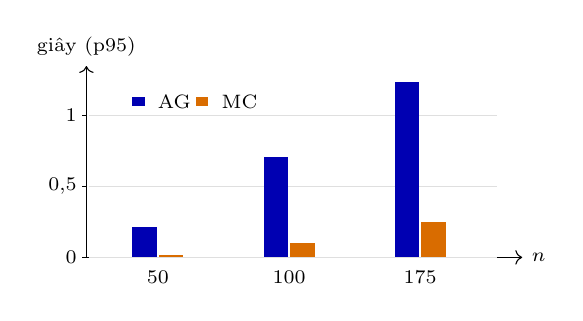
\begin{tikzpicture}[font=\scriptsize,scale=0.9]
\draw[->] (0.55,0.42)--(6.7,0.42) node[right] {$n$};
\draw[->] (0.55,0.42)--(0.55,3.12) node[above,align=center]{giây (p95)};
\foreach \y/\lab in {0.42/0,1.42/0{,}5,2.42/1}
  {\draw (0.49,\y)--(0.55,\y) node[left]{\lab};
   \draw[gray!25] (0.58,\y)--(6.35,\y);}
\fill[blue!70!black] (1.20,0.42) rectangle (1.55,0.846);
\fill[orange!85!black] (1.57,0.42) rectangle (1.92,0.458);
\fill[blue!70!black] (3.05,0.42) rectangle (3.40,1.838);
\fill[orange!85!black] (3.42,0.42) rectangle (3.77,0.622);
\fill[blue!70!black] (4.90,0.42) rectangle (5.25,2.888);
\fill[orange!85!black] (5.27,0.42) rectangle (5.62,0.914);
\node[below] at (1.56,0.36) {50};
\node[below] at (3.41,0.36) {100};
\node[below] at (5.26,0.36) {175};
\fill[blue!70!black] (1.20,2.55) rectangle (1.37,2.68);
\node[right] at (1.42,2.615) {AG};
\fill[orange!85!black] (2.10,2.55) rectangle (2.27,2.68);
\node[right] at (2.32,2.615) {MC};
\end{tikzpicture}
\ghichu{Phân vị 95 của thời gian giải mã hình học theo cỡ bài. AG và MC chạy trên hai máy Xeon khác tốc độ $\Rightarrow$ chỉ so xu hướng theo $n$ \textbf{trong từng bộ}, không so chiều cao giữa hai màu.}
\end{columns}
\end{frame}

%% ============================================================== Phụ lục K
\section{Phụ lục K: Phân tích mở rộng}

\begin{frame}[label=appK]{\apptitle{K}{Chi phí dừng và tính độc lập của dữ liệu kiểm tra}}
\begin{columns}[T,onlytextwidth]
\column{0.52\textwidth}
\scriptsize
\renewcommand{\arraystretch}{1.25}
\begin{tabular}{@{}lrrrrr@{}}
\toprule
$s^{\rm edge}/\tau$ & 0 & 0,05 & \cellcolor{hred!7}0,1 & 0,2 & 0,5\\\midrule
AG & 1,69 & 1,08 & \cellcolor{hred!7}0,75 & 0,42 & 0,12\\
MC & 2,41 & 1,78 & \cellcolor{hred!7}1,34 & 0,85 & 0,39\\
\bottomrule
\end{tabular}
\ghichu{Mức giảm $J$ (\%) của giải mã hình học so với chỉ tại nút trên cùng thứ tự, giải mã không giới hạn thời gian; cả hai phía được giải mã lại ở từng mức chi phí dừng. Đường cong mô tả của Hình 4, không phải phép so sánh chính mới.}
\vspace{4pt}
\begin{itemize}\scriptsize
\item Lợi ích còn lại giảm dần khi chi phí dừng tăng, nhưng \textbf{luôn dương} ở năm mức đã thử.
\end{itemize}
\column{0.45\textwidth}
\begin{block}{Tính độc lập của dữ liệu kiểm tra}
\scriptsize
\begin{itemize}
\item Bộ phát triển chỉ dùng để chọn \textbf{tập điểm, trần nhãn và phần thời gian dự trữ}; kết quả trên bộ này không được cộng vào ước lượng của AG hay MC.
\item Trước khi sinh MC: bộ giải mã hình học, cấu hình tìm kiếm với khởi tạo trực tiếp, tham số, seed và quy trình thống kê của phép so sánh này \textbf{đã được cố định}.
\item Kiểm tra trùng lặp: không có bộ tọa độ MC nào trong dữ liệu phát triển.
\item MC là dữ liệu mới cho đánh giá bộ giải mã tại thời điểm đó; GEMS hoàn chỉnh được đánh giá sau trên tập xác nhận 48 bộ riêng.
\end{itemize}
\end{block}
\end{columns}
\end{frame}

\begin{frame}{\apptitle{K}{Độ nhạy theo tham số vận hành}}
\begin{columns}[T,onlytextwidth]
\column{0.45\textwidth}
\scriptsize
\renewcommand{\arraystretch}{1.08}
\begin{tabular}{@{}lrr@{}}
\toprule
\textbf{Kịch bản} & $\delta$ & \textbf{Thắng/hòa}\\\midrule
\rowcolor{hred!7}Danh định & 0,82\% & 6/0\\
Pin $\times0{,}5$ & 2,44\% & 6/0\\
Pin $\times2$ & 0,56\% & 3/3\\
Sạc $\times0{,}5$ & 1,06\% & 6/0\\
Sạc $\times4$ & 1,52\% & 6/0\\
Hạn giao rộng & 1,68\% & 6/0\\
Hạn giao theo tuyến tham chiếu & 0,65\% & 6/0\\
Hạn giao chặt & 0,96\% & 6/0\\
Mọi khách được giao bằng UAV & 1,35\% & 6/0\\
Vùng dừng 50\% cạnh & 0,72\% & 6/0\\
Vùng dừng thưa & 0,44\% & 6/0\\
UAV hạ cánh chờ & 0,78\% & 6/0\\
Pin $\times0{,}5$, sạc $\times0{,}5$ & 1,84\% & 6/0\\
Pin $\times0{,}5$, sạc $\times4$ & 3,27\% & 6/0\\
\bottomrule
\end{tabular}
\column{0.52\textwidth}
\ghichu{Sáu bộ tọa độ, $n=100$, $\alpha=3$, một seed; hai cách giải mã chấm trong cùng kịch bản. $\delta$: mức giảm $J$ của giải mã hình học so với chỉ tại nút. Phép thăm dò: KTC từ sáu bộ tọa độ không dùng để khẳng định khả năng tổng quát.}
\vspace{4pt}
\begin{itemize}\scriptsize
\item 13 kịch bản về pin, sạc, hạn giao, vùng dừng và thao tác, bên cạnh danh định: mức giảm \textbf{luôn dương}; cỡ mẫu nhỏ $\Rightarrow$ chỉ là phân tích độ nhạy.
\item \textbf{Pin giảm một nửa}: lợi ích \textbf{tăng rõ} (2,44\%; 3,27\% khi kèm sạc $\times4$).
\item \textbf{Pin tăng gấp đôi}: một số lần giải mã \textbf{vượt phần thời gian dự trữ} vì có nhiều phương án khả thi hơn (3/6 hòa).
\item \textbf{UAV hạ cánh chờ} thay vì bay treo: lợi ích của điểm gặp trên cạnh vẫn còn, nhưng các điều kiện của lập luận năng lượng (Phụ lục E) \textbf{không còn nguyên vẹn}.
\item Bảng tách nguồn tăng lợi ích với các trường hợp hiệu ứng bị giới hạn bởi thời gian giải mã.
\end{itemize}
\end{columns}
\end{frame}

%% ============================================================== Phụ lục L
\section{Phụ lục L: Cất cánh và thu hồi khi xe đang chạy}

\begin{frame}[label=appL]{\apptitle{L}{Mở rộng: cất cánh và thu hồi UAV khi xe đang chạy}}
\begin{columns}[T,onlytextwidth]
\column{0.55\textwidth}
\begin{itemize}\scriptsize
\item Chi phí dừng làm giảm lợi ích của điểm gặp trên cạnh $\Rightarrow$ câu hỏi mở rộng: nếu UAV cất cánh/được thu hồi \textbf{khi xe vẫn đang chạy} thì lợi ích hình học có giữ được không?
\item Mô hình mở rộng: trong thời gian thao tác, xe đi với $\nu$ lần vận tốc thường và chịu thêm chi phí căn chỉnh $c_m$; ở điểm thu hồi khi xe đang chạy, UAV phải \textbf{có mặt đúng lúc} và xe không chờ.
\item Dữ liệu: \textbf{60 thứ tự} $n=175$ từ các lượt seed 1 của AG (hai tốc độ cho mỗi bộ tọa độ).
\item $\nu=0{,}5$, $c_m=0{,}05\tau$: giải mã có điểm trong cạnh giảm $J$ \textbf{4,55\%} so với chỉ tại nút (cùng trong mô hình xe đang chạy). $\nu=0{,}25$, $c_m=0{,}1\tau$: chỉ còn \textbf{1,54\%}; $\nu=1$: khoảng \textbf{8,7--8,9\%}.
\end{itemize}
\column{0.42\textwidth}
\centering
\small
\renewcommand{\arraystretch}{1.25}
\begin{tabular}{@{}rrr@{}}
\toprule
$\nu$ & $c_m/\tau$ & $\delta$\\\midrule
0,25 & 0,10 & 1,54\%\\
0,50 & 0,05 & 4,55\%\\
1,00 & 0,05 & 8,82\%\\
\bottomrule
\end{tabular}
\ghichu{Mô hình xe đang chạy trên 60 thứ tự AG: mức giảm $J$ so với chỉ tại nút, cùng chấm trong mô hình xe đang chạy. Thay $\nu$ hay $c_m$ là thay \textbf{kịch bản vật lý}, không phải phân tích thành phần của mô hình xe dừng giữa cạnh.}
\vspace{4pt}
\begin{alertblock}{Giới hạn}
\scriptsize $\nu$, $c_m$ chưa được đo từ thao tác thực; mô hình xe đang chạy thay đổi cả tập khả thi lẫn động học $\Rightarrow$ chỉ mô tả \textbf{độ nhạy}, không gộp với phép so sánh của mô hình xe dừng.
\end{alertblock}
\end{columns}
\end{frame}

%% ============================================================== Phụ lục M
\section{Phụ lục M: Đối chiếu trên TSP-D gốc}

\begin{frame}[label=appM]{\apptitle{M}{Makespan trên TSP-D gốc (1/2): họ đồng đều và một cụm}}
\scriptsize
\begin{center}
\renewcommand{\arraystretch}{1.12}
\setlength{\tabcolsep}{6pt}
\begin{tabular}{@{}lrrrrrrr@{}}
\toprule
\textbf{Họ} & $n$ & $\alpha$ & \shortstack{ICP\\công bố} & \shortstack{ICP\\chạy lại} & \shortstack{NICP\\chạy lại} & \shortstack{Tìm kiếm\\tại nút} & \shortstack{Chênh lệch\\so với ICP}\\\midrule
Đồng đều & 50 & 1 & 494,46 & 492,13 & 493,10 & 487,87 & $-0{,}88\%$\\
Đồng đều & 50 & 3 & 369,34 & 368,49 & 368,02 & 379,42 & $3{,}11\%$\\
Đồng đều & 100 & 1 & 649,31 & 650,59 & 652,09 & 661,01 & $1{,}61\%$\\
Đồng đều & 100 & 3 & 498,73 & 503,43 & 504,15 & 561,39 & $11{,}61\%$\\
Đồng đều & 175 & 1 & 830,11 & 832,62 & 833,67 & 852,05 & $2{,}35\%$\\
Đồng đều & 175 & 3 & 638,14 & 637,72 & 638,73 & 772,80 & $21{,}23\%$\\
\midrule
Một cụm & 50 & 1 & 654,15 & 654,24 & 654,24 & 631,00 & $-3{,}37\%$\\
Một cụm & 50 & 3 & 444,96 & 444,69 & 447,87 & 441,53 & $-0{,}56\%$\\
Một cụm & 100 & 1 & 1059,37 & 1057,50 & 1057,63 & 1070,18 & $1{,}26\%$\\
Một cụm & 100 & 3 & 727,54 & 726,42 & 730,17 & 845,08 & $16{,}42\%$\\
Một cụm & 175 & 1 & 1405,92 & 1406,26 & 1405,50 & 1436,99 & $2{,}21\%$\\
Một cụm & 175 & 3 & 989,47 & 992,56 & 989,75 & 1279,05 & $28{,}98\%$\\
\bottomrule
\end{tabular}
\end{center}
\ghichu{Makespan trên TSP-D gốc, trung bình 10 bài toán mỗi dòng (\textbf{không phải} mục tiêu $J$). ICP công bố: kết quả ICP v2; hai cột chạy lại dùng bản cài lại với tuyến Concorde phát hành cùng bộ dữ liệu; tìm kiếm tại nút chạy 10~s. Cột cuối: chênh lệch makespan của tìm kiếm tại nút so với ICP chạy lại, trung bình theo bài toán; dương nghĩa là tìm kiếm tại nút kém hơn. Khác tuyến khởi tạo và phần cứng $\Rightarrow$ không so trực tiếp thời gian công bố.}
\end{frame}

\begin{frame}{\apptitle{M}{Makespan trên TSP-D gốc (2/2): họ hai cụm và nhận xét}}
\scriptsize
\begin{center}
\renewcommand{\arraystretch}{1.12}
\setlength{\tabcolsep}{6pt}
\begin{tabular}{@{}lrrrrrrr@{}}
\toprule
\textbf{Họ} & $n$ & $\alpha$ & \shortstack{ICP\\công bố} & \shortstack{ICP\\chạy lại} & \shortstack{NICP\\chạy lại} & \shortstack{Tìm kiếm\\tại nút} & \shortstack{Chênh lệch\\so với ICP}\\\midrule
Hai cụm & 50 & 1 & 1002,50 & 1003,22 & 1003,11 & 984,33 & $-1{,}82\%$\\
Hai cụm & 50 & 3 & 731,92 & 733,04 & 736,64 & 730,01 & $-0{,}38\%$\\
Hai cụm & 100 & 1 & 1390,74 & 1385,83 & 1386,56 & 1408,24 & $1{,}63\%$\\
Hai cụm & 100 & 3 & 989,66 & 986,93 & 995,24 & 1123,32 & $13{,}87\%$\\
Hai cụm & 175 & 1 & 1896,14 & 1888,21 & 1892,25 & 1926,28 & $1{,}97\%$\\
Hai cụm & 175 & 3 & 1368,77 & 1364,82 & 1367,24 & 1730,83 & $26{,}93\%$\\
\bottomrule
\end{tabular}
\end{center}
\begin{columns}[T,onlytextwidth]
\column{0.49\textwidth}
\begin{block}{Bản cài lại ICP tái lập được số công bố}
\scriptsize Với tuyến khởi tạo LKH: lệch trung bình \textbf{0,04\%} so với trung bình nhóm của ICP v2. Cột ``ICP chạy lại'' dùng tuyến Concorde phát hành cùng dữ liệu: lệch trung bình (trị tuyệt đối) khoảng \textbf{0,25\%}.
\end{block}
\column{0.48\textwidth}
\begin{alertblock}{Tìm kiếm tại nút trên mục tiêu makespan}
\scriptsize Chạy 10~s: \textbf{kém ICP ở 13/18 nhóm}, kém giá trị công bố tốt nhất trong bảng của ICP v2 (gồm cả HGA-TAC$^+$, không in ở đây) ở \textbf{15/18 nhóm}, có nhóm tới \textbf{29\%}. Thuật toán tối ưu một mô hình khác $\Rightarrow$ \textbf{không} dùng để suy ra ưu thế trên $J$.
\end{alertblock}
\end{columns}
\end{frame}

\begin{frame}{\apptitle{M}{Nguồn số liệu và thông tin cần để tái lập}}
\begin{columns}[T,onlytextwidth]
\column{0.49\textwidth}
\begin{block}{Về các cột của bảng TSP-D gốc}
\scriptsize
\begin{itemize}
\item Thuộc \textbf{đợt tái hiện trước} đợt xác nhận.
\item Mã Julia gốc của ICP và HGA-TAC sau đó được chạy trên một tập con riêng (Phụ lục N); \textbf{không mặc định} mã HGA-TAC đó là biến thể HGA-TAC$^+$ trong mọi nguồn công bố.
\item Các nguồn HGA-TAC$^+$ có giá trị công bố không trùng nhau $\Rightarrow$ bảng chỉ dùng \textbf{một nguồn nhất quán} là ICP v2.
\item Phép so sánh sau chuyển đổi được báo riêng ở Bảng 2.
\end{itemize}
\end{block}
\column{0.48\textwidth}
\begin{block}{Một lượt chạy cần}
\scriptsize
\begin{itemize}
\item Tọa độ và tuyến tham chiếu, ma trận thời gian, thuộc tính khách, tham số năng lượng.
\item Seed tìm kiếm, thứ tự tại thời điểm dừng tìm kiếm, \textbf{mọi phương án đã hoàn tất} và thời gian đo thực tế.
\item Phương án đầu ra đánh giá lại từ tuyến xe, các khách UAV và các phân số cất cánh--thu hồi bằng \textbf{bộ đánh giá độc lập}.
\item Thống kê ghép cặp lấy \textbf{bộ tọa độ} làm đơn vị; hai tốc độ của cùng bộ ở cùng một cụm lấy mẫu.
\item Cấu hình máy, quy tắc thời gian, trường hợp không hoàn tất: Mục 5.3; công thức dựng bài toán: Phụ lục B.
\end{itemize}
\end{block}
\end{columns}
\end{frame}
%% ============================================================== Phụ lục N
\section{Phụ lục N: Thiết lập đối chứng và phân tích bổ sung}

\begin{frame}[label=appN]{\apptitle{N}{Phát triển phương pháp và chẩn đoán trên dữ liệu đã xem}}
\begin{columns}[T,onlytextwidth]
\column{0.50\textwidth}
\begin{block}{Tách ba giai đoạn}
\scriptsize
\begin{itemize}
\item Phụ lục tách \textbf{dữ liệu phát triển}, \textbf{việc chọn cấu hình} và \textbf{phần xác nhận} của GEMS; tên trong tệp kết quả đối chiếu ở Phụ lục T.
\item Đối chứng khởi tạo trực tiếp giữ các lựa chọn thuật toán của \textbf{đợt đánh giá trước} (AG và MC), cùng một bản sửa chung về cách kiểm tra giới hạn thời gian; mã đợt trước được lưu để \textbf{kiểm thử hồi quy}.
\item Các phép tách, mô phỏng và LNS \textbf{trùng với bản cũ} trên 20 ca khi không bị giới hạn thời gian cắt ngang.
\end{itemize}
\end{block}
\begin{alertblock}{Multi-start so với khởi tạo trực tiếp}
\scriptsize Trên dữ liệu phát triển: multi-start cho $J$ thấp hơn \textbf{1,49\%} ở 30~s (hai seed; 8 cấu hình tốt hơn, 3 kém). Trên tập xác nhận ở 60~s: chỉ còn \textbf{0,47\%} (KTC [$-0{,}22$; 1,21]; 22 bộ tốt hơn, 2 hòa, 24 kém). Chênh lệch có thể do khác thời gian chạy (30 so với 60~s), do ước lượng trên dữ liệu phát triển lạc quan, hoặc cả hai --- dữ liệu hiện có \textbf{chưa tách được}.
\end{alertblock}
\column{0.47\textwidth}
\begin{block}{Chẩn đoán trên 12 cấu hình phát triển (có cộng thêm thời gian)}
\scriptsize
\renewcommand{\arraystretch}{1.2}
\begin{tabularx}{\linewidth}{@{}Yr@{}}
\toprule
\textbf{Thay đổi thử} & \textbf{Mức giảm $J$}\\\midrule
Giải mã thêm 16 thứ tự tốt hoặc đa dạng của quần thể & 0,10\%\\
Tìm kiếm theo cửa sổ 6 / 10 / 14 khách, thêm 5~s & 0,19 / 0,18 / 0,08\%\\
LNS trực tiếp trên mô hình dừng giữa cạnh, thêm 5~s & 0,50\%\\
\bottomrule
\end{tabularx}
\vspace{2pt}
Đây là chẩn đoán \textbf{có cộng thêm thời gian}, không phải so sánh cùng ngân sách. Các mức lợi nhỏ dẫn tới quyết định \textbf{ưu tiên chia thời gian giữa multi-start và quần thể}, dù chưa loại trừ khả năng một thiết kế tìm kiếm hình học khác hiệu quả hơn.
\end{block}
\end{columns}
\end{frame}

\begin{frame}{\apptitle{N}{Hai bản chuyển đổi HGA-J và ICP-J}}
\begin{columns}[T,onlytextwidth]
\column{0.49\textwidth}
\begin{block}{HGA-J}
\scriptsize
\begin{itemize}
\item Mã toán tử của HGA-TAC tại commit \texttt{8f1f345c}; hàm đánh giá thay bằng \textbf{phép tách có giữ loại phương tiện} và kiểm tra pin theo chuỗi.
\item Các cấu hình khởi tạo, độ rộng lân cận, quần thể và trần nhãn thử trên dữ liệu phát triển; bản được chọn: \textbf{quần thể tối thiểu 8, bổ sung 12 cá thể, trần 64 nhãn}.
\end{itemize}
\end{block}
\begin{block}{ICP-J}
\scriptsize
\begin{itemize}
\item Đoạn tối đa \textbf{20 nút}, trần \textbf{32 nhãn}; khởi tạo bằng thứ tự kiến tạo tốt nhất; \textbf{khởi động lại} từ thứ tự kế tiếp khi còn thời gian.
\item Khi bộ nhớ đệm có thứ tự đề xuất cho cùng một đoạn: giải mã lại thứ tự đó từ trạng thái thời gian--pin hiện tại, \textbf{không chạy lại} tìm kiếm thứ tự trong đoạn; QHĐ vẫn chọn lại phương án phối hợp cho thứ tự đã lưu.
\end{itemize}
\end{block}
\column{0.48\textwidth}
\begin{block}{Kiểm tra}
\scriptsize
\begin{itemize}
\item Phép tách có giữ loại phương tiện: phát lại trên \textbf{450 nhiễm sắc thể} ngẫu nhiên (sai lệch tối đa $\approx9\cdot10^{-16}$) và vét cạn trên \textbf{176 ca nhỏ} ($\approx6\cdot10^{-16}$).
\item ICP-J: đánh giá lại toàn bộ lịch sau mỗi thay đổi; chạy lặp trên ca nhỏ tới hội tụ.
\item Các phép kiểm tra khi \textbf{tắt UAV}, \textbf{nới hạn giao} và \textbf{sắp ưu tiên theo hàm đánh giá} cũng đạt.
\end{itemize}
\end{block}
\begin{alertblock}{Diễn giải}
\scriptsize Hai bản chuyển đổi là các \textbf{đối chứng được mô tả cụ thể}, không phải bằng chứng về chất lượng tốt nhất mà họ phương pháp này có thể đạt. Kiểm tra xác nhận các hành vi đã kiểm, \textbf{không thay thế} việc đánh giá độ mạnh của toán tử hay độ biến thiên khi bị giới hạn thời gian cắt ngang.
\end{alertblock}
\end{columns}
\end{frame}

\begin{frame}{\apptitle{N}{Tập chọn cấu hình và giao thức chạy}}
\begin{columns}[T,onlytextwidth]
\column{0.50\textwidth}
\begin{block}{Tập chọn cấu hình (12 bộ mới, một seed)}
\scriptsize GEMS được đối chiếu với \textbf{multi-start phân bổ thời gian thích nghi}: bốn lượt LNS trong nửa đầu ngân sách, giữ hai lượt tốt hơn chạy tiếp trong một phần tư, phần còn lại cho lượt tốt nhất.
\vspace{3pt}

\renewcommand{\arraystretch}{1.15}
\begin{tabular}{@{}lr@{}}
\toprule
\textbf{Phương pháp} & $J$ \textbf{trung bình}\\\midrule
\rowcolor{hred!7}GEMS & 1,5713\\
Multi-start phân bổ thích nghi & 1,5723\\
ICP-J & 2,1624\\
HGA-J & 2,1796\\
\bottomrule
\end{tabular}
\vspace{3pt}
\begin{itemize}
\item GEMS và ICP-J được chọn theo quy tắc $J$ trung bình \textbf{định trước}; nếu dùng trung bình tỷ số so với khởi tạo trực tiếp, \textbf{thứ tự của cả hai cặp đảo lại}.
\item Biến thể multi-start thích nghi \textbf{chưa chạy} trên tập xác nhận $\Rightarrow$ \textbf{không kết luận} GEMS tốt hơn biến thể này.
\end{itemize}
\end{block}
\column{0.47\textwidth}
\begin{block}{Giao thức chạy đợt xác nhận}
\scriptsize
\begin{itemize}
\item Xeon 2,8~GHz hai lõi, 8~GB RAM; hai tiến trình một luồng chạy song song.
\item Môi trường khởi động trước khi đo; thời gian biên dịch JIT của Julia (HGA-J) ghi riêng.
\item Khởi tạo riêng của từng phương pháp, tìm kiếm và giải mã đều nằm trong \textbf{60~s}.
\item \textbf{Tám lượt} bị ảnh hưởng bởi tác vụ phụ được chạy lại; bản cũ giữ để kiểm tra độ nhạy.
\item Không lượt nào có tổng thời gian giải ghi nhận vượt 60~s; mọi lời giải cuối khớp bộ đánh giá Python độc lập, sai lệch tương đối lớn nhất $\approx10^{-15}$.
\end{itemize}
\end{block}
\end{columns}
\end{frame}

\begin{frame}{\apptitle{N}{Biến thiên trên tập xác nhận và giới hạn diễn giải}}
\begin{columns}[T,onlytextwidth]
\column{0.50\textwidth}
\begin{block}{Biến thiên (GEMS so với khởi tạo trực tiếp)}
\scriptsize
\begin{itemize}
\item Theo cỡ: $-0{,}03$\%, 0,85\% và 2,43\% ở $n=50,100,175$.
\item Trung vị trên 48 bộ: \textbf{0,02\%}; \textbf{toàn bộ 12 trường hợp hòa} thuộc cỡ 50; mức giảm lớn nhất \textbf{8,71\%}.
\item Lát cắt \textbf{mô tả}, không phải các phép kiểm độc lập.
\end{itemize}
\end{block}
\begin{block}{Đối chứng khởi tạo trực tiếp so với hai bản chuyển đổi}
\scriptsize Giảm $J$ \textbf{25,15\%} so với HGA-J và \textbf{23,26\%} so với ICP-J. Các khoảng cách thuộc phép so sánh với bản chuyển đổi dưới bộ giải mã chung, \textbf{không đo} phần cải thiện do cách khởi tạo và phân bổ thời gian.
\end{block}
\column{0.47\textwidth}
\begin{alertblock}{Chưa tách được}
\scriptsize
\begin{itemize}
\item Phép so sánh GEMS với khởi tạo trực tiếp và multi-start đánh giá \textbf{toàn bộ cách kết hợp}.
\item Thực nghiệm chưa tách riêng tác động của \textbf{chuyển lời giải sang quần thể} khỏi tác động của \textbf{lịch chia thời gian}.
\item \textbf{Chưa đánh giá GEMS khi bỏ sàng lọc}.
\item $\Rightarrow$ mức giảm \textbf{1,08\%} không được gán riêng cho một trong các thành phần đó.
\end{itemize}
\end{alertblock}
\end{columns}
\end{frame}

\begin{frame}{\apptitle{N}{Phân tích thành phần và độ nhạy trên tập con xác nhận}}
\begin{columns}[T,onlytextwidth]
\column{0.53\textwidth}
\scriptsize
\renewcommand{\arraystretch}{1.25}
\begin{tabularx}{\linewidth}{@{}Yrr@{}}
\toprule
\textbf{So sánh} & $\delta$ (\%) & \textbf{KTC 95\%}\\
\midrule
$K=16$ so với $K=1$, giải mã chỉ tại nút & $-0{,}89$ & $[-1{,}79;-0{,}15]$\\
$K=16$ so với $K=1$, giải mã hình học & $-0{,}74$ & $[-1{,}65;0{,}03]$\\
Hình học so với chỉ tại nút, $K=1$ & 0,63 & $[0{,}33;1{,}01]$\\
Hình học so với chỉ tại nút, $K=16$ & 0,78 & $[0{,}43;1{,}20]$\\
\bottomrule
\end{tabularx}
\ghichu{Khởi tạo trực tiếp trên 12 bộ tọa độ của tập xác nhận, ba seed. $\delta>0$: cấu hình đứng trước có $J$ thấp hơn cấu hình đứng sau.}
\vspace{3pt}
\begin{itemize}
\item Bản không sàng lọc dùng $K=1$; mỗi lượt tìm kiếm được giải mã theo hai cách (chỉ tại nút; chỉ tại nút rồi hình học); bản có sàng lọc dùng lại các lượt khởi tạo trực tiếp của phép so sánh chính.
\item Hai cách giải mã nhận \textbf{cùng thứ tự và cùng mốc dừng} $\Rightarrow$ đo hiệu ứng giải mã trên cùng một kết quả tìm kiếm, không đo việc dành toàn bộ thời gian dự trữ cho tìm kiếm tại nút.
\end{itemize}
\column{0.44\textwidth}
\begin{block}{GEMS so với khởi tạo trực tiếp trên tập con}
\scriptsize
\begin{itemize}
\item Danh định: \textbf{0,49\%} (KTC [$-0{,}36$; 1,74], ba seed) --- thấp hơn mức trung bình toàn tập xác nhận; hai seed như phân tích độ nhạy: 0,62\%.
\item \textbf{Pin} (dung lượng và dự trữ) giảm một nửa: GEMS có $J$ \textbf{cao hơn} 0,19\% (KTC của mức giảm [$-1{,}43$; 0,86]).
\item \textbf{Dừng $0{,}5\tau$} mỗi phía: mức giảm 0,41\% ([$-0{,}78$; 1,96]).
\end{itemize}
\end{block}
\begin{alertblock}{Kết luận thận trọng}
\scriptsize Chưa có bằng chứng rõ GEMS tốt hơn trong hai kịch bản này; cũng \textbf{chưa đủ} để kết luận thay đổi tham số làm mất lợi ích, vì ngay ở kịch bản danh định trên tập con, KTC cũng chứa 0.
\end{alertblock}
\end{columns}
\end{frame}

\begin{frame}{\apptitle{N}{Thời gian đạt ngưỡng và giới hạn diễn giải}}
\begin{columns}[T,onlytextwidth]
\column{0.50\textwidth}
\begin{block}{Chỉ số đã khóa trước}
\scriptsize
\begin{itemize}
\item Ngưỡng: $J$ cuối cùng của bước tìm kiếm tại nút của \textbf{đối chứng} (cùng seed); đo thời gian $t^{\rm hit}_{\rm GEMS}$ để GEMS lần đầu đạt ngưỡng.
\item Tỷ số báo cáo: $t^{\rm end}_{\rm ĐC}/t^{\rm hit}_{\rm GEMS}$, tử số là toàn bộ thời gian tìm kiếm thực dùng của đối chứng.
\item Mỗi bộ tọa độ lấy trung vị qua seed; lượt không đạt ngưỡng gán tỷ số 0.
\item So với khởi tạo trực tiếp: trung vị theo bộ tọa độ \textbf{2,24}; \textbf{56\%} bộ có tỷ số $\ge2$; ở \textbf{19\%} bộ, GEMS không đạt ngưỡng trong 60~s.
\end{itemize}
\end{block}
\column{0.47\textwidth}
\begin{alertblock}{Vì sao không kết luận ``nhanh gấp đôi''}
\scriptsize
\begin{itemize}
\item Chỉ số đo thời gian để đạt \textbf{chất lượng cuối} của đối chứng, chưa phải tỷ số giữa hai thời gian đạt cùng một ngưỡng: đối chứng có thể đã đạt ngưỡng sớm rồi chạy tiếp mà không cải thiện.
\item Phân tích \emph{post hoc} trên chính các vết đã lưu, thay tử số bằng thời điểm đối chứng \textbf{lần đầu đạt} ngưỡng của nó: trung vị chỉ còn \textbf{0,96} (so với khởi tạo trực tiếp) và \textbf{1,28} (so với multi-start); khoảng \textbf{21\%} bộ có tỷ số $\ge2$ trong mỗi phép.
\item Phép này cũng phụ thuộc ngưỡng lấy từ đối chứng và chỉ xét tìm kiếm tại nút, chưa gồm giải mã cuối $\Rightarrow$ \textbf{không kết luận} GEMS tăng tốc cả phương pháp gấp đôi.
\end{itemize}
\end{alertblock}
\end{columns}
\end{frame}

\begin{frame}{\apptitle{N}{Chạy mã gốc trên TSP-D gốc}}
\begin{columns}[T,onlytextwidth]
\column{0.50\textwidth}
\scriptsize
\renewcommand{\arraystretch}{1.05}
\begin{tabular}{@{}lrrrrr@{}}
\toprule
\textbf{Họ} & $n$ & $\alpha$ & \shortstack{HGA-\\TAC} & \shortstack{memetic\\tại nút} & \shortstack{ICP\\(mã gốc)}\\
\midrule
Đồng đều & 100 & 1 & 688,51 & 678,40 & 671,47\\
Đồng đều & 100 & 3 & 524,20 & 563,51 & 518,17\\
Đồng đều & 175 & 1 & 858,10 & 866,13 & 858,62\\
Đồng đều & 175 & 3 & 681,85 & 751,39 & 649,39\\
Một cụm & 100 & 1 & 1012,75 & 1017,18 & 1017,66\\
Một cụm & 100 & 3 & 743,82 & 743,64 & 711,86\\
Một cụm & 175 & 1 & 1368,18 & 1394,81 & 1343,45\\
Một cụm & 175 & 3 & 1007,41 & 1113,65 & 938,12\\
Hai cụm & 100 & 1 & 1349,36 & 1335,80 & 1339,06\\
Hai cụm & 100 & 3 & 963,04 & 998,40 & 922,31\\
Hai cụm & 175 & 1 & 1666,97 & 1675,89 & 1687,40\\
Hai cụm & 175 & 3 & 1264,49 & 1347,12 & 1195,04\\
\bottomrule
\end{tabular}
\ghichu{Makespan (không phải $J$). Mã số bài toán: 91 ở $n=100$, 101 ở $n=175$ cho mỗi họ. HGA-TAC và memetic tại nút: trung bình hai seed.}
\column{0.47\textwidth}
\begin{itemize}\scriptsize
\item 12 cấu hình Agatz: ba họ, cỡ 100 và 175, tốc độ 1 và 3; memetic tại nút với khởi tạo trực tiếp và \textbf{mã gốc} của hai phương pháp TSP-D.
\item ICP: một lượt tới hội tụ với tuyến Concorde phát hành cùng dữ liệu; hội tụ trong \textbf{0,3--12,3~s}.
\item HGA-TAC giữ điều kiện dừng của tác giả với trần 60~s: \textbf{17/24 lượt dừng sớm} sau 16,5--55,7~s; bảy lượt còn lại bị trần cắt, chỉ lời giải tốt nhất trước mốc 60~s được tính. Memetic dùng đủ thời gian $\Rightarrow$ \textbf{không} phải so sánh cùng thời gian thực.
\item Mã gốc ICP tại commit \texttt{becd5aa9} cho \textbf{cùng giá trị} với bản cài lại khi dùng cùng tuyến khởi tạo, trên 12 cấu hình và một ca bổ sung có giới hạn tầm bay; ở ca đó, hàm đánh giá của HGA-TAC báo giá trị khác với giá trị phát lại $\Rightarrow$ dùng \textbf{giá trị phát lại}.
\item Memetic tại nút có makespan cao hơn ICP trung bình \textbf{0,79\%} khi $\alpha=1$ và \textbf{11,43\%} khi $\alpha=3$. Đảo thứ hạng giữa mô hình gốc và mô hình $J$ \textbf{không cô lập được} ảnh hưởng của mục tiêu khỏi ảnh hưởng của bản chuyển đổi và ngân sách thời gian.
\end{itemize}
\end{columns}
\end{frame}

\begin{frame}{\apptitle{N}{Dữ liệu và tái lập (đợt E23)}}
\scriptsize Đường dẫn tính từ thư mục \path{uavgv_exp_cloud/}.
\vspace{4pt}

\renewcommand{\arraystretch}{1.3}
\begin{tabularx}{\textwidth}{@{}P{4.2cm}Y@{}}
\toprule
\textbf{Nội dung} & \textbf{Tệp / thư mục}\\\midrule
Cấu hình và mã băm của mã nguồn & \path{results/e23_lock.json}, \path{results/e23_manifest.json}\\
Dữ liệu dẫn xuất & \path{benchmark/e23_derived/}\\
Dữ liệu thô & \path{results/e23_runs_C2_*.json}, \path{results/e23_runs_M_*.json}, \path{results/e23_runs_R_*.json}, \path{results/e23_native/}\\
Script tạo các bảng chính & \path{experiments/analyze_e23.py}\\
Mã GEMS; các bản chuyển đổi & \path{uavgv/gems23.py}; \path{cpp/e23_ext.hpp} và \path{scripts/sota_native_julia/e23/hgaj/}\\
Thời gian đạt ngưỡng (post hoc) & trường \texttt{trace\_t}, \texttt{trace\_J}, \texttt{J\_node} --- tách khỏi chỉ số đã khóa\\
Lượt bị ảnh hưởng bởi tác vụ phụ & \path{results/e23_runs_C2_disturbed.json}: thay kết quả chạy lại bằng lượt cũ vẫn cho mức giảm của GEMS so với khởi tạo trực tiếp $\approx$ \textbf{1,082\%}\\
Sửa đổi script phân tích sau khi khóa & \path{results/e23_patches.jsonl}; mã băm giữ để phân biệt sửa cách trình bày với thay đổi phương pháp\\
\bottomrule
\end{tabularx}
\end{frame}
%% ============================================================== Phụ lục O
\section{Phụ lục O: Tham số các khảo sát tìm thứ tự}

\begin{frame}[label=appO]{\apptitle{O}{Tham số tầng tìm kiếm và các đối chứng}}
\scriptsize
\renewcommand{\arraystretch}{1.08}
\begin{tabularx}{\textwidth}{@{}YP{6.6cm}@{}}
\toprule
\textbf{Tham số} & \textbf{Giá trị}\\
\midrule
Quy mô quần thể; số cá thể con giữa hai lần thu gọn & 12; 20\\
Số cá thể được bảo vệ; số cá thể gần nhất dùng để đo tính đa dạng & 4; 3\\
Số cá thể con từ mỗi cặp bố mẹ $K$ & 16 (\unscreened{}: 1)\\
Giải mã khi sàng lọc & $L=8$, $h=12$\\
Giải mã trước tìm kiếm cục bộ & $L=64$, $h=12$\\
Tìm kiếm cục bộ: số vòng LNS; khoảng nhiệt độ & 100; $0{,}05\to0{,}005$\\
Số khách hàng tạm loại mỗi vòng LNS & 3 hoặc 8 (\lnsq{}, \msl{}, \msd{}, \mth{ILS}: 3 hoặc 16)\\
Giới hạn lượt bay khi chèn trong LNS & Điểm cất cánh và thu hồi cách nhau tối đa 5 vị trí trên tuyến xe\\
Giải mã lại trong LNS & $L=8$, $h=12$\\
LNS chạy độc lập: nhiệt độ & $0{,}5\to0{,}005$\\
Điều kiện tăng tính đa dạng & Sau 128 cá thể con không cải thiện $z^{*}$; giữ lại 4 cá thể\\
Tham số $\theta$ của chỉ số ATC & 0,5; 2; 8; 32; $\infty$\\
Xáo trộn khi khởi tạo & 4 lần di chuyển hoặc đảo đoạn, dài tối đa $m/8$ khách hàng\\
Đột biến (memetic đột biến) & 2 lần di chuyển hoặc đảo đoạn, dài tối đa $m/8$ khách hàng\\
Đột biến nhỏ (\smallmutation{}, memetic đột biến nhỏ với khởi tạo đa dạng) & 1 lần di chuyển hoặc đảo đoạn, dài tối đa 6 khách hàng\\
Multi-start & 4 lần chạy, mỗi lần dùng 1/4 tổng thời gian\\
Seed của bộ sinh số ngẫu nhiên & 1 và 2\\
\bottomrule
\end{tabularx}
\ghichu{Cấu hình của các khảo sát tại nút. Hai seed thuộc khảo sát sàng lọc; các phép so sánh trên AG và MC dùng ba seed (Mục 5).}
\end{frame}

%% ============================================================== Phụ lục P
\section{Phụ lục P: Thiết kế các khảo sát tìm thứ tự}

\begin{frame}[label=appP]{\apptitle{P}{Dữ liệu và kịch bản khẩn cấp của các khảo sát}}
\footnotesize Bốn khảo sát về lựa chọn cá thể, khởi tạo và cấu trúc lời giải; \textbf{chỉ xét điểm gặp tại nút}. Các biến thể memetic khởi tạo trực tiếp từ thứ tự kiến tạo: phân tích các thành phần dùng chung trong pha quần thể, \textbf{không thay thế} phép đánh giá GEMS hoàn chỉnh. Mã lưu trữ: Phụ lục T.
\begin{columns}[T,onlytextwidth]
\column{0.50\textwidth}
\begin{block}{Dữ liệu (TSP-D công khai + kịch bản chung)}
\scriptsize Giữ nguyên tọa độ và thời gian di chuyển; thêm hạn giao, trọng số ưu tiên và tham số năng lượng.
\begin{itemize}
\item \textbf{N100}: bài 99 hoặc 100 khách --- bộ Random và Amsterdam của Bogyrbayeva và cs.~\cite{bogyrbayeva2023} và bộ của Ha và cs.~\cite{ha2020}.
\item \textbf{N175}: bài 174 khách của Agatz và cs.~\cite{agatz2018} (uniform, singlecenter, doublecenter), UAV \textbf{nhanh gấp đôi} xe.
\item 30\% khách khẩn ($w_i=5$), còn lại $w_i=1$; khoảng 80\% khách được giao bằng UAV (giữ nguyên nếu bộ gốc đã quy định).
\item Dữ liệu ngẫu nhiên sinh từ seed cố định theo tên bài $\Rightarrow$ mọi thuật toán nhận cùng đầu vào.
\end{itemize}
\end{block}
\column{0.47\textwidth}
\begin{block}{Hạn giao}
\scriptsize
\[
d_i=\tT_{0i}+\eta_i\,\Mref,
\]
thời gian xe đi thẳng từ kho cộng một độ dư tỷ lệ với makespan tuyến tham chiếu; $\eta_i\sim U[0{,}05;\,0{,}25]$ (khẩn), $U[0{,}5;\,1{,}0]$ (thường) --- chính là công thức của AG với $\gamma=1$, $s^{\rm T}_i=0$. Với cách đặt này, \textbf{mọi phương án tìm được đều có khách trễ} ($\meanT>0$) $\Rightarrow$ phải cân nhắc thứ tự ưu tiên.
\end{block}
\begin{block}{Tham số năng lượng}
\scriptsize $P\sub{ce}=1$ (đơn vị); $P\sub{cl}=1{,}3$, $P\sub{hv}=1{,}2$, $P\sub{sv}=1{,}56$, $P\sub{to}=2{,}028$, $P\sub{ld}=1{,}2$; $t\sub{to}=t\sub{ld}=t\sub{sv}=0{,}1\tau$, $s_L=s_R=0{,}15\tau$, $s^{\rm T}_i=0$; $B=12\tau$ (đủ bay không tải 12 đơn vị thời gian), $b_{\min}=0{,}1B$, $r_c=0{,}5$. Kịch bản chuẩn hóa, \textbf{không phải} thông số đo của một mẫu UAV cụ thể.
\end{block}
\end{columns}
\end{frame}

\begin{frame}{\apptitle{P}{Phương pháp được so sánh (1/2): khảo sát khởi tạo}}
\scriptsize
\renewcommand{\arraystretch}{1.08}
\begin{tabularx}{\textwidth}{@{}P{3.0cm}YP{2.0cm}@{}}
\toprule
\textbf{Cách tìm kiếm} & \textbf{Mô tả} & \textbf{Khởi tạo}\\
\midrule
\lns{} & Chạy LNS trong toàn bộ thời gian; mỗi vòng loại 3 hoặc 8 khách. Đây là mốc so sánh. & Tham chiếu\\
\lnsq{} & Như LNS, nhưng mỗi vòng loại 3 hoặc 16 khách. & Tham chiếu\\
\msl{} & Chạy LNS mở rộng độc lập bốn lần, chia đều ngân sách và lấy lời giải tốt nhất. & Tham chiếu\\
\msd{}$^{\dagger}$ & Bốn lượt LNS từ bốn thứ tự có điểm giải mã tốt nhất. Cũng được dùng trong khảo sát sàng lọc. & Đa dạng\\
\mth{ILS} & Xáo trộn thứ tự, giải mã và cải thiện; chỉ chấp nhận lời giải tốt hơn. & Tham chiếu\\
Memetic, đột biến & Tạo cá thể con bằng hai lần di chuyển hoặc đảo đoạn, mỗi đoạn dài tối đa $m/8$; dùng $K=1$. & Tham chiếu hoặc đa dạng\\
Memetic, lai ghép & Dùng LOX để tạo cá thể con, với $K=1$. & Tham chiếu hoặc đa dạng\\
Memetic, đột biến nhỏ$^{\dagger}$ & Một lần di chuyển hoặc đảo đoạn dài tối đa sáu khách; chỉ khảo sát ở nhóm N175. & Đa dạng\\
\bottomrule
\end{tabularx}
\ghichu{Khởi tạo ``đa dạng'' dùng sáu thứ tự ở Phụ lục D; ``tham chiếu'' dùng tuyến LKH. Dấu $\dagger$: đối chứng bổ sung sau khi xem kết quả khảo sát khởi tạo.}
\vspace{6pt}
\begin{block}{Điểm chung và một khác biệt cần lưu ý}
\scriptsize Mọi phương pháp dùng chung \textbf{mô hình đánh giá, bộ giải mã và thủ tục LNS}; khác biệt chính là \textbf{cách khởi tạo} và \textbf{cách tổ chức tìm kiếm}. Riêng cấu hình giải mã ban đầu: \lns{} và các phương pháp multi-start dùng $L=8$, còn các thuật toán memetic dùng $L=64$.
\end{block}
\end{frame}

\begin{frame}{\apptitle{P}{Phương pháp được so sánh (2/2): khảo sát sàng lọc}}
\scriptsize
\renewcommand{\arraystretch}{1.2}
\begin{tabularx}{\textwidth}{@{}P{3.0cm}YP{2.0cm}@{}}
\toprule
\textbf{Cách tìm kiếm} & \textbf{Mô tả} & \textbf{Khởi tạo}\\
\midrule
\unscreened{} & Tạo một cá thể bằng LOX rồi cải thiện bằng LNS. Cũng dùng để lấy quần thể cho khảo sát xếp hạng cá thể. & Đa dạng\\
\randomchild{} & Tạo và giải mã 16 cá thể bằng LOX, chọn ngẫu nhiên một cá thể để chạy LNS. & Đa dạng\\
\smallmutation{} & Tạo 16 cá thể bằng đột biến nhỏ từ một bố hoặc mẹ; chọn theo điểm giải mã. & Đa dạng\\
\rowcolor{hred!7}\screened{} & Tạo 16 cá thể bằng LOX, chọn cá thể có $\Jhat$ nhỏ nhất để chạy LNS. & Đa dạng\\
\bottomrule
\end{tabularx}
\ghichu{\msd{} (bảng trước) cũng được chạy trên dữ liệu khảo sát sàng lọc.}
\vspace{6pt}
\begin{columns}[T,onlytextwidth]
\column{0.49\textwidth}
\begin{block}{Ba đối chứng thành phần của bản có sàng lọc}
\scriptsize
\begin{itemize}
\item \unscreened{}: \textbf{không sàng lọc} ($K=1$).
\item \randomchild{}: vẫn \textbf{giải mã mọi cá thể con} nhưng chọn ngẫu nhiên thay vì theo giá trị giải mã.
\item \smallmutation{}: tạo cá thể con bằng \textbf{đột biến thay cho lai ghép}.
\end{itemize}
\end{block}
\column{0.48\textwidth}
\begin{block}{Đối chứng không duy trì quần thể}
\scriptsize Ngoài ra, \msd{} là đối chứng \textbf{không duy trì quần thể}: bốn lượt LNS độc lập từ bốn thứ tự xuất phát khác nhau, lấy lời giải tốt nhất.
\end{block}
\end{columns}
\end{frame}

\begin{frame}{\apptitle{P}{Quy trình bốn khảo sát và cách tổng hợp kết quả}}
\scriptsize
\renewcommand{\arraystretch}{1.05}
\begin{tabularx}{\textwidth}{@{}P{1.9cm}P{3.9cm}P{3.3cm}Y@{}}
\toprule
\textbf{Khảo sát} & \textbf{Câu hỏi nghiên cứu} & \textbf{Dữ liệu} & \textbf{Nội dung đánh giá}\\
\midrule
Sàng lọc & Sàng lọc có cải thiện lời giải cuối cùng trong cùng thời gian? & 12 bài toán N175 mới & $J$ cuối cùng sau 15 và 60~s\\
Xếp hạng cá thể & Điểm giải mã dự báo chất lượng sau tìm kiếm cục bộ tốt đến đâu? & 4 bài N175 khác; 48 cặp bố mẹ, mỗi cặp tạo 16 cá thể con & Chạy tìm kiếm cục bộ cho mỗi cá thể con hai lần độc lập, ngoài quá trình tìm kiếm\\
Khởi tạo & Cách tổ chức tìm kiếm nào cho $J$ nhỏ nhất trong cùng thời gian? & 12 bài N100 và 12 bài N175 & $J$ cuối cùng sau 10 và 40~s (N100), 15 và 60~s (N175)\\
Cấu trúc lời giải & Thành phần nào tạo nên chênh lệch chất lượng lời giải? & Lời giải cuối cùng của khảo sát khởi tạo & Phân tích chênh lệch $J$ giữa lời giải của \lns{} và lời giải tốt nhất\\
\bottomrule
\end{tabularx}
\ghichu{Câu hỏi và thiết kế của các khảo sát bước tìm thứ tự. Mỗi cấu hình chạy với hai seed.}
\vspace{1pt}
\begin{columns}[T,onlytextwidth]
\column{0.42\textwidth}
\begin{block}{Cách tổng hợp kết quả}
\scriptsize $\bar J_{a,i}$: trung bình $J$ hai seed của phương pháp $a$ trên bài $i$;
\[
\delta_i(a,b)=100\left(1-\frac{\bar J_{a,i}}{\bar J_{b,i}}\right)\ (\%),
\]
rồi trung bình trên 12 bài; $\delta_i>0$: $a$ tốt hơn $b$. KTC: \textbf{5.000} lần bootstrap theo bài, \textbf{chưa hiệu chỉnh} so sánh bội.
\end{block}
\column{0.55\textwidth}
\begin{block}{Trình tự}
\scriptsize Khảo sát khởi tạo và phân tích cấu trúc lời giải thực hiện \textbf{trước} để định hướng thiết kế phương pháp. Tiếp theo, khảo sát xếp hạng kiểm tra khả năng chọn cá thể bằng điểm giải mã, rồi khảo sát sàng lọc đánh giá tác động trong quá trình tìm kiếm. Hai khảo sát về cá thể dùng bài N175 chưa xuất hiện trong khảo sát khởi tạo; dữ liệu xếp hạng và dữ liệu sàng lọc \textbf{không trùng nhau}.
\end{block}
\end{columns}
\end{frame}

\begin{frame}{\apptitle{P}{Giới hạn thời gian, môi trường chạy, thống kê và ghi nhận trước}}
\begin{columns}[T,onlytextwidth]
\column{0.50\textwidth}
\begin{block}{Giới hạn thời gian}
\scriptsize
\begin{itemize}
\item Đồng hồ thực, gồm khởi tạo thứ tự, giải mã, sàng lọc và LNS; riêng tuyến tham chiếu tính trước và dùng chung.
\item N100: mốc \textbf{10~s và 40~s}; N175: \textbf{15~s và 60~s} (thời gian chạy ngắn và dài).
\item \lns{} và các phương pháp multi-start chạy \textbf{riêng ở từng mốc} (lịch giảm nhiệt phụ thuộc thời gian cho phép).
\item Phương pháp duy trì quần thể chạy tới mốc dài; kết quả mốc ngắn = lời giải tốt nhất tại thời điểm đó.
\end{itemize}
\end{block}
\begin{alertblock}{Ghi nhận trước và hậu kiểm}
\scriptsize Tham số LNS và quần thể chọn trước trên một tập bài tổng hợp riêng. Cấu hình tám phương pháp ban đầu (khảo sát khởi tạo) và bốn biến thể (khảo sát sàng lọc) \textbf{ghi nhận trước khi chạy}. Đối chứng $\dagger$ bổ sung sau khi xem kết quả khởi tạo; multi-start đánh giá thêm trên dữ liệu sàng lọc với cấu hình đã dùng $\Rightarrow$ các so sánh liên quan là \textbf{phân tích hậu kiểm}.
\end{alertblock}
\column{0.47\textwidth}
\begin{block}{Môi trường}
\scriptsize Bộ giải mã, LNS, mô hình đánh giá cài bằng C++, gọi từ Python~3.13; một luồng; Linux, Intel Xeon 2,8~GHz. Thời gian chạy thực tế vượt giới hạn \textbf{nhiều nhất 0,4\%}. Mọi lời giải cuối kiểm tra lại bằng chương trình đánh giá Python độc lập.
\end{block}
\begin{block}{Phân tích thống kê}
\scriptsize
\begin{itemize}
\item Phân tích cấu trúc lời giải: \textbf{4.000} lần bootstrap; các khảo sát còn lại: \textbf{5.000}.
\item Khảo sát khởi tạo: ngoài KTC từng cặp, báo kiểm định \textbf{Wilcoxon + Holm}~\cite{holm1979} cho \textbf{bảy so sánh định trước}.
\item Các cá thể con của cùng một cặp bố mẹ (khảo sát xếp hạng) \textbf{không} được xem là quan sát độc lập.
\end{itemize}
\end{block}
\end{columns}
\end{frame}

%% ============================================================== Phụ lục Q
\section{Phụ lục Q: Kết quả đầy đủ của khảo sát sàng lọc}

\begin{frame}[label=appQ]{\apptitle{Q}{Diễn biến $J$ theo thời gian (khảo sát sàng lọc)}}
\begin{columns}[T,onlytextwidth]
\column{0.60\textwidth}
\centering
\begin{tikzpicture}
\begin{axis}[width=\linewidth,height=5.6cm,
  xmin=4,xmax=61,ymin=-2.5,ymax=21,
  xtick={5,15,30,45,60},ytick={0,5,10,15,20},
  xlabel={Thời gian chạy (s)},ylabel={$J$ so với \msd{} sau 60~s (\%)},
  tick label style={font=\scriptsize},label style={font=\scriptsize},
  ymajorgrids=true,grid style={black!12},
  axis x line*=bottom,axis y line*=left,
  legend style={font=\tiny,draw=none,fill=none,at={(0.98,0.98)},anchor=north east,row sep=-1pt},
  legend cell align=left]
\addplot[black!60,dashed,line width=0.8pt] coordinates {(5,19.76) (7.5,17.13) (10,15.42) (12.5,11.67) (15,11.01) (20,7.51) (25,5.13) (30,4.12) (35,2.58) (40,2.10) (45,1.59) (50,1.17) (55,0.69) (60,0.19)};
\addlegendentry{\unscreened}
\addplot[black!60,densely dotted,line width=0.9pt] coordinates {(5,20.81) (7.5,15.71) (10,12.66) (12.5,10.71) (15,9.31) (20,6.65) (25,5.21) (30,4.30) (35,3.34) (40,2.57) (45,1.49) (50,1.07) (55,0.58) (60,0.16)};
\addlegendentry{\randomchild}
\addplot[black!60,dash dot,line width=0.8pt] coordinates {(5,18.31) (7.5,13.05) (10,11.49) (12.5,8.55) (15,7.13) (20,5.40) (25,4.11) (30,3.31) (35,2.66) (40,1.89) (45,1.22) (50,0.86) (55,0.62) (60,0.50)};
\addlegendentry{\smallmutation}
\addplot[blue!60!black,line width=1.3pt] coordinates {(5,18.41) (7.5,12.38) (10,9.52) (12.5,7.36) (15,5.56) (20,3.56) (25,1.85) (30,1.00) (35,0.23) (40,-0.28) (45,-0.59) (50,-0.83) (55,-1.12) (60,-1.29)};
\addlegendentry{\screened}
\addplot[only marks,mark=diamond*,mark size=3pt,black,mark options={fill=white}] coordinates {(15,5.79) (60,0.00)};
\addlegendentry{\msd{} (chạy riêng 15~s, 60~s)}
\end{axis}
\end{tikzpicture}
\column{0.37\textwidth}
\ghichu{Diễn biến $J$ của lời giải tốt nhất theo thời gian. Trục tung: phần trăm $J$ cao hơn kết quả của \msd{} sau 60~s, trung bình 12 bài toán; \textbf{càng thấp càng tốt} (ngược chiều với mức giảm $\delta$).}
\vspace{6pt}
\begin{itemize}\scriptsize
\item Bản \screened{} thấp nhất từ mốc 7,5~s trở đi và là đường duy nhất xuống dưới mức của \msd{} sau 60~s (tới $-1{,}29$\%).
\item Ở 15~s: \screened{} 5,56\% so với 5,79\% của \msd{} chạy riêng 15~s.
\item Ba bản còn lại về gần mức \msd{} ở 60~s (0,16--0,50\%).
\end{itemize}
\ghichu{Các nhận xét trên đọc trực tiếp từ số liệu của hình.}
\vspace{4pt}
\begin{block}{Cũng thuộc Phụ lục Q}
\scriptsize Hình KTC của các so sánh chính và bảng cơ chế sàng lọc được trình bày ở Mục 6.5: \hyperlink{figforest}{\color{hred}hình KTC} \textperiodcentered{} \hyperlink{tabmech}{\color{hred}bảng cơ chế}.
\end{block}
\end{columns}
\end{frame}

\begin{frame}{\apptitle{Q}{Hiệu quả sàng lọc: các so sánh theo cặp}}
\scriptsize
\begin{center}
\renewcommand{\arraystretch}{1.3}
\resizebox{\textwidth}{!}{%
\begin{tabular}{@{}llcccc@{}}
\toprule
 & & \multicolumn{2}{c}{\textbf{Sau 15~s}} & \multicolumn{2}{c}{\textbf{Sau 60~s}} \\
\cmidrule(lr){3-4}\cmidrule(l){5-6}
\textbf{So sánh} & \textbf{Nội dung đánh giá} & $\delta$ (\%) & \shortstack{Số bài\\tốt hơn} & $\delta$ (\%) & \shortstack{Số bài\\tốt hơn} \\
\midrule
\screened{} so với \unscreened{} & Hiệu quả của bước sàng lọc & $4{,}9\;[3{,}4;\,6{,}3]$ & 11/12 & $1{,}5\;[-0{,}1;\,3{,}0]$ & 10/12 \\
\screened{} so với \randomchild{} & Hiệu quả của tiêu chí chọn & $3{,}4\;[2{,}3;\,4{,}6]$ & 12/12 & $1{,}5\;[0{,}8;\,2{,}1]$ & 10/12 \\
\smallmutation{} so với \screened{} & Đột biến nhỏ so với lai ghép & $-1{,}5\;[-3{,}0;\,-0{,}2]$ & 4/12 & $-1{,}9\;[-3{,}6;\,-0{,}1]$ & 3/12 \\
\unscreened{} so với \msd{} & Memetic không sàng lọc và multi-start & $-5{,}1\;[-7{,}7;\,-2{,}5]$ & 2/12 & $-0{,}2\;[-2{,}4;\,1{,}7]$ & 6/12 \\
\screened{} so với \msd{} & Memetic có sàng lọc và multi-start & $0{,}1\;[-2{,}4;\,2{,}8]$ & 5/12 & $1{,}3\;[-0{,}9;\,3{,}6]$ & 9/12 \\
\bottomrule
\end{tabular}}
\end{center}
\ghichu{Mức giảm $J$ (\%) theo $\delta_i(a,b)$ trên 12 bài toán N175 mới, kèm KTC 95\%. Dương: phương pháp đứng trước có $J$ thấp hơn phương pháp đứng sau. ``Số bài tốt hơn'': số bài mà phương pháp đứng trước tốt hơn.}
\vspace{4pt}
\begin{columns}[T,onlytextwidth]
\column{0.49\textwidth}
\begin{block}{Đối chứng multi-start}
\scriptsize Khi chưa sàng lọc, \unscreened{} có $J$ cao hơn \msd{} \textbf{5,1\%} sau 15~s; sau 60~s chỉ còn 0,2\% và chưa rõ về thống kê. Sàng lọc giúp \textbf{thu hẹp bất lợi ban đầu} của memetic, nhưng chưa đủ bằng chứng để kết luận tìm kiếm có sàng lọc tốt hơn multi-start.
\end{block}
\column{0.48\textwidth}
\begin{block}{Khả năng dùng học máy}
\scriptsize Có thể thay tiêu chí dựa trên bộ giải mã bằng mô hình dự báo chất lượng sau tìm kiếm cục bộ; khi đó phép giải mã ít nhãn là \textbf{đối chứng cần có} (không huấn luyện, $\approx$1~ms mỗi cá thể); thời gian suy luận của mô hình phải tính vào cùng giới hạn thời gian.
\end{block}
\end{columns}
\end{frame}

\begin{frame}{\apptitle{Q}{Thành phần mục tiêu và chỉ số quá trình (sau 60~s)}}
\scriptsize
\begin{center}
\renewcommand{\arraystretch}{1.3}
\setlength{\tabcolsep}{4pt}
\begin{tabular}{@{}lccccc@{\hspace{12pt}}ccccc@{}}
\toprule
& \multicolumn{5}{c}{\textbf{Lời giải cuối cùng}} & \multicolumn{5}{c}{\textbf{Quá trình tìm kiếm}} \\
\cmidrule(lr){2-6}\cmidrule(l){7-11}
\textbf{Phương pháp} & $J$ & $\meanT$ & $\meanD$ & $\meanE$ & $M/\Mref$ & \shortstack{Số cá thể\\qua LNS} & \shortstack{Thời gian\\sàng lọc (\%)} & \shortstack{Vượt\\bố mẹ (\%)} & \shortstack{Số lần\\cải thiện $z^{*}$} & \shortstack{Khoảng\\cách (\%)} \\
\midrule
\unscreened{} & 1{,}6213 & 0{,}0929 & 0{,}6554 & 0{,}3709 & 1{,}2577 & 212 & 0{,}0 & 21 & 13{,}3 & 40 \\
\randomchild{} & 1{,}6194 & 0{,}0928 & 0{,}6544 & 0{,}3711 & 1{,}2743 & 202 & 4{,}4 & 22 & 13{,}5 & 40 \\
\smallmutation{} & 1{,}6237 & 0{,}0933 & 0{,}6542 & 0{,}3683 & 1{,}2484 & 211 & 5{,}1 & 47 & 20{,}8 & 12 \\
\msd{} & 1{,}6191 & 0{,}0930 & 0{,}6524 & 0{,}3710 & 1{,}2596 & -- & -- & -- & -- & -- \\
\midrule
\rowcolor{hred!7}\screened{} & \textbf{1{,}5964} & \textbf{0{,}0908} & \textbf{0{,}6522} & \textbf{0{,}3644} & \textbf{1{,}2330} & 214 & 5{,}0 & 36 & 24{,}2 & 13 \\
\bottomrule
\end{tabular}
\end{center}
\ghichu{Trung bình 12 bài N175 và hai seed. $\meanT$, $\meanD$, $\meanE$: trung bình ba thành phần $T_w$, $D_w$, $E$ của (2); $M/\Mref$: makespan chuẩn hóa. ``Vượt bố mẹ'': tỷ lệ con có $J$ sau tìm kiếm cục bộ thấp hơn cả hai bố mẹ. ``Khoảng cách'': tỷ lệ khách có khách đi liền sau khác với cá thể bố mẹ gần nhất.}
\vspace{2pt}
\begin{itemize}\scriptsize
\item \screened{} có giá trị trung bình \textbf{nhỏ nhất ở cả ba thành phần} và ở makespan (dù makespan không nằm trong $J$) --- thống kê mô tả; kết luận về khác biệt dựa vào so sánh theo cặp.
\item \smallmutation{} có tỷ lệ vượt bố mẹ \textbf{cao nhất (47\%)} nhưng không cho lời giải cuối tốt nhất: dễ tạo cải thiện nhỏ quanh bố mẹ $\Rightarrow$ tỷ lệ vượt bố mẹ chỉ phản ánh hiệu quả \textbf{từng bước}, không đại diện cho cả bước tìm kiếm.
\item Sàng lọc làm giảm khoảng cách tới bố mẹ \textbf{40\% $\to$ 13\%}: tiêu chí chọn giữ nhiều cấu trúc của bố mẹ --- có thể hữu ích khi chạy ngắn nhưng hạn chế khám phá khi chạy lâu (một cách giải thích phù hợp với hình diễn biến; chưa có phép đo riêng kiểm chứng nhân quả).
\end{itemize}
\end{frame}

%% ============================================================== Phụ lục R
\section{Phụ lục R: Giá trị giải mã và chất lượng sau tìm kiếm cục bộ}

\begin{frame}[label=appR]{\apptitle{R}{Khảo sát xếp hạng cá thể: kết quả}}
\begin{columns}[T,onlytextwidth]
\column{0.56\textwidth}
\scriptsize
\renewcommand{\arraystretch}{1.1}
\begin{tabularx}{\linewidth}{@{}Yc@{}}
\toprule
\textbf{Đại lượng} & \textbf{Giá trị} \\
\midrule
\multicolumn{2}{@{}l}{\emph{So với bố hoặc mẹ có $J$ nhỏ hơn}}\\
\quad Giá trị giải mã ($L=64$) của con cao hơn (\%) & $48\;[35;\,59]$ \\
\quad $J$ sau tìm kiếm cục bộ của con cao hơn (\%) & $10{,}1\;[6{,}8;\,13{,}3]$ \\
\quad Cá thể con tốt hơn cả hai bố mẹ (\%) & $20\;[17;\,25]$ \\
\multicolumn{2}{@{}l}{\emph{Giá trị giải mã trước tìm kiếm cục bộ}}\\
\quad $\Jhat$ ($L=8$) cao hơn giá trị giải mã $L=64$ (\%) & $1{,}3\;[0{,}6;\,2{,}0]$ \\
\quad Tương quan hạng giữa $\Jhat$ và $J$ sau tìm kiếm cục bộ & $0{,}72\;[0{,}64;\,0{,}79]$ \\
\quad Như trên, với giá trị giải mã $L=64$ & $0{,}73\;[0{,}65;\,0{,}80]$ \\
\quad Tương quan hạng giữa hai lần tìm kiếm cục bộ & $0{,}52\;[0{,}43;\,0{,}60]$ \\
\multicolumn{2}{@{}l}{\emph{Mức giảm $J$ so với chọn ngẫu nhiên (\%)}}\\
\quad Chọn theo $\Jhat$ & $7{,}5\;[5{,}0;\,9{,}9]$ \\
\quad Chọn theo giá trị giải mã $L=64$ & $7{,}7\;[5{,}4;\,9{,}9]$ \\
\quad Chọn sau một lần chạy thử LNS & $5{,}4\;[2{,}4;\,8{,}5]$ \\
\quad Chọn khi biết trước toàn bộ kết quả & $10{,}8\;[8{,}0;\,13{,}5]$ \\
Cá thể chọn theo $\Jhat$ tốt hơn cả hai bố mẹ (\%) & $46\;[29;\,65]$ \\
\bottomrule
\end{tabularx}
\ghichu{48 nhóm cá thể con tạo bằng LOX từ bốn bài N175; mỗi nhóm 16 con của cùng một cặp bố mẹ; ước lượng và KTC 95\%.}
\column{0.41\textwidth}
\begin{block}{Thiết kế}
\scriptsize
\begin{itemize}
\item Thực hiện \textbf{trước} khảo sát sàng lọc, trên bốn bài riêng: kiểm tra giá trị giải mã có giúp chọn cá thể trước khi chạy tìm kiếm cục bộ hay không.
\item Trạng thái quần thể của \unscreened{} lưu ở giây 15, 30, 45; mỗi thời điểm lấy ngẫu nhiên bốn cặp bố mẹ; mỗi cặp tạo 16 con LOX $\Rightarrow$ 48 nhóm.
\item Mỗi con cải thiện \textbf{hai lần} với hai seed độc lập (tách khác biệt chất lượng khỏi biến động ngẫu nhiên của tìm kiếm cục bộ).
\item Mốc so với bố mẹ: cá thể có $J$ nhỏ hơn trong cặp. Dòng về chênh lệch với bố mẹ và tương quan: $J$ là trung bình hai lần chạy; các dòng khác dùng lần thứ hai.
\item Spearman tính riêng trong từng nhóm 16 con, rồi lấy trung bình trên 48 nhóm.
\end{itemize}
\end{block}
\end{columns}
\end{frame}

\begin{frame}{\apptitle{R}{Khảo sát xếp hạng cá thể: diễn giải}}
\begin{columns}[T,onlytextwidth]
\column{0.49\textwidth}
\begin{block}{Ít cá thể con vượt được bố mẹ}
\scriptsize Ngay sau giải mã, mục tiêu của con cao hơn trung bình \textbf{48\%} so với bố/mẹ tốt hơn; sau tìm kiếm cục bộ còn \textbf{10,1\%}, nhưng chỉ \textbf{20\%} con tốt hơn cả hai bố mẹ $\Rightarrow$ khoảng \textbf{bốn trong năm} lần tìm kiếm cục bộ không tạo được cá thể vượt cả hai bố mẹ. Cơ sở để dành thời gian tìm kiếm cục bộ \textbf{có chọn lọc hơn} (dù chỉ số này không phản ánh hết đóng góp của con vào quần thể).
\end{block}
\begin{block}{Ít nhãn vẫn đủ để xếp hạng}
\scriptsize $\Jhat$ tương quan hạng \textbf{0,72} với $J$ trung bình sau hai lần tìm kiếm cục bộ (0,63--0,66 với từng lần riêng); giữa hai lần tìm kiếm cục bộ chỉ \textbf{0,52} $\Rightarrow$ bước này có biến động ngẫu nhiên đáng kể. 8 nhãn cho mục tiêu cao hơn 64 nhãn 1,3\%, nhưng tương quan hạng gần như nhau (0,72 và 0,73): cấu hình ít nhãn vẫn giữ thông tin hữu ích để chọn cá thể.
\end{block}
\column{0.48\textwidth}
\begin{block}{Chọn theo giá trị giải mã}
\scriptsize Con có $\Jhat$ nhỏ nhất đạt $J$ sau tìm kiếm cục bộ thấp hơn \textbf{7,5\%} so với chọn ngẫu nhiên; tỷ lệ vượt cả hai bố mẹ tăng \textbf{20\% $\to$ 46\%}. Mức 7,5\% bằng khoảng \textbf{hai phần ba} mức 10,8\% khi biết trước toàn bộ kết quả. Chọn sau một lần chạy thử LNS cho cả 16 con chỉ đạt 5,4\%, trong khi tốn thời gian \textbf{lớn hơn hàng trăm lần}.
\end{block}
\begin{alertblock}{Giới hạn}
\scriptsize 7,5\% chỉ phản ánh \textbf{một lần chọn} trên quần thể cố định, chưa tính thời gian giải mã, không phải mức cải thiện của cả bước tìm kiếm; khi tích hợp, con được chọn còn làm thay đổi các quần thể sau. Chỉ bốn bài toán $\Rightarrow$ KTC cần diễn giải thận trọng; mức cải thiện có tính thời gian sàng lọc được đánh giá riêng trong khảo sát sàng lọc.
\end{alertblock}
\end{columns}
\end{frame}

%% ============================================================== Phụ lục S
\section{Phụ lục S: Khảo sát khởi tạo và cấu trúc lời giải}

\begin{frame}[label=appS]{\apptitle{S}{Ảnh hưởng của khởi tạo và tổ chức tìm kiếm}}
\scriptsize
\begin{center}
\renewcommand{\arraystretch}{1.12}
\setlength{\tabcolsep}{4pt}
\begin{tabular}{@{}llcccc@{}}
\toprule
 & & \multicolumn{2}{c}{\textbf{Nhóm N100}} & \multicolumn{2}{c}{\textbf{Nhóm N175}} \\
\cmidrule(lr){3-4}\cmidrule(l){5-6}
\textbf{Cách tìm kiếm} & \textbf{Khởi tạo} & 10~s & 40~s & 15~s & 60~s \\
\midrule
\lnsq & Tham chiếu & $1{,}3\;[-0{,}8;\,3{,}5]$ & $1{,}5\;[-1{,}0;\,4{,}3]$ & $3{,}7\;[1{,}0;\,6{,}5]$ & $1{,}4\;[-0{,}8;\,3{,}7]$ \\
Multi-start & Tham chiếu & $2{,}1\;[-0{,}1;\,4{,}4]$ & $3{,}6\;[1{,}0;\,6{,}2]$ & $-0{,}5\;[-4{,}0;\,2{,}9]$ & $2{,}1\;[0{,}1;\,4{,}4]$ \\
\mth{ILS} & Tham chiếu & $-0{,}1\;[-3{,}3;\,3{,}6]$ & $0{,}8\;[-2{,}4;\,3{,}9]$ & $0{,}1\;[-3{,}5;\,3{,}7]$ & $-0{,}1\;[-3{,}2;\,2{,}8]$ \\
Memetic, đột biến & Tham chiếu & $-0{,}1\;[-2{,}8;\,2{,}5]$ & $3{,}2\;[0{,}4;\,6{,}1]$ & $-8{,}5\;[-12{,}0;\,-4{,}7]$ & $-0{,}5\;[-3{,}5;\,3{,}0]$ \\
Memetic, lai ghép & Tham chiếu & $-0{,}4\;[-2{,}8;\,2{,}0]$ & $2{,}3\;[-0{,}4;\,5{,}0]$ & $-3{,}4\;[-6{,}8;\,0{,}3]$ & $2{,}0\;[-1{,}1;\,5{,}5]$ \\
Memetic, đột biến & Đa dạng & $2{,}9\;[-0{,}3;\,6{,}3]$ & $4{,}4\;[1{,}4;\,7{,}7]$ & $-4{,}6\;[-9{,}7;\,0{,}3]$ & $1{,}8\;[-2{,}0;\,5{,}8]$ \\
\rowcolor{hred!7}Memetic, lai ghép & Đa dạng & $3{,}8\;[{+}0{,}0;\,7{,}6]$ & $4{,}7\;[1{,}2;\,8{,}2]$ & $-2{,}6\;[-10{,}1;\,3{,}6]$ & $5{,}1\;[2{,}2;\,8{,}6]$ \\
\midrule
Multi-start$^{\dagger}$ & Đa dạng & $3{,}3\;[0{,}4;\,6{,}8]$ & $3{,}9\;[1{,}3;\,6{,}6]$ & $3{,}7\;[0{,}2;\,6{,}8]$ & $5{,}7\;[3{,}0;\,8{,}6]$ \\
Memetic, đột biến nhỏ$^{\dagger}$ & Đa dạng & -- & -- & $1{,}6\;[-3{,}9;\,6{,}5]$ & $5{,}8\;[2{,}7;\,9{,}1]$ \\
\bottomrule
\end{tabular}
\end{center}
\ghichu{Mức giảm $J$ cuối cùng so với \lns{} ($\delta$, \%), trung bình 12 bài mỗi nhóm, kèm KTC 95\%; dương: tốt hơn \lns{}. $\dagger$: đối chứng bổ sung sau khi xem kết quả ban đầu. Dòng tô màu: memetic tốt nhất trong thiết kế ban đầu (slide sau).}
\vspace{2pt}
\begin{alertblock}{Vị trí của khảo sát}
\scriptsize Các kết quả của Phụ lục S được thu \textbf{trước} khi đánh giá cơ chế sàng lọc, trên dữ liệu riêng: dùng để xác định vấn đề nghiên cứu và phân tích đặc điểm lời giải, \textbf{không phải} mức cải thiện bổ sung của bước tìm kiếm có sàng lọc trên tập kiểm thử chính.
\end{alertblock}
\end{frame}

\begin{frame}{\apptitle{S}{Kết quả chính và vai trò của việc chạy nhiều lần}}
\begin{columns}[T,onlytextwidth]
\column{0.48\textwidth}
\begin{block}{Kết quả chính (thời gian chạy dài, trừ khi ghi khác)}
\scriptsize
\begin{itemize}
\item Trong các memetic ban đầu, \textbf{memetic lai ghép + khởi tạo đa dạng} tốt nhất: giảm $J$ \textbf{4,7\%} (N100) và \textbf{5,1\%} (N175) so với \lns{}; cải thiện \textbf{9/12} và \textbf{8/12} bài.
\item Khác biệt chủ yếu ở \textbf{độ trễ}: $\meanT$ trung bình giảm 0,0998 $\to$ 0,0899 (N100) và 0,1122 $\to$ 0,1023 (N175).
\item Tuy nhiên \msd{}, vốn \textbf{không duy trì quần thể}, đạt mức gần như vậy: giảm \textbf{3,9\%} (N100) và \textbf{5,7\%} (N175); cải thiện 9/12 và 11/12 bài.
\end{itemize}
\end{block}
\column{0.49\textwidth}
\begin{block}{Chạy nhiều lần và đổi lời giải ban đầu}
\scriptsize
\begin{itemize}
\item N100: chia thời gian cho bốn lần chạy từ cùng tuyến tham chiếu (\msl{}) giảm $J$ \textbf{3,6\%} so với \lns{}; thay bằng bốn thứ tự xuất phát khác nhau (\msd{}) chỉ thêm \textbf{0,3\%} so với \msl{} (KTC [$-0{,}7$; 1,3]).
\item N175 (khởi tạo đa dạng tác dụng rõ hơn): \msl{} giảm 2,1\% so với \lns{}; \msd{} giảm thêm \textbf{3,6\%} so với \msl{} (KTC [1,6; 6,0], 10/12 bài).
\item Memetic: khởi tạo đa dạng giảm $J$ \textbf{1,9\%} (KTC [0,2; 3,4]) ở N100 và \textbf{2,7\%} ([0,4; 5,0]) ở N175, trung bình trên hai cách tạo con.
\item Không chỉ do chọn được thứ tự ban đầu tốt hơn: trong \msd{}, lần chạy tốt nhất bắt đầu từ thứ tự có giá trị giải mã nhỏ nhất chỉ ở \textbf{9/24} (N100) và \textbf{3/24} (N175) trường hợp.
\end{itemize}
\end{block}
\end{columns}
\end{frame}

\begin{frame}{\apptitle{S}{Vai trò của quần thể và của lai ghép}}
\begin{columns}[T,onlytextwidth]
\column{0.48\textwidth}
\begin{block}{Vai trò của quần thể}
\scriptsize Cùng cách khởi tạo: \textbf{chưa có bằng chứng rõ} phương pháp duy trì quần thể tốt hơn multi-start --- memetic lai ghép (đa dạng) so với \msd{}: 0,9\% (KTC [$-0{,}8$; 2,4]) ở N100, $-0{,}6$\% ([$-3{,}4$; 2,0]) ở N175. Thời gian ngắn trên N175: bốn memetic ban đầu có $J$ \textbf{cao hơn} \lns{} 2,6--8,5\%, trong khi \msd{} thấp hơn 3,7\%.
\end{block}
\column{0.49\textwidth}
\begin{block}{Vai trò của lai ghép}
\scriptsize N175: LOX so với đột biến (trung bình hai cách khởi tạo) giảm $J$ \textbf{2,9\%} ([2,1; 3,7]), cả 12 bài. Nhưng đột biến dùng ở đây đổi hai đoạn dài tới $m/8$ khách; giảm mức thay đổi bằng \textbf{đột biến nhỏ} (khởi tạo đa dạng) $\Rightarrow$ $J$ giảm \textbf{4,0\%} ([2,9; 5,2]), cả 12 bài. So với biến thể này, memetic lai ghép (đa dạng) \textbf{kém 0,7\%} (mức giảm $-0{,}7$\%, [$-2{,}1$; 0,4]) $\Rightarrow$ lợi thế ban đầu của LOX phụ thuộc nhiều vào mức đột biến của đối chứng, chưa đủ khẳng định ưu thế riêng của lai ghép.
\end{block}
\end{columns}
\vspace{4pt}
\begin{alertblock}{Bằng chứng sơ bộ}
\scriptsize Ở thời gian chạy dài, KTC của memetic lai ghép (đa dạng) và của \msd{} so với \lns{} đều nằm hoàn toàn trên 0. Nhưng sau hiệu chỉnh Holm cho bảy so sánh định trước, kiểm định Wilcoxon giữa memetic lai ghép (đa dạng) và \lns{} cho $p=0{,}24$ (N100) và $p=0{,}15$ (N175). Với 12 bài mỗi nhóm, các kết quả khảo sát khởi tạo chỉ nên xem là \textbf{bằng chứng sơ bộ}. Cần phân biệt lợi ích của \textbf{cách khởi tạo} với lợi ích của \textbf{duy trì quần thể}: tìm kiếm từ nhiều điểm xuất phát đã cho kết quả tốt; memetic chưa thể hiện ưu thế rõ trong cấu hình \textbf{không sàng lọc}.
\end{alertblock}
\end{frame}

\begin{frame}{\apptitle{S}{Vai trò của thứ tự phục vụ và độ trễ giao hàng: số liệu}}
\begin{columns}[T,onlytextwidth]
\column{0.55\textwidth}
\scriptsize
\renewcommand{\arraystretch}{1.25}
\begin{tabularx}{\linewidth}{@{}Ycc@{}}
\toprule
 & \textbf{N100} & \textbf{N175} \\
\midrule
Số cặp lời giải được phân tích & 22 & 23 \\
$J$ của \lns{} cao hơn lời giải tốt nhất (\%) & $8{,}9\;[5{,}3;\,12{,}5]$ & $10{,}2\;[7{,}6;\,13{,}2]$ \\
\multicolumn{3}{@{}l}{\emph{Tỷ lệ trong tổng chênh lệch (\%)}}\\
\quad từ độ trễ ($10\,\meanT$) & $95\;[91;\,97]$ & $90\;[86;\,93]$ \\
\quad từ thời gian giao hàng ($\meanD$) & $5\;[3;\,9]$ & $9\;[7;\,12]$ \\
\quad từ năng lượng ($0{,}1\,\meanE$) & $0\;[-1;\,0]$ & $1\;[0;\,2]$ \\
\quad từ nhóm cần giao khẩn cấp & $73\;[63;\,84]$ & $78\;[61;\,91]$ \\
\quad còn lại sau khi giải mã lại & $99{,}8\;[99{,}2;\,100{,}0]$ & $100{,}1\;[98{,}9;\,101{,}4]$ \\
Tỷ lệ khách hàng cần đổi vị trí (\%) & $46\;[36;\,55]$ & $64\;[58;\,70]$ \\
\bottomrule
\end{tabularx}
\ghichu{Các thành phần đóng góp vào chênh lệch $J$ giữa lời giải của \lns{} và lời giải tốt nhất đã tìm được trên cùng bài toán; ước lượng và KTC 95\%.}
\column{0.42\textwidth}
\begin{block}{Cách dựng các cặp lời giải}
\scriptsize
\begin{itemize}
\item Dùng lời giải của khảo sát khởi tạo, \textbf{tách biệt} với dữ liệu đánh giá sàng lọc.
\item Mỗi lần chạy \lns{} (12 bài $\times$ hai seed) đối chiếu với lời giải tốt nhất đã tìm thấy trên cùng bài, chọn trong kết quả thời gian dài của \textbf{tám phương pháp} thuộc thiết kế ban đầu.
\item Loại các cặp trùng lời giải hoặc chênh dưới 0,5\% $\Rightarrow$ còn \textbf{22} cặp (N100) và \textbf{23} cặp (N175).
\item Mỗi tỷ lệ = tổng đóng góp của thành phần đó chia cho tổng chênh lệch trên mọi cặp.
\end{itemize}
\end{block}
\end{columns}
\end{frame}

\begin{frame}{\apptitle{S}{Vai trò của thứ tự phục vụ và độ trễ giao hàng: ba đặc điểm}}
\begin{columns}[T,onlytextwidth]
\column{0.32\textwidth}
\begin{block}{1. Độ trễ và khách khẩn}
\scriptsize Thành phần \textbf{độ trễ} chiếm \textbf{90--95\%} chênh lệch $J$; \textbf{nhóm khách khẩn} đóng góp \textbf{73--78\%} $\Rightarrow$ lời giải tốt hơn chủ yếu nhờ \textbf{phục vụ sớm hơn} những khách có mức ưu tiên cao.
\end{block}
\column{0.32\textwidth}
\begin{block}{2. Thứ tự phục vụ}
\scriptsize Lấy thứ tự của hai lời giải rồi giải mã lại bằng \textbf{cùng một bộ giải mã}: chênh lệch gần như giữ nguyên (\textbf{99,8\%} ở N100, \textbf{100,1\%} ở N175) $\Rightarrow$ khác biệt chủ yếu nằm ở \textbf{thứ tự phục vụ}, không chỉ ở cách phân công xe và UAV.
\end{block}
\column{0.32\textwidth}
\begin{block}{3. Hai thứ tự khác nhau nhiều}
\scriptsize Số khách tối thiểu cần chuyển chỗ để biến thứ tự này thành thứ tự kia (giữ thứ tự tương đối của các khách còn lại): \textbf{46\%} (N100) và \textbf{64\%} (N175) $\Rightarrow$ cần khảo sát những thứ tự khác biệt đáng kể (lai ghép, khởi tạo đa dạng); riêng khoảng cách \textbf{chưa đủ} kết luận tìm kiếm cục bộ không thể đi từ lời giải này sang lời giải kia.
\end{block}
\end{columns}
\vspace{6pt}
\begin{alertblock}{Lưu ý khi đọc}
\scriptsize Đây là phân tích nhằm tìm hiểu đặc điểm của các lời giải đã thu được. Lời giải tốt nhất được chọn \textbf{sau khi biết kết quả} của mọi phương pháp $\Rightarrow$ các tỷ lệ không phải ước lượng từ một tập đánh giá độc lập. Tỷ lệ sau giải mã lại có thể hơi vượt 100\% vì giá trị của cả hai lời giải đều thay đổi nhẹ.
\end{alertblock}
\end{frame}

%% ============================================================== Phụ lục T
\section{Phụ lục T: Đối chiếu ký hiệu với dữ liệu lưu trữ}

\begin{frame}[label=appT]{\apptitle{T}{Đối chiếu tên trình bày với mã lưu trữ (1/3)}}
\scriptsize Tên trong bài mô tả phương pháp hoặc mục đích thí nghiệm; tên trong mã nguồn và tệp kết quả giữ nguyên để tái lập. \textbf{GEMS} là phương pháp hoàn chỉnh có pha multi-start khởi tạo quần thể, được lưu dưới tên \textbf{H25} trong đợt E23; cấu hình từng mang tên GEMS trong đợt E22 được gọi là \textbf{khởi tạo trực tiếp}. Thống nhất tên \textbf{không thay đổi} phương pháp đã chạy hay chuyển số liệu giữa hai cấu hình. Đường dẫn tính từ \path{uavgv_exp_cloud/}.
\vspace{4pt}

\renewcommand{\arraystretch}{1.15}
\begin{tabularx}{\textwidth}{@{}P{6.6cm}Y@{}}
\toprule
\textbf{Trong bài} & \textbf{Trong dữ liệu và mã nguồn}\\
\midrule
\multicolumn{2}{@{}l}{\emph{Phương pháp và bộ giải mã}}\\
GEMS & H25; A7; \path{uavgv/gems23.py}\\
Khởi tạo trực tiếp & GEMS cơ sở trong E22; A3 trong E23\\
Multi-start; HGA-J; ICP-J & A4; A5; A6\\
Multi-start phân bổ thời gian thích nghi & SH4 (chỉ dùng khi chọn cấu hình)\\
Chỉ tại nút; giải mã hình học & N+; G2n\\
Mô hình nút gốc; đồng bộ phía thu hồi; bổ sung ranh giới dung lượng pin & N0; G1n; G3n\\
\midrule
\multicolumn{2}{@{}l}{\emph{Dữ liệu và thí nghiệm}}\\
Phát triển phương pháp; chọn cấu hình & D; V\\
Phân tích hình học trên AG và MC & E22\\
So sánh phương pháp trên 48 bộ tọa độ mới & E23; tập H-S; \path{results/e23_runs_C2_*.json}\\
Phân tích thành phần; độ nhạy; đối chiếu mã gốc & M; R; N trong E23\\
\bottomrule
\end{tabularx}
\ghichu{Các mã ở cột phải chỉ dùng để truy xuất dữ liệu.}
\end{frame}

\begin{frame}{\apptitle{T}{Đối chiếu tên trình bày với mã lưu trữ (2/3)}}
\scriptsize
\renewcommand{\arraystretch}{1.2}
\begin{tabularx}{\textwidth}{@{}P{6.6cm}Y@{}}
\toprule
\textbf{Trong bài} & \textbf{Trong dữ liệu và mã nguồn}\\
\midrule
\multicolumn{2}{@{}l}{\emph{Các khảo sát bước tìm thứ tự (tiếp phần dữ liệu và thí nghiệm)}}\\
Sàng lọc: hai bảng hiệu quả và thành phần (Phụ lục Q) & S1; \path{results/e16_screen_n175_*_s12.json}, \path{results/e16_screen_added_n175_s12.json}\\
Xếp hạng cá thể: bảng kết quả (Phụ lục R) & S2; \path{results/e16_choice_offline_*.json}\\
Khởi tạo: bảng ảnh hưởng của khởi tạo (Phụ lục S) & S3; \path{results/e15_n*_s12.json}, \path{results/e16_added_n*_s12.json}\\
Cấu trúc lời giải: bảng thành phần chênh lệch (Phụ lục S) & S4; \path{results/e16_where_n*.json}\\
\midrule
\multicolumn{2}{@{}l}{\emph{Các đối chứng tìm thứ tự trong khảo sát bổ sung}}\\
\lns{}; \lnsq{} & \path{lns_def}; \path{lns_q}\\
\msl{}; \msd{}; \mth{ILS} & \path{ms4}; \path{ms4_div}; \path{ils}\\
Memetic đột biến; lai ghép (khởi tạo tham chiếu) & \path{pop_mut}; \path{pop_lox}\\
Memetic đột biến; lai ghép (khởi tạo đa dạng) & \path{pop_mut_atc}; \path{pop_lox_atc}\\
Memetic đột biến nhỏ (khởi tạo đa dạng) & \path{pop_mutS_atc}\\
\screened{}; \unscreened{} & \path{lox_K16}; \path{lox_K1}\\
\randomchild{}; \smallmutation{} & \path{lox_K16_rand}; \path{kickS_K16}\\
\bottomrule
\end{tabularx}
\end{frame}

\begin{frame}{\apptitle{T}{Đối chiếu tên trình bày với mã lưu trữ (3/3)}}
\scriptsize
\renewcommand{\arraystretch}{1.2}
\begin{tabularx}{\textwidth}{@{}P{6.6cm}Y@{}}
\toprule
\textbf{Trong bài} & \textbf{Trong dữ liệu và mã nguồn}\\
\midrule
\multicolumn{2}{@{}l}{\emph{Cấu hình và cài đặt}}\\
Cấu hình ghi nhận trước khi chạy & \path{results/e15_frozen_methods.json}, \path{results/e16_frozen_methods.json}, \path{results/e23_lock.json}\\
Bộ giải mã, LNS, đánh giá & \path{cpp/emerg_core.cpp}; \path{cpp/lns.hpp}\\
Đánh giá độc lập & \path{uavgv/emerg.py}\\
Tìm kiếm có sàng lọc và đối chứng & \path{uavgv/memetic2.py}; \path{uavgv/memetic.py}\\
Thứ tự ban đầu & \path{uavgv/construct.py}\\
\bottomrule
\end{tabularx}
\vspace{10pt}
\begin{block}{Tính lại bảng hiệu quả sàng lọc (Phụ lục Q)}
\scriptsize Đọc ba tệp kết quả của khảo sát sàng lọc; lấy trung bình $J$ của hai seed cho từng bài toán, phương pháp và giới hạn thời gian; tính mức giảm theo $\delta_i(a,b)$ (Phụ lục P) và ước lượng KTC bằng bootstrap trên 12 bài toán.
\end{block}
\begin{exampleblock}{Kiểm tra nhất quán}
\scriptsize Với mọi lời giải đã lưu, đẳng thức $J=10T_w+D_w+0{,}1E$ được thỏa với sai số dưới $10^{-14}$.
\end{exampleblock}
\end{frame}
\end{document}
